\RequirePackage{luatex85}
\documentclass{standalone}
\usepackage{tikz}

% Color Definitions
\definecolor{SourceColor}{RGB}{85,168,104}
\definecolor{TargetColor}{RGB}{221,132,82}
\definecolor{TargetChangerColor}{RGB}{255,153,0}
\definecolor{AbsorbingAreaColor}{RGB}{196,78,82}
\definecolor{ObstacleColor}{RGB}{179,179,179}
\definecolor{StairColor}{RGB}{129,114,178}
\definecolor{MeasurementAreaColor}{RGB}{255,0,0}
\definecolor{AgentColor}{RGB}{76,114,202}
\definecolor{AgentIdColor}{RGB}{255,127,0}

\newcommand{\MeasurementAreaOpacity}{0.549020}

\begin{document}
% Change scaling to [x=1mm,y=1mm] if TeX reports "Dimension too large".
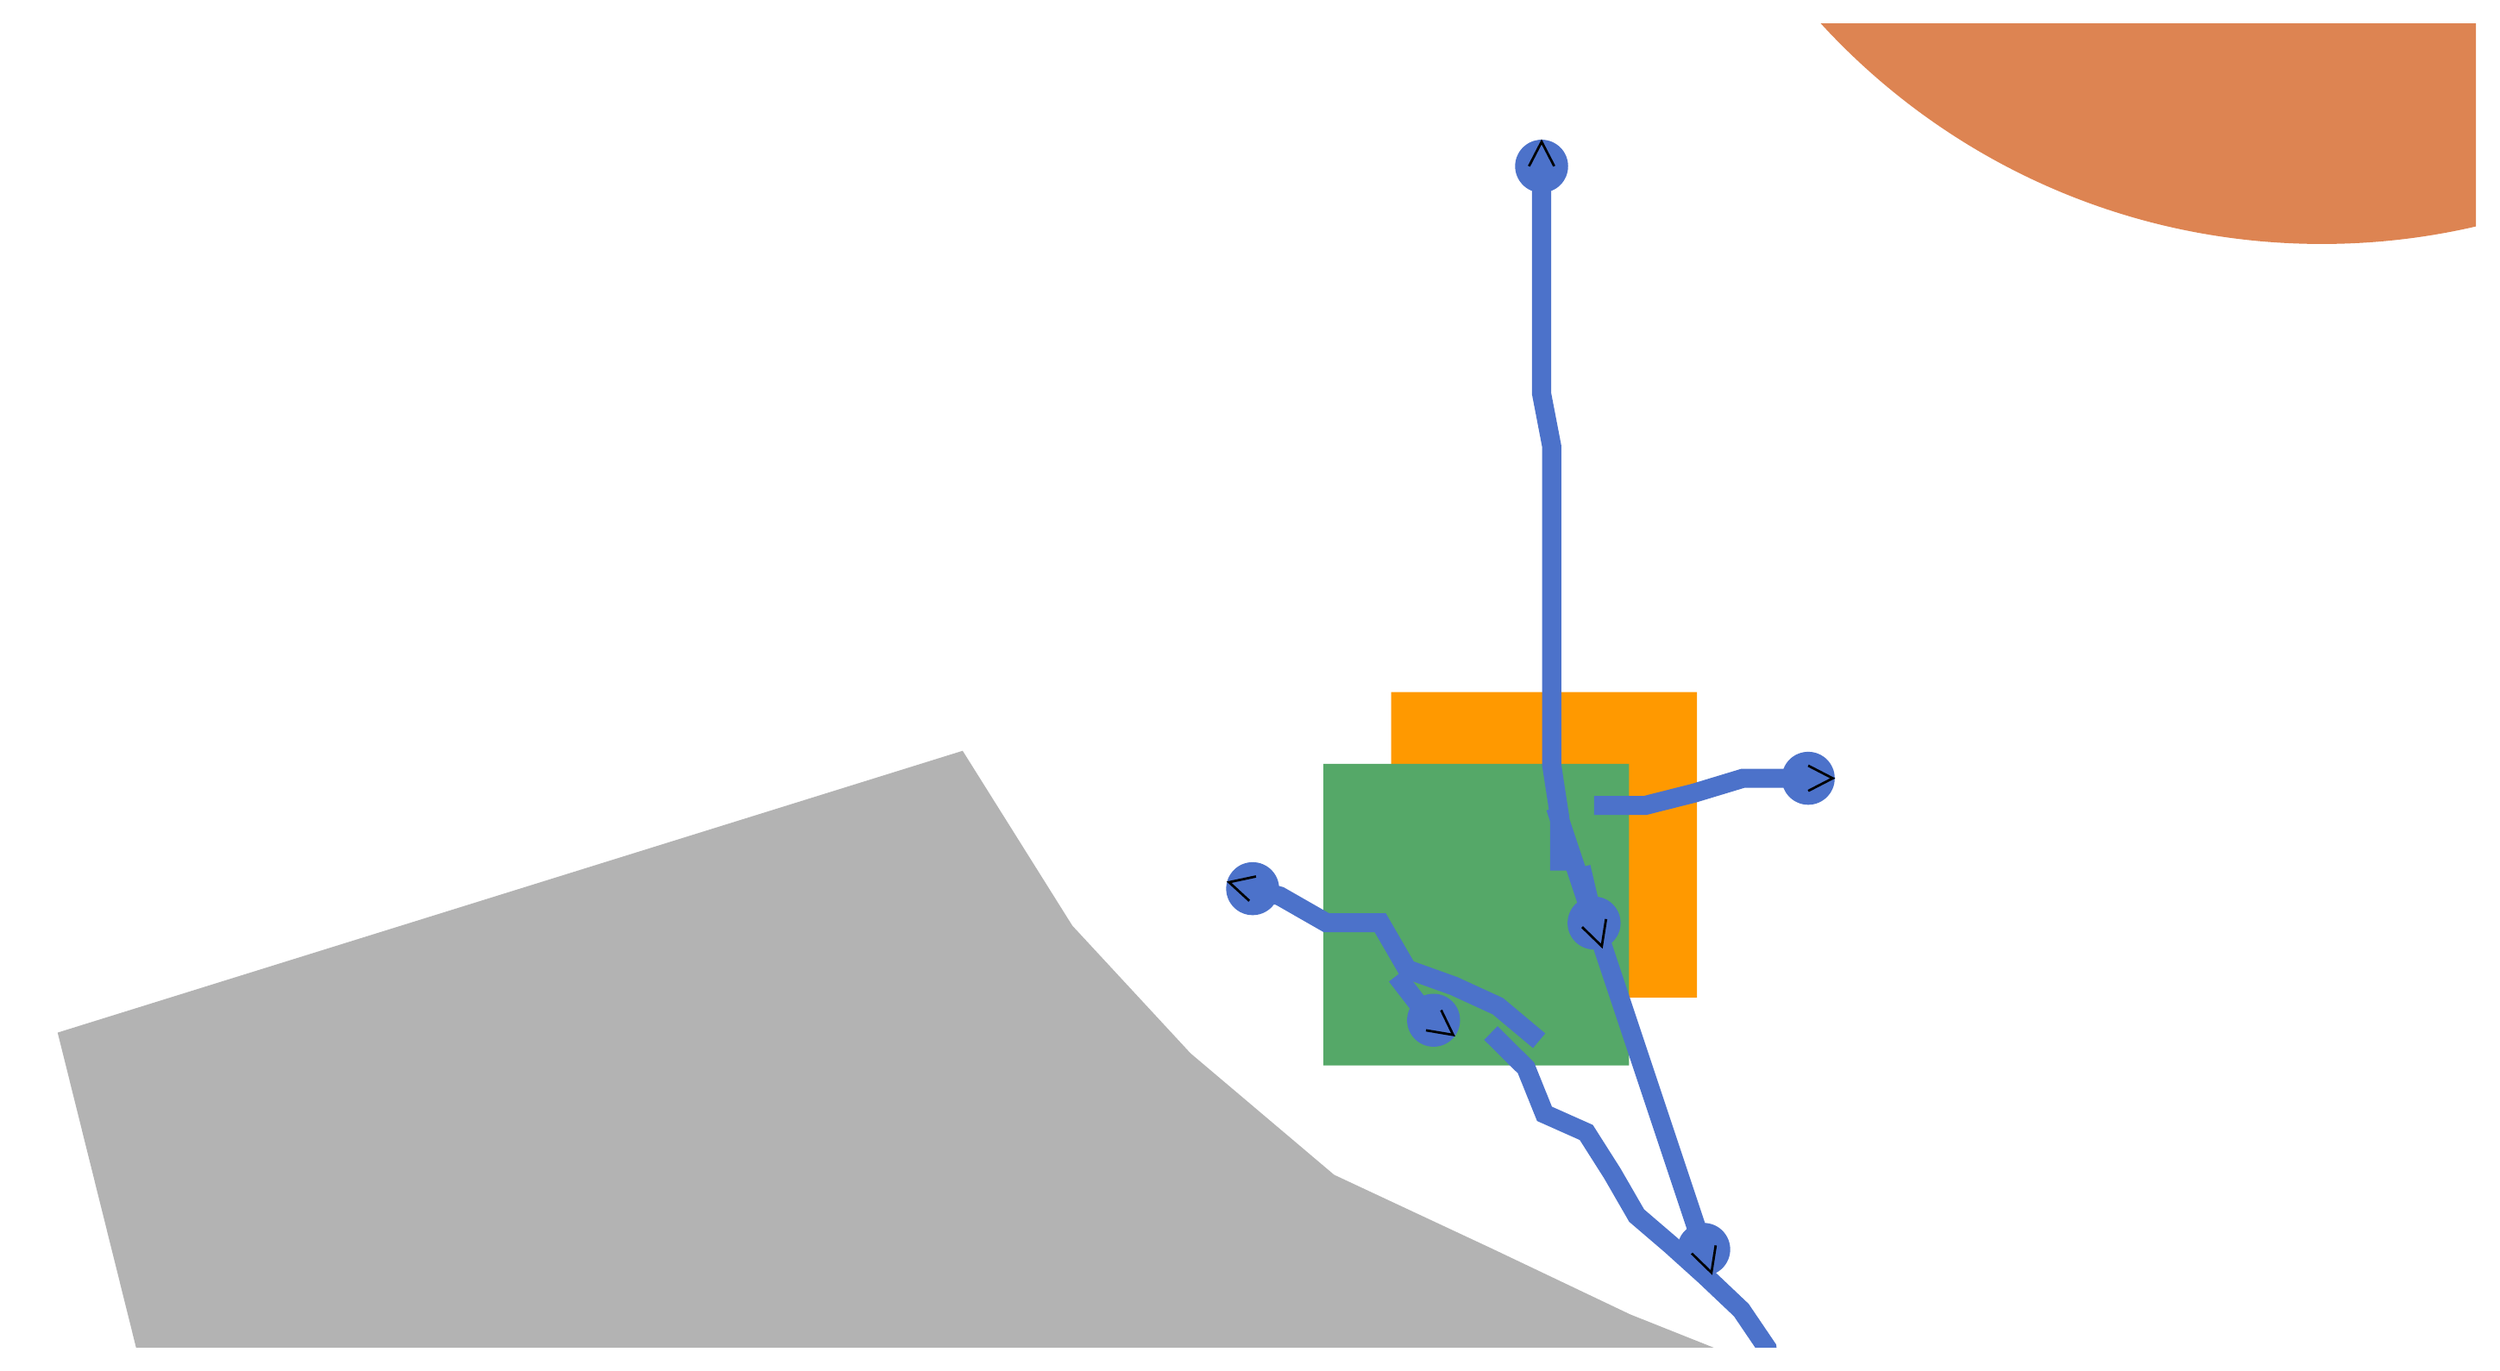
\begin{tikzpicture}
[x=1cm,y=1cm,
trajectory/.style={line width=8, opacity=1.0},
pedestrian/.style={circle, fill=AgentColor, minimum size=0.780000 cm},
walkdirection/.style={black, line width=1},
selected/.style={draw=magenta, line width=2},
group/.style={},
voronoi/.style={black, line width=1}
]

% Clipping
\clip (163.872000,152.856000) rectangle (199.968000,172.344000);
% Ground
\fill[white] (0.000000,0.000000) rectangle (402.000000,369.000000);
% Target Changers
\coordinate (TargetChanger97) at (186.250000,160.250000); % Centroid: TargetChanger 97
\fill[TargetChangerColor] (184.000000,158.000000) to (188.500000,158.000000) to (188.500000,162.500000) to (184.000000,162.500000) to (184.000000,158.000000);
\coordinate (TargetChanger97) at (216.750000,169.250000); % Centroid: TargetChanger 97
\fill[TargetChangerColor] (214.500000,167.000000) to (219.000000,167.000000) to (219.000000,171.500000) to (214.500000,171.500000) to (214.500000,167.000000);
\coordinate (TargetChanger97) at (210.750000,198.750000); % Centroid: TargetChanger 97
\fill[TargetChangerColor] (208.500000,196.500000) to (213.000000,196.500000) to (213.000000,201.000000) to (208.500000,201.000000) to (208.500000,196.500000);
\coordinate (TargetChanger97) at (180.250000,191.750000); % Centroid: TargetChanger 97
\fill[TargetChangerColor] (178.000000,189.500000) to (182.500000,189.500000) to (182.500000,194.000000) to (178.000000,194.000000) to (178.000000,189.500000);
% Sources
\coordinate (Source1) at (201.000000,7.500000); % Centroid: Source 1
\fill[SourceColor] (5.000000,5.000000) to (397.000000,5.000000) to (397.000000,10.000000) to (5.000000,10.000000) to (5.000000,5.000000);
\coordinate (Source3) at (201.000000,361.500000); % Centroid: Source 3
\fill[SourceColor] (5.000000,359.000000) to (397.000000,359.000000) to (397.000000,364.000000) to (5.000000,364.000000) to (5.000000,359.000000);
\coordinate (Source2) at (394.500000,184.500000); % Centroid: Source 2
\fill[SourceColor] (392.000000,10.000000) to (397.000000,10.000000) to (397.000000,359.000000) to (392.000000,359.000000) to (392.000000,10.000000);
\coordinate (Source4) at (7.500000,184.500000); % Centroid: Source 4
\fill[SourceColor] (5.000000,10.000000) to (10.000000,10.000000) to (10.000000,359.000000) to (5.000000,359.000000) to (5.000000,10.000000);
\coordinate (Source8) at (179.250000,190.750000); % Centroid: Source 8
\fill[SourceColor] (177.000000,188.500000) to (181.500000,188.500000) to (181.500000,193.000000) to (177.000000,193.000000) to (177.000000,188.500000);
\coordinate (Source7) at (209.750000,197.750000); % Centroid: Source 7
\fill[SourceColor] (207.500000,195.500000) to (212.000000,195.500000) to (212.000000,200.000000) to (207.500000,200.000000) to (207.500000,195.500000);
\coordinate (Source6) at (215.750000,168.250000); % Centroid: Source 6
\fill[SourceColor] (213.500000,166.000000) to (218.000000,166.000000) to (218.000000,170.500000) to (213.500000,170.500000) to (213.500000,166.000000);
\coordinate (Source5) at (185.250000,159.221920); % Centroid: Source 5
\fill[SourceColor] (183.000000,157.000000) to (187.500000,157.000000) to (187.500000,161.443848) to (183.000000,161.443848) to (183.000000,157.000000);
% Targets
\coordinate (Target1) at (201.000000,2.500000); % Centroid: Target 1
\fill[TargetColor] (0.000000,0.000000) to (402.000000,0.000000) to (402.000000,5.000000) to (0.000000,5.000000) to (0.000000,0.000000);
\coordinate (Target3) at (201.000000,366.500000); % Centroid: Target 3
\fill[TargetColor] (0.000000,364.000000) to (402.000000,364.000000) to (402.000000,369.000000) to (0.000000,369.000000) to (0.000000,364.000000);
\coordinate (Target2) at (399.500000,184.500000); % Centroid: Target 2
\fill[TargetColor] (397.000000,5.000000) to (402.000000,5.000000) to (402.000000,364.000000) to (397.000000,364.000000) to (397.000000,5.000000);
\coordinate (Target4) at (2.500000,184.500000); % Centroid: Target 4
\fill[TargetColor] (0.000000,5.000000) to (5.000000,5.000000) to (5.000000,364.000000) to (0.000000,364.000000) to (0.000000,5.000000);
\coordinate (Target0) at (197.700000,179.100000); % Centroid: Target 0
\fill[TargetColor] (207.699997,179.100006) .. controls (207.699997,184.622849) and (203.222855,189.100006) .. (197.699997,189.100006) .. controls (192.177155,189.100006) and (187.699997,184.622849) .. (187.699997,179.100006) .. controls (187.699997,173.577148) and (192.177155,169.100006) .. (197.699997,169.100006) .. controls (203.222855,169.100006) and (207.699997,173.577148) .. (207.699997,179.100006);
% Absorbing Areas
% Obstacles
\coordinate (Obstacle1) at (295.081319,330.436524); % Centroid: Obstacle 1
\fill[ObstacleColor] (290.433899,318.961853) to (284.447906,339.328033) to (299.101868,344.076691) to (303.460022,330.873688) to (306.038727,323.380280) to (298.465729,320.723480) to (297.930664,317.172699) to (293.437866,315.872375) to (290.433899,318.961853);
\coordinate (Obstacle2) at (329.118007,344.805938); % Centroid: Obstacle 2
\fill[ObstacleColor] (320.778595,339.790955) to (317.479462,349.895233) to (334.461426,355.514526) to (339.190521,337.270630) to (330.338135,334.463562) to (326.087799,336.379639) to (324.689972,341.035187) to (320.778595,339.790955);
\coordinate (Obstacle3) at (339.825437,282.106834); % Centroid: Obstacle 3
\fill[ObstacleColor] (331.814148,262.787994) to (322.255615,293.492706) to (335.098358,297.480255) to (347.831421,301.430145) to (357.397491,270.714661) to (345.137787,266.916870) to (331.814148,262.787994);
\coordinate (Obstacle4) at (300.713239,309.409639); % Centroid: Obstacle 4
\fill[ObstacleColor] (296.528442,301.684418) to (293.250122,311.967682) to (297.161530,313.211884) to (296.552185,315.114441) to (301.891205,316.804199) to (304.322052,317.533966) to (308.159882,305.379578) to (306.142609,304.732788) to (296.528442,301.684418);
\coordinate (Obstacle5) at (311.230072,313.042894); % Centroid: Obstacle 5
\fill[ObstacleColor] (308.159882,305.379578) to (304.322052,317.533966) to (306.065308,318.080933) to (314.237518,320.694336) to (318.195435,308.667145) to (310.198395,306.016052) to (308.159882,305.379578);
\coordinate (Obstacle6) at (321.472361,317.810288); % Centroid: Obstacle 6
\fill[ObstacleColor] (318.195435,308.667145) to (314.237518,320.694336) to (313.465546,323.024841) to (324.755249,327.107544) to (326.666168,320.879700) to (329.484772,312.404663) to (318.195435,308.667145);
\coordinate (Obstacle7) at (332.020257,332.192724); % Centroid: Obstacle 7
\fill[ObstacleColor] (335.571991,330.492523) to (340.828613,332.156799) to (339.190521,337.270630) to (330.338135,334.463562) to (323.194763,332.191010) to (324.057373,329.496582) to (324.755249,327.107544) to (329.496399,328.629181) to (335.571991,330.492523);
\coordinate (Obstacle8) at (265.914898,326.233073); % Centroid: Obstacle 8
\fill[ObstacleColor] (261.546509,316.473999) to (257.967285,327.703156) to (259.214294,331.170410) to (271.844543,335.260864) to (274.616669,326.728302) to (270.754700,325.463776) to (270.647369,319.502228) to (261.546509,316.473999);
\coordinate (Obstacle9) at (278.437916,331.219980); % Centroid: Obstacle 9
\fill[ObstacleColor] (274.616669,326.728302) to (271.844543,335.260864) to (281.614319,338.415497) to (284.883148,327.129669) to (275.364838,323.940338) to (274.616669,326.728302);
\coordinate (Obstacle10) at (272.024300,301.107052); % Centroid: Obstacle 10
\fill[ObstacleColor] (269.153290,293.743683) to (265.283966,305.284424) to (274.885590,308.477020) to (278.769226,296.925720) to (269.153290,293.743683);
\coordinate (Obstacle11) at (282.424889,293.093499); % Centroid: Obstacle 11
\fill[ObstacleColor] (278.769226,296.925720) to (269.153290,293.743683) to (272.183441,284.653320) to (295.694824,292.442963) to (292.664612,301.533356) to (283.165314,298.389252) to (278.769226,296.925720);
\coordinate (Obstacle12) at (284.018539,312.755195); % Centroid: Obstacle 12
\fill[ObstacleColor] (283.165314,298.389252) to (292.664612,301.533356) to (284.883148,327.129669) to (275.364838,323.940338) to (283.165314,298.389252);
\coordinate (Obstacle13) at (178.203269,148.228028); % Centroid: Obstacle 13
\fill[ObstacleColor] (188.944641,152.765671) to (191.966888,138.363434) to (176.529526,135.154572) to (174.956818,142.687332) to (168.462982,141.030563) to (164.367126,157.484283) to (177.690277,161.634949) to (179.305511,159.059006) to (181.046432,157.178375) to (183.158905,155.390198) to (185.487244,154.300842) to (187.519028,153.333527) to (188.944641,152.765671);
\coordinate (Obstacle14) at (189.018613,60.280969); % Centroid: Obstacle 14
\fill[ObstacleColor] (199.779663,97.557487) to (166.860718,86.728302) to (169.326950,79.976501) to (173.349609,68.953911) to (175.184891,63.591637) to (164.180206,59.665203) to (162.620758,64.013824) to (150.102905,59.872410) to (152.164566,53.516800) to (161.381317,38.298717) to (165.581696,39.799053) to (170.297134,41.453140) to (172.347900,42.134571) to (175.713531,33.703087) to (178.174606,26.728384) to (196.897324,32.459682) to (220.759048,39.850609) to (221.792755,44.155800) to (218.301285,53.139099) to (215.851013,59.835827) to (208.597733,80.987679) to (205.339432,91.472214) to (204.110321,95.900543) to (199.779663,97.557487);
\coordinate (Obstacle15) at (131.250614,56.723092); % Centroid: Obstacle 15
\fill[ObstacleColor] (138.706100,76.653351) to (144.090942,78.600815) to (148.402817,66.576202) to (150.102905,59.872410) to (145.406967,58.252510) to (143.062683,57.437138) to (147.986084,42.919857) to (122.377518,34.002331) to (110.077515,66.259407) to (128.423309,72.922234) to (134.917633,75.280479) to (138.706100,76.653351);
\coordinate (Obstacle16) at (70.477268,212.814010); % Centroid: Obstacle 16
\fill[ObstacleColor] (10.837765,246.660507) to (10.000000,249.433868) to (27.987135,255.302887) to (37.364380,258.374908) to (55.522709,264.306396) to (70.497459,269.211670) to (84.969696,273.997131) to (92.919334,261.145813) to (105.189072,240.323410) to (111.743927,229.210403) to (123.835159,208.692841) to (129.579666,198.940109) to (138.538147,183.745316) to (135.015839,178.229401) to (120.123589,174.585449) to (102.094093,170.150894) to (45.719292,156.324066) to (38.144627,161.707245) to (17.865507,224.675613) to (15.535628,232.212265) to (10.837765,246.660507);
\coordinate (Obstacle17) at (154.647870,210.024301); % Centroid: Obstacle 17
\fill[ObstacleColor] (149.467056,200.630142) to (143.004929,210.789108) to (152.715942,215.277405) to (161.723297,219.459839) to (165.162231,208.971207) to (149.467056,200.630142);
\coordinate (Obstacle18) at (245.865667,131.115455); % Centroid: Obstacle 18
\fill[ObstacleColor] (273.575867,118.592270) to (259.176788,143.918808) to (252.541626,156.364746) to (241.362488,152.108383) to (242.261292,147.244019) to (238.240448,146.485550) to (231.215073,144.741119) to (230.701126,146.691956) to (218.495621,143.453384) to (221.018539,133.474609) to (223.548416,123.496101) to (226.078293,113.517593) to (237.031723,116.796326) to (242.912048,118.863480) to (242.114960,120.948013) to (255.637680,124.260399) to (257.907928,123.413780) to (259.264374,120.883430) to (251.617386,117.444382) to (258.866486,105.646011) to (272.015930,113.531570) to (272.909393,114.847046) to (273.618927,117.135239) to (273.575867,118.592270);
\coordinate (Obstacle19) at (274.290763,62.472991); % Centroid: Obstacle 19
\fill[ObstacleColor] (270.637756,20.643244) to (266.277588,21.809029) to (259.722290,31.496548) to (258.665161,32.234692) to (254.015076,41.529011) to (246.448715,56.288094) to (241.697220,65.333481) to (241.675491,65.889389) to (242.037460,66.582787) to (236.245651,77.892509) to (237.842087,82.553757) to (255.808350,93.411339) to (262.725616,97.211601) to (276.689789,104.872902) to (281.507782,103.546867) to (285.028961,97.537872) to (290.030640,88.847496) to (307.955933,58.458740) to (315.757324,45.156509) to (308.905396,41.993439) to (299.317413,36.307060) to (270.637756,20.643244);
\coordinate (Obstacle20) at (329.864960,105.111829); % Centroid: Obstacle 20
\fill[ObstacleColor] (298.607697,100.485100) to (304.282898,90.384621) to (323.476929,100.755966) to (326.853821,94.529785) to (330.144379,88.734505) to (333.402924,82.514839) to (335.582947,78.290749) to (339.765656,70.114021) to (343.592773,62.680576) to (350.431152,66.188362) to (357.272583,69.618324) to (349.620056,84.797043) to (353.892670,86.935074) to (355.794220,87.877991) to (362.055115,90.873253) to (356.135040,103.146606) to (354.197388,107.213135) to (352.266663,111.279945) to (349.839813,116.485413) to (343.221924,130.969666) to (341.249298,130.068512) to (338.164612,128.645065) to (335.729370,127.491982) to (333.881592,126.595718) to (332.929688,128.551697) to (331.397125,131.676453) to (329.925262,134.669952) to (327.642883,139.201828) to (327.095612,140.227142) to (307.454315,129.749207) to (310.324677,124.394035) to (303.675812,120.838036) to (291.160645,113.968231) to (298.607697,100.485100);
\coordinate (Obstacle21) at (293.364322,128.684080); % Centroid: Obstacle 21
\fill[ObstacleColor] (303.087280,135.179489) to (305.870789,130.978973) to (287.438660,120.314560) to (282.903137,128.811584) to (294.917084,135.528152) to (297.454285,131.763428) to (303.087280,135.179489);
\coordinate (Obstacle22) at (315.487822,91.697358); % Centroid: Obstacle 22
\fill[ObstacleColor] (311.460022,84.340424) to (308.445984,82.708183) to (304.282898,90.384621) to (323.476929,100.755966) to (326.853821,94.529785) to (326.262024,94.205994) to (321.553680,91.661217) to (322.339905,90.210968) to (311.460022,84.340424);
\coordinate (Obstacle23) at (341.827541,153.229148); % Centroid: Obstacle 23
\fill[ObstacleColor] (335.944946,138.502029) to (334.028229,137.591934) to (332.924133,139.709000) to (325.568817,154.220123) to (327.601257,155.368576) to (329.356232,156.328018) to (341.671295,160.139053) to (345.078156,161.140823) to (342.565308,171.921692) to (348.832306,173.514145) to (350.731262,166.528671) to (351.713684,162.903595) to (352.029907,161.746765) to (353.585999,153.756836) to (354.290100,150.143143) to (355.014435,147.610367) to (353.159302,146.724945) to (350.591827,145.577820) to (348.010101,144.263107) to (339.498291,140.199921) to (335.944946,138.502029);
\coordinate (Obstacle24) at (252.937310,170.203926); % Centroid: Obstacle 24
\fill[ObstacleColor] (252.592590,167.680130) to (250.740479,171.516205) to (253.277588,172.728897) to (255.136642,168.893097) to (252.592590,167.680130);
\coordinate (Obstacle25) at (268.999679,312.875246); % Centroid: Obstacle 25
\fill[ObstacleColor] (270.647369,319.502228) to (261.546509,316.473999) to (265.283966,305.284424) to (274.885590,308.477020) to (276.538666,309.020447) to (275.397644,312.438904) to (274.108307,312.009888) to (272.849731,315.768951) to (275.119751,316.525818) to (273.774475,320.548706) to (270.647369,319.502228);
\coordinate (Obstacle26) at (303.677226,260.542214); % Centroid: Obstacle 26
\fill[ObstacleColor] (297.961212,261.308380) to (308.723480,264.847046) to (306.517273,271.519867) to (304.980804,271.014404) to (302.373444,278.885284) to (311.400208,281.855011) to (319.831726,256.339813) to (285.699677,245.295303) to (284.513824,245.772293) to (281.857910,253.641296) to (291.280548,256.793518) to (298.646912,259.230621) to (297.961212,261.308380);
\coordinate (Obstacle27) at (331.393194,234.311307); % Centroid: Obstacle 27
\fill[ObstacleColor] (322.429474,245.695877) to (330.345184,220.227325) to (330.442322,219.874802) to (334.632599,220.740189) to (336.706726,221.177628) to (338.133118,221.478378) to (339.282745,222.815033) to (339.658936,224.210510) to (333.155548,247.317932) to (331.397766,248.563156) to (326.389038,246.953110) to (322.429474,245.695877);
\coordinate (Obstacle28) at (285.452926,265.267328); % Centroid: Obstacle 28
\fill[ObstacleColor] (292.375092,275.710541) to (278.366058,270.808929) to (277.378906,270.291534) to (276.752472,269.610077) to (276.544891,268.699982) to (276.761353,267.606079) to (281.857910,253.641296) to (291.280548,256.793518) to (288.409119,265.199707) to (295.176270,267.502014) to (292.375092,275.710541);
\coordinate (Obstacle29) at (298.687608,273.270388); % Centroid: Obstacle 29
\fill[ObstacleColor] (302.373444,278.885284) to (304.980804,271.014404) to (295.176270,267.502014) to (292.375092,275.710541) to (302.373444,278.885284);
\coordinate (Obstacle30) at (236.254037,230.284147); % Centroid: Obstacle 30
\fill[ObstacleColor] (224.872101,197.530304) to (218.625458,195.949936) to (212.656540,201.662872) to (205.421356,205.466736) to (196.778854,245.460785) to (206.909134,248.462326) to (206.252930,251.031189) to (215.453644,253.996414) to (216.448380,252.365005) to (240.916794,260.381104) to (240.469177,262.412506) to (250.959656,265.795654) to (251.781876,263.778931) to (257.488190,265.494110) to (260.338531,264.202484) to (276.457977,214.055969) to (275.547363,211.225433) to (224.849380,199.533752) to (224.872101,197.530304);
\coordinate (Obstacle31) at (120.027878,263.408046); % Centroid: Obstacle 31
\fill[ObstacleColor] (111.429146,261.634979) to (125.262947,269.780762) to (128.305145,264.643768) to (126.665054,263.766846) to (124.357750,262.540894) to (114.522011,257.156952) to (112.354851,260.702393) to (111.429146,261.634979);
\coordinate (Obstacle32) at (153.319207,271.059361); % Centroid: Obstacle 32
\fill[ObstacleColor] (165.214127,249.961990) to (153.275955,246.110443) to (151.151413,253.187378) to (153.719315,253.966965) to (153.068390,256.046082) to (150.934799,262.643860) to (149.292953,267.857788) to (148.529388,268.908081) to (147.805756,269.113647) to (146.588318,269.333344) to (144.857590,268.998474) to (140.374283,267.631836) to (138.423355,272.399445) to (142.982529,273.780182) to (146.800339,274.931488) to (149.828659,275.840424) to (149.468292,276.884186) to (148.898468,278.665833) to (146.105988,277.944275) to (144.624649,282.251404) to (142.838882,287.415192) to (140.921280,293.108337) to (150.827301,296.691162) to (151.469849,296.248596) to (152.219925,295.899292) to (153.925903,290.999634) to (154.222549,289.808624) to (155.031754,287.412781) to (155.495331,285.860809) to (157.644974,279.386169) to (158.747757,276.055267) to (160.905212,269.558655) to (161.984589,266.293671) to (164.135101,259.796783) to (166.741821,251.936951) to (165.214127,249.961990);
\coordinate (Obstacle33) at (133.708370,271.977672); % Centroid: Obstacle 33
\fill[ObstacleColor] (131.446564,266.392242) to (122.301025,286.378998) to (132.076996,289.912170) to (138.423355,272.399445) to (140.374283,267.631836) to (141.103653,265.856445) to (145.491135,267.364075) to (147.485092,261.139435) to (136.104034,257.610352) to (135.041641,260.085388) to (130.167770,257.690216) to (126.665054,263.766846) to (131.446564,266.392242);
\coordinate (Obstacle34) at (141.766697,283.572558); % Centroid: Obstacle 34
\fill[ObstacleColor] (142.982529,273.780182) to (136.495667,291.510132) to (138.085037,292.084442) to (140.921280,293.108337) to (142.838882,287.415192) to (144.624649,282.251404) to (146.800339,274.931488) to (142.982529,273.780182);
\coordinate (Obstacle35) at (127.713523,249.210113); % Centroid: Obstacle 35
\fill[ObstacleColor] (137.241531,253.924484) to (140.746841,242.091064) to (138.695724,241.420761) to (136.733475,240.787354) to (127.580391,237.846390) to (126.648209,238.233124) to (124.772125,239.306763) to (116.333618,254.176682) to (115.093071,256.232788) to (114.522011,257.156952) to (124.357750,262.540894) to (126.178894,259.672363) to (130.139969,252.355362) to (133.265442,252.911743) to (137.241531,253.924484);
\coordinate (Obstacle36) at (202.032497,301.341363); % Centroid: Obstacle 36
\fill[ObstacleColor] (207.894638,293.108582) to (202.000168,311.496307) to (196.104874,309.640167) to (202.196167,291.015137) to (207.894638,293.108582);
\coordinate (Obstacle37) at (248.801396,286.469121); % Centroid: Obstacle 37
\fill[ObstacleColor] (248.053894,284.678802) to (250.655563,276.596100) to (255.856369,278.091095) to (256.228180,279.954071) to (252.499313,291.990265) to (251.552994,295.048859) to (242.845749,292.258728) to (240.320801,291.447388) to (241.620987,287.333618) to (240.624695,287.049713) to (242.111755,282.776245) to (248.053894,284.678802);
\coordinate (Obstacle38) at (238.795823,317.063769); % Centroid: Obstacle 38
\fill[ObstacleColor] (237.111191,310.107086) to (245.804535,312.896637) to (242.928299,322.494141) to (241.441956,323.905884) to (231.549438,320.869019) to (234.058304,312.671326) to (234.368362,311.848297) to (236.374344,312.605957) to (237.111191,310.107086);
\coordinate (Obstacle39) at (166.377121,207.600407); % Centroid: Obstacle 39
\fill[ObstacleColor] (159.621933,183.800705) to (149.467056,200.630142) to (165.162231,208.971207) to (161.723297,219.459839) to (160.256653,223.923447) to (156.762756,233.151657) to (167.264130,236.969345) to (171.750000,233.648163) to (173.207764,226.389282) to (179.387405,198.035492) to (175.444977,193.137833) to (173.576828,186.539597) to (159.621933,183.800705);
\coordinate (Obstacle40) at (193.189868,287.996192); % Centroid: Obstacle 40
\fill[ObstacleColor] (195.544586,275.444275) to (201.710892,277.299835) to (206.044144,278.950195) to (202.196167,291.015137) to (196.104874,309.640167) to (182.690231,305.174072) to (180.612122,300.928284) to (193.079651,261.896576) to (195.962112,259.960327) to (199.997604,260.697083) to (195.544586,275.444275);
\coordinate (Obstacle41) at (216.000222,273.770896); % Centroid: Obstacle 41
\fill[ObstacleColor] (210.946671,280.433472) to (215.778244,265.422699) to (221.054916,267.109924) to (218.058212,276.413208) to (217.093719,279.404297) to (216.223328,282.120697) to (210.946671,280.433472);
\coordinate (Obstacle42) at (233.920833,277.732647); % Centroid: Obstacle 42
\fill[ObstacleColor] (226.994980,282.575104) to (230.949265,270.280457) to (241.090729,273.527496) to (238.489075,281.610199) to (237.974731,283.215820) to (235.593704,282.454651) to (234.755402,285.060944) to (228.223221,282.968292) to (226.994980,282.575104);
\coordinate (Obstacle43) at (235.208888,299.935434); % Centroid: Obstacle 43
\fill[ObstacleColor] (240.320801,291.447388) to (251.552994,295.048859) to (245.804535,312.896637) to (237.111191,310.107086) to (237.253860,309.656097) to (218.439911,303.620361) to (223.586349,287.664307) to (239.855026,292.876770) to (240.320801,291.447388);
\coordinate (Obstacle44) at (175.883021,336.586164); % Centroid: Obstacle 44
\fill[ObstacleColor] (171.533463,322.933075) to (163.404434,349.440186) to (176.654221,353.855255) to (181.794083,336.640625) to (186.477173,338.048492) to (190.156845,326.377808) to (188.241898,325.779633) to (175.772400,321.840424) to (174.070313,321.306244) to (171.533463,322.933075);
\coordinate (Obstacle45) at (146.957587,222.746597); % Centroid: Obstacle 45
\fill[ObstacleColor] (152.715942,215.277405) to (143.004929,210.789108) to (133.640274,225.355576) to (156.762756,233.151657) to (160.256653,223.923447) to (149.543976,221.600769) to (152.715942,215.277405);
\coordinate (Obstacle46) at (208.666322,271.437817); % Centroid: Obstacle 46
\fill[ObstacleColor] (201.710892,277.299835) to (206.163925,262.552673) to (215.778244,265.422699) to (210.946671,280.433472) to (206.044144,278.950195) to (201.710892,277.299835);
\coordinate (Obstacle47) at (224.323817,274.652507); % Centroid: Obstacle 47
\fill[ObstacleColor] (218.058212,276.413208) to (221.054916,267.109924) to (230.949265,270.280457) to (226.994980,282.575104) to (219.254929,280.101196) to (220.219437,277.110107) to (218.058212,276.413208);
\coordinate (Obstacle48) at (244.571958,279.103977); % Centroid: Obstacle 48
\fill[ObstacleColor] (238.489075,281.610199) to (241.090729,273.527496) to (250.655563,276.596100) to (248.053894,284.678802) to (242.111755,282.776245) to (238.489075,281.610199);
\coordinate (Obstacle49) at (200.257450,343.706310); % Centroid: Obstacle 49
\fill[ObstacleColor] (193.521774,350.316437) to (200.080582,329.504913) to (200.938126,329.783386) to (208.638214,332.211151) to (201.043823,355.699219) to (200.287521,357.985779) to (197.309982,357.023132) to (196.239578,356.680634) to (191.924149,355.287140) to (193.521774,350.316437);
\coordinate (Obstacle51) at (67.291007,288.651763); % Centroid: Obstacle 51
\fill[ObstacleColor] (61.837215,290.832092) to (54.313457,288.333496) to (56.612133,281.241058) to (80.399513,289.085022) to (78.137238,295.956177) to (61.837215,290.832092);
\coordinate (Obstacle52) at (70.045936,301.650852); % Centroid: Obstacle 52
\fill[ObstacleColor] (49.547863,303.090851) to (54.313457,288.333496) to (61.837215,290.832092) to (90.326782,299.950989) to (86.038864,314.749237) to (77.873482,312.492798) to (49.547863,303.090851);
\coordinate (Obstacle53) at (192.296279,337.996437); % Centroid: Obstacle 53
\fill[ObstacleColor] (186.477173,338.048492) to (190.156845,326.377808) to (194.521729,327.751007) to (199.030548,329.174347) to (200.080582,329.504913) to (193.521774,350.316437) to (185.144073,347.628387) to (188.096436,338.746490) to (186.477173,338.048492);
\coordinate (Obstacle54) at (60.257167,312.976146); % Centroid: Obstacle 54
\fill[ObstacleColor] (77.873482,312.492798) to (49.547863,303.090851) to (45.439243,315.791565) to (63.958054,321.915344) to (65.723366,316.561432) to (75.477219,319.770721) to (77.873482,312.492798);
\coordinate (Obstacle55) at (209.702017,345.267923); % Centroid: Obstacle 55
\fill[ObstacleColor] (208.638214,332.211151) to (218.465683,335.312256) to (213.563446,350.709961) to (212.586243,350.471344) to (210.098236,358.669861) to (201.043823,355.699219) to (208.638214,332.211151);
\coordinate (Obstacle56) at (116.785925,277.158615); % Centroid: Obstacle 56
\fill[ObstacleColor] (119.924362,278.925781) to (105.885948,270.682953) to (102.084984,276.926117) to (102.461159,279.212372) to (122.301025,286.378998) to (131.446564,266.392242) to (128.305145,264.643768) to (125.262947,269.780762) to (119.924362,278.925781);
\coordinate (Obstacle57) at (223.854917,159.016236); % Centroid: Obstacle 57
\fill[ObstacleColor] (229.761169,175.718170) to (232.646072,166.432800) to (230.722610,163.562668) to (231.446838,161.564362) to (227.526230,155.219940) to (230.701126,146.691956) to (218.495621,143.453384) to (216.201294,152.205093) to (214.472824,160.344208) to (217.917648,163.752594) to (220.102142,166.521561) to (222.358124,169.950302) to (223.148148,174.090073) to (229.761169,175.718170);
\coordinate (Obstacle58) at (240.073964,170.133034); % Centroid: Obstacle 58
\fill[ObstacleColor] (232.177795,176.458466) to (229.761169,175.718170) to (232.646072,166.432800) to (237.773712,168.025116) to (240.507278,159.234909) to (249.115494,161.898651) to (243.496994,179.974228) to (232.177795,176.458466);
\coordinate (Obstacle59) at (245.851086,157.225167); % Centroid: Obstacle 59
\fill[ObstacleColor] (240.507278,159.234909) to (249.115494,161.898651) to (252.541626,156.364746) to (241.362488,152.108383) to (240.507278,159.234909);
\coordinate (Obstacle60) at (267.874887,168.404701); % Centroid: Obstacle 60
\fill[ObstacleColor] (268.067535,184.319809) to (270.787903,173.558151) to (269.219757,173.151657) to (272.277069,166.211441) to (274.414429,167.341705) to (279.756073,157.239304) to (270.386322,152.196213) to (268.309723,154.843170) to (257.312195,178.821686) to (257.175171,179.128128) to (257.280853,180.334854) to (258.352081,181.545929) to (264.828918,183.458267) to (268.067535,184.319809);
\coordinate (Obstacle61) at (343.761879,237.870674); % Centroid: Obstacle 61
\fill[ObstacleColor] (342.497589,223.219131) to (339.610107,234.341675) to (335.637817,250.109726) to (345.041412,252.682266) to (345.517670,250.807892) to (349.064514,236.682358) to (351.431976,227.131821) to (351.877014,225.345322) to (347.235413,224.295242) to (342.497589,223.219131);
\coordinate (Obstacle62) at (326.663780,70.442495); % Centroid: Obstacle 62
\fill[ObstacleColor] (324.641327,85.902542) to (310.798553,78.334938) to (317.689392,65.576141) to (320.393677,60.559669) to (324.453186,53.046219) to (343.592773,62.680576) to (339.765656,70.114021) to (337.152649,68.709015) to (334.299164,73.986885) to (330.531525,80.966110) to (333.402924,82.514839) to (330.144379,88.734505) to (324.641327,85.902542);
\coordinate (Obstacle63) at (288.192793,135.555618); % Centroid: Obstacle 63
\fill[ObstacleColor] (282.903137,128.811584) to (279.439178,134.956451) to (291.643005,141.791779) to (293.816010,137.923721) to (297.521088,140.006119) to (298.812469,137.718201) to (294.917084,135.528152) to (282.903137,128.811584);
\coordinate (Obstacle64) at (315.803365,89.464692); % Centroid: Obstacle 64
\fill[ObstacleColor] (324.641327,85.902542) to (310.798553,78.334938) to (308.445984,82.708183) to (304.282898,90.384621) to (323.476929,100.755966) to (326.853821,94.529785) to (326.262024,94.205994) to (321.553680,91.661217) to (322.339905,90.210968) to (324.641327,85.902542);
\coordinate (Obstacle65) at (298.947036,122.564204); % Centroid: Obstacle 65
\fill[ObstacleColor] (303.675812,120.838036) to (291.160645,113.968231) to (287.438660,120.314560) to (305.870789,130.978973) to (307.454315,129.749207) to (310.324677,124.394035) to (303.675812,120.838036);
\coordinate (Obstacle66) at (283.972830,148.528187); % Centroid: Obstacle 66
\fill[ObstacleColor] (291.643005,141.791779) to (279.439178,134.956451) to (270.386322,152.196213) to (279.756073,157.239304) to (288.667572,161.919312) to (296.555237,146.939011) to (297.588196,145.041870) to (291.643005,141.791779);
\coordinate (Obstacle67) at (301.588525,166.026616); % Centroid: Obstacle 67
\fill[ObstacleColor] (313.522156,195.250122) to (316.020721,183.588989) to (321.449738,155.974304) to (319.992126,155.761414) to (321.517853,151.567413) to (325.777679,143.193253) to (327.095612,140.227142) to (307.454315,129.749207) to (305.870789,130.978973) to (303.087280,135.179489) to (297.588196,145.041870) to (296.555237,146.939011) to (288.667572,161.919312) to (283.858917,170.472473) to (274.347565,168.341263) to (273.005981,174.045731) to (270.787903,173.558151) to (268.067535,184.319809) to (313.522156,195.250122);
\coordinate (Obstacle68) at (240.719473,105.439397); % Centroid: Obstacle 68
\fill[ObstacleColor] (237.031723,116.796326) to (226.078293,113.517593) to (230.359787,93.919899) to (235.031754,91.352097) to (258.866486,105.646011) to (251.617386,117.444382) to (239.055359,110.172012) to (237.031723,116.796326);
\coordinate (Obstacle69) at (200.854254,268.998460); % Centroid: Obstacle 69
\fill[ObstacleColor] (195.544586,275.444275) to (199.997604,260.697083) to (206.163925,262.552673) to (201.710892,277.299835) to (195.544586,275.444275);
\coordinate (Obstacle70) at (312.163281,313.381250); % Centroid: Obstacle 70
\fill[ObstacleColor] (318.195435,308.667145) to (310.198395,306.016052) to (306.065308,318.080933) to (314.237518,320.694336) to (318.195435,308.667145);
\coordinate (Obstacle71) at (218.134816,343.599375); % Centroid: Obstacle 71
\fill[ObstacleColor] (213.563446,350.709961) to (218.465683,335.312256) to (222.686615,336.635284) to (217.835983,351.778900) to (213.563446,350.709961);
\coordinate (Obstacle72) at (361.821056,80.794856); % Centroid: Obstacle 72
\fill[ObstacleColor] (363.710083,71.473564) to (369.918121,74.221802) to (369.317932,75.356392) to (365.665497,83.119568) to (362.055115,90.873253) to (355.794220,87.877991) to (353.892670,86.935074) to (360.887512,71.697235) to (363.131134,72.776016) to (363.710083,71.473564);
\coordinate (Obstacle73) at (308.528839,50.128520); % Centroid: Obstacle 73
\fill[ObstacleColor] (315.757324,45.156509) to (307.955933,58.458740) to (301.404083,54.906544) to (308.905396,41.993439) to (315.757324,45.156509);
\coordinate (Obstacle74) at (367.293249,107.672042); % Centroid: Obstacle 74
\fill[ObstacleColor] (387.226685,93.895523) to (379.025818,111.190720) to (376.695038,110.208740) to (375.549713,112.669373) to (369.062347,126.123131) to (371.332397,127.414520) to (364.994659,140.773911) to (364.637299,141.561676) to (362.381592,140.437881) to (359.908203,139.194214) to (360.263397,138.462036) to (350.021759,133.507187) to (349.619751,134.192978) to (346.436676,132.620911) to (343.221924,130.969666) to (349.839813,116.485413) to (352.694702,118.100319) to (355.234283,112.854721) to (352.266663,111.279945) to (354.197388,107.213135) to (357.210083,108.700600) to (359.142548,104.589325) to (356.135040,103.146606) to (362.055115,90.873253) to (365.665497,83.119568) to (369.317932,75.356392) to (391.331055,85.236954) to (387.226685,93.895523);
\coordinate (Obstacle75) at (101.986642,100.248132); % Centroid: Obstacle 75
\fill[ObstacleColor] (100.861824,88.748901) to (103.240364,82.283165) to (112.088074,85.401421) to (109.974892,91.476654) to (107.782349,97.804893) to (100.782799,118.343208) to (91.980240,115.137650) to (100.861824,88.748901);
\coordinate (Obstacle76) at (119.562990,97.409419); % Centroid: Obstacle 76
\fill[ObstacleColor] (120.100723,88.375725) to (124.991295,90.170235) to (119.026878,106.439636) to (114.135887,104.656250) to (116.344894,98.618172) to (120.100723,88.375725);
\coordinate (Obstacle77) at (110.361943,103.199676); % Centroid: Obstacle 77
\fill[ObstacleColor] (109.974892,91.476654) to (107.782349,97.804893) to (100.782799,118.343208) to (108.709137,121.035744) to (114.135887,104.656250) to (116.344894,98.618172) to (120.100723,88.375725) to (112.088074,85.401421) to (109.974892,91.476654);
\coordinate (Obstacle78) at (165.550157,73.195678); % Centroid: Obstacle 78
\fill[ObstacleColor] (160.297623,70.481705) to (162.620758,64.013824) to (164.180206,59.665203) to (175.184891,63.591637) to (173.349609,68.953911) to (169.326950,79.976501) to (166.860718,86.728302) to (155.876450,82.813820) to (160.297623,70.481705);
\coordinate (Obstacle79) at (71.552357,91.488228); % Centroid: Obstacle 79
\fill[ObstacleColor] (77.555244,80.133072) to (86.875549,83.425636) to (81.324486,99.076508) to (73.635262,96.359871) to (69.606316,107.727470) to (57.503880,103.446617) to (64.272087,84.380203) to (67.147545,76.397194) to (77.555244,80.133072);
\coordinate (Obstacle80) at (144.011440,27.652169); % Centroid: Obstacle 80
\fill[ObstacleColor] (122.377518,34.002331) to (147.986084,42.919857) to (153.840073,44.952465) to (156.726990,36.680435) to (160.284393,37.921806) to (161.989136,33.055508) to (163.448944,33.569088) to (164.781143,30.236029) to (167.359299,22.931839) to (130.777054,10.000000) to (122.377518,34.002331);
\coordinate (Obstacle81) at (152.643520,73.508760); % Centroid: Obstacle 81
\fill[ObstacleColor] (155.876450,82.813820) to (160.297623,70.481705) to (156.850800,69.255783) to (158.628387,64.303253) to (154.359528,62.777973) to (152.479599,68.038300) to (150.300522,67.262779) to (148.402817,66.576202) to (144.090942,78.600815) to (145.913635,79.251053) to (155.876450,82.813820);
\coordinate (Obstacle82) at (165.081093,110.451457); % Centroid: Obstacle 82
\fill[ObstacleColor] (169.833496,106.843307) to (166.009125,116.348122) to (160.441376,114.282135) to (163.997803,104.521881) to (169.833496,106.843307);
\coordinate (Obstacle83) at (154.144950,107.453338); % Centroid: Obstacle 83
\fill[ObstacleColor] (158.942078,102.687469) to (154.748611,114.171074) to (149.337372,112.189163) to (153.557266,100.739998) to (158.942078,102.687469);
\coordinate (Obstacle84) at (158.473102,111.833535); % Centroid: Obstacle 84
\fill[ObstacleColor] (163.997803,104.521881) to (160.441376,114.282135) to (158.033264,120.969398) to (152.962799,119.156693) to (154.748611,114.171074) to (158.942078,102.687469) to (163.997803,104.521881);
\coordinate (Obstacle85) at (141.280692,107.243973); % Centroid: Obstacle 85
\fill[ObstacleColor] (147.872009,98.658295) to (140.710648,117.998779) to (134.626953,115.801315) to (136.906647,109.910759) to (141.865036,96.452690) to (147.872009,98.658295);
\coordinate (Obstacle86) at (169.447020,115.834589); % Centroid: Obstacle 86
\fill[ObstacleColor] (175.340118,108.873512) to (169.142303,124.888763) to (163.517365,122.508759) to (166.009125,116.348122) to (169.833496,106.843307) to (175.340118,108.873512);
\coordinate (Obstacle87) at (147.138192,109.297732); % Centroid: Obstacle 87
\fill[ObstacleColor] (153.557266,100.739998) to (149.337372,112.189163) to (146.170883,119.971458) to (140.710648,117.998779) to (147.872009,98.658295) to (153.557266,100.739998);
\coordinate (Obstacle88) at (125.051110,99.433730); % Centroid: Obstacle 88
\fill[ObstacleColor] (131.042496,92.488899) to (126.559837,104.796364) to (125.202072,108.607246) to (119.026878,106.439636) to (124.991295,90.170235) to (131.042496,92.488899);
\coordinate (Obstacle89) at (120.721523,121.293681); % Centroid: Obstacle 89
\fill[ObstacleColor] (131.368790,107.968460) to (136.303757,94.398125) to (131.042496,92.488899) to (126.559837,104.796364) to (126.107109,106.070366) to (125.202072,108.607246) to (119.026878,106.439636) to (114.340530,104.753326) to (108.709137,121.035744) to (104.402245,131.869110) to (112.546188,134.859665) to (108.863686,144.826599) to (113.613319,146.314941) to (116.893456,136.688629) to (126.019409,139.795502) to (128.674606,133.006531) to (134.626953,115.801315) to (131.462418,114.642113) to (132.394333,112.128555) to (127.387154,110.296074) to (128.607880,106.969795) to (131.368790,107.968460);
\coordinate (Obstacle90) at (187.631823,124.408358); % Centroid: Obstacle 90
\fill[ObstacleColor] (176.529526,135.154572) to (191.966888,138.363434) to (198.452560,118.183739) to (197.195129,113.736191) to (184.491364,110.444824) to (182.237106,111.949081) to (176.529526,135.154572);
\coordinate (Obstacle91) at (92.607577,127.977428); % Centroid: Obstacle 91
\fill[ObstacleColor] (91.980240,115.137650) to (84.337646,138.089478) to (93.454132,140.371933) to (100.782799,118.343208) to (91.980240,115.137650);
\coordinate (Obstacle92) at (119.815760,143.051907); % Centroid: Obstacle 92
\fill[ObstacleColor] (122.739693,149.410706) to (126.019409,139.795502) to (116.893456,136.688629) to (113.613319,146.314941) to (122.739693,149.410706);
\coordinate (Obstacle93) at (100.902016,130.291467); % Centroid: Obstacle 93
\fill[ObstacleColor] (100.782799,118.343208) to (93.454132,140.371933) to (100.444832,142.471146) to (104.402245,131.869110) to (108.709137,121.035744) to (100.782799,118.343208);
\coordinate (Obstacle94) at (106.519529,138.496233); % Centroid: Obstacle 94
\fill[ObstacleColor] (104.402245,131.869110) to (100.444832,142.471146) to (108.863686,144.826599) to (112.546188,134.859665) to (104.402245,131.869110);
\coordinate (Obstacle95) at (155.954863,148.193919); % Centroid: Obstacle 95
\fill[ObstacleColor] (148.381744,148.742157) to (147.224991,154.698853) to (160.180557,158.122437) to (166.110489,140.426422) to (162.280853,139.397110) to (160.450989,142.309860) to (156.523819,141.109711) to (149.636307,139.214874) to (147.634338,147.777603) to (148.381744,148.742157);
\coordinate (Obstacle96) at (144.179961,134.903108); % Centroid: Obstacle 96
\fill[ObstacleColor] (134.626953,115.801315) to (128.674606,133.006531) to (126.019409,139.795502) to (122.739693,149.410706) to (146.971710,155.668854) to (147.224991,154.698853) to (148.381744,148.742157) to (147.634338,147.777603) to (149.636307,139.214874) to (160.450989,142.309860) to (162.280853,139.397110) to (169.142303,124.888763) to (158.033264,120.969398) to (152.962799,119.156693) to (151.468750,118.808807) to (150.459641,121.519775) to (146.170883,119.971458) to (140.710648,117.998779) to (134.626953,115.801315);
\coordinate (Obstacle98) at (118.361707,322.327489); % Centroid: Obstacle 98
\fill[ObstacleColor] (121.832779,341.580261) to (122.587143,341.832428) to (135.784088,346.178528) to (136.364349,343.951874) to (137.441956,340.731354) to (138.435883,337.696869) to (140.908981,330.232666) to (141.877747,327.308563) to (146.389023,313.554657) to (145.551132,311.350555) to (145.223434,310.491455) to (144.558380,310.265045) to (134.592545,306.969391) to (115.610291,300.615692) to (113.347527,307.497955) to (112.734398,308.787964) to (96.371590,303.494263) to (87.668892,330.290863) to (96.476723,333.173737) to (117.923119,340.291748) to (121.832779,341.580261);
\coordinate (Obstacle100) at (332.462329,178.452089); % Centroid: Obstacle 100
\fill[ObstacleColor] (345.078156,161.140823) to (341.671295,160.139053) to (329.356232,156.328018) to (328.784546,158.688614) to (324.340698,176.921402) to (323.835358,179.006195) to (322.205750,185.679291) to (321.883026,187.002914) to (319.857666,196.689316) to (336.113831,199.563187) to (342.565308,171.921692) to (345.078156,161.140823);
\coordinate (Obstacle101) at (357.207783,240.976531); % Centroid: Obstacle 101
\fill[ObstacleColor] (351.431976,227.131821) to (349.064514,236.682358) to (345.517670,250.807892) to (345.041412,252.682266) to (362.049835,257.278198) to (362.548218,255.371307) to (367.109589,237.866928) to (369.175934,230.509415) to (369.575439,228.821335) to (357.505371,226.389450) to (351.877014,225.345322) to (351.431976,227.131821);
\coordinate (Obstacle102) at (308.990059,228.130692); % Centroid: Obstacle 102
\fill[ObstacleColor] (308.813721,215.276474) to (330.345184,220.227325) to (322.429474,245.695877) to (302.606506,239.342010) to (287.833435,234.610947) to (293.809357,211.839188) to (308.813721,215.276474);
\coordinate (Obstacle103) at (268.565162,43.084210); % Centroid: Obstacle 103
\fill[ObstacleColor] (277.824158,54.173981) to (254.015076,41.529011) to (258.665161,32.234692) to (260.569855,32.565254) to (283.223938,44.897858) to (282.000122,47.767445) to (277.824158,54.173981);
\coordinate (Obstacle104) at (280.012237,34.522614); % Centroid: Obstacle 104
\fill[ObstacleColor] (283.223938,44.897858) to (260.569855,32.565254) to (266.277588,21.809029) to (270.637756,20.643244) to (299.317413,36.307060) to (292.006866,49.673046) to (283.223938,44.897858);
\coordinate (Obstacle105) at (280.766453,89.466116); % Centroid: Obstacle 105
\fill[ObstacleColor] (290.030640,88.847496) to (285.028961,97.537872) to (271.620178,90.065292) to (276.258942,81.416389) to (290.030640,88.847496);
\coordinate (Obstacle106) at (273.680435,97.083775); % Centroid: Obstacle 106
\fill[ObstacleColor] (271.620178,90.065292) to (285.028961,97.537872) to (281.507782,103.546867) to (276.689789,104.872902) to (262.725616,97.211601) to (267.883392,88.081902) to (271.620178,90.065292);
\coordinate (Obstacle107) at (85.034320,111.408085); % Centroid: Obstacle 107
\fill[ObstacleColor] (91.980240,115.137650) to (84.337646,138.089478) to (68.631462,134.113251) to (77.288162,110.276787) to (81.324486,99.076508) to (86.875549,83.425636) to (100.861824,88.748901) to (91.980240,115.137650);
\coordinate (Obstacle108) at (63.087825,119.095592); % Centroid: Obstacle 108
\fill[ObstacleColor] (77.288162,110.276787) to (68.631462,134.113251) to (51.229168,129.625427) to (50.296638,128.241653) to (49.870964,126.510216) to (57.503880,103.446617) to (69.606316,107.727470) to (77.288162,110.276787);
\coordinate (Obstacle109) at (170.766090,31.112853); % Centroid: Obstacle 109
\fill[ObstacleColor] (164.781143,30.236029) to (167.359299,22.931839) to (178.174606,26.728384) to (175.713531,33.703087) to (173.328476,32.863838) to (170.297134,41.453140) to (165.581696,39.799053) to (168.495941,31.539230) to (164.781143,30.236029);
\coordinate (Obstacle110) at (317.076073,92.421654); % Centroid: Obstacle 110
\fill[ObstacleColor] (311.460022,84.340424) to (307.773468,91.556671) to (323.476929,100.755966) to (326.262024,94.205994) to (321.553680,91.661217) to (322.339905,90.210968) to (311.460022,84.340424);
\coordinate (Obstacle111) at (212.773750,299.463642); % Centroid: Obstacle 111
\fill[ObstacleColor] (207.894638,293.108582) to (202.000168,311.496307) to (214.363464,315.308929) to (217.429962,305.997253) to (218.439911,303.620361) to (223.586349,287.664307) to (211.128494,283.602966) to (207.894638,293.108582);
\coordinate (Obstacle112) at (227.463195,313.991367); % Centroid: Obstacle 112
\fill[ObstacleColor] (234.759964,310.716675) to (231.549438,320.869019) to (220.111786,317.192749) to (223.178284,307.881073) to (223.367371,307.131256) to (234.759964,310.716675);
\coordinate (Obstacle113) at (218.770873,311.594993); % Centroid: Obstacle 113
\fill[ObstacleColor] (223.178284,307.881073) to (220.111786,317.192749) to (214.363464,315.308929) to (217.429962,305.997253) to (223.178284,307.881073);
\coordinate (Obstacle114) at (329.492899,320.515352); % Centroid: Obstacle 114
\fill[ObstacleColor] (324.755249,327.107544) to (329.484772,312.404663) to (334.232880,313.926575) to (329.496399,328.629181) to (324.755249,327.107544);
\coordinate (Obstacle115) at (334.930536,322.213829); % Centroid: Obstacle 115
\fill[ObstacleColor] (329.496399,328.629181) to (334.232880,313.926575) to (340.401245,315.904907) to (337.431274,324.875122) to (335.571991,330.492523) to (329.496399,328.629181);
\coordinate (Obstacle116) at (341.428634,321.249826); % Centroid: Obstacle 116
\fill[ObstacleColor] (340.401245,315.904907) to (337.431274,324.875122) to (342.535309,326.533447) to (345.209961,318.364563) to (344.490387,317.222900) to (340.401245,315.904907);
\coordinate (Obstacle117) at (339.084777,328.526190); % Centroid: Obstacle 117
\fill[ObstacleColor] (337.431274,324.875122) to (342.535309,326.533447) to (340.828613,332.156799) to (335.571991,330.492523) to (337.431274,324.875122);
\coordinate (Obstacle118) at (305.476112,334.567734); % Centroid: Obstacle 118
\fill[ObstacleColor] (306.038727,323.380280) to (299.101868,344.076691) to (304.652435,345.863800) to (311.953491,325.448853) to (306.038727,323.380280);
\coordinate (Obstacle119) at (312.058181,337.012308); % Centroid: Obstacle 119
\fill[ObstacleColor] (311.953491,325.448853) to (304.652435,345.863800) to (312.588318,348.300934) to (319.241211,327.938629) to (311.953491,325.448853);
\coordinate (Obstacle120) at (318.341241,338.939464); % Centroid: Obstacle 120
\fill[ObstacleColor] (319.241211,327.938629) to (312.588318,348.300934) to (317.479462,349.895233) to (320.778595,339.790955) to (323.194763,332.191010) to (324.057373,329.496582) to (319.241211,327.938629);
\coordinate (Obstacle121) at (145.158577,250.261228); % Centroid: Obstacle 121
\fill[ObstacleColor] (137.077591,254.563919) to (140.746841,242.091064) to (153.275955,246.110443) to (151.151413,253.187378) to (149.602798,258.327026) to (137.077591,254.563919);
\coordinate (Obstacle122) at (117.044357,267.906338); % Centroid: Obstacle 122
\fill[ObstacleColor] (125.262947,269.780762) to (111.429146,261.634979) to (108.825775,266.031921) to (122.659561,274.177673) to (125.262947,269.780762);
\coordinate (Obstacle123) at (114.316377,272.457555); % Centroid: Obstacle 123
\fill[ObstacleColor] (122.659561,274.177673) to (108.825775,266.031921) to (105.885948,270.682953) to (119.924362,278.925781) to (122.659561,274.177673);
\coordinate (Obstacle124) at (137.506164,281.884215); % Centroid: Obstacle 124
\fill[ObstacleColor] (142.982529,273.780182) to (136.495667,291.510132) to (132.076996,289.912170) to (138.423355,272.399445) to (142.982529,273.780182);
\coordinate (Obstacle125) at (96.878129,298.290017); % Centroid: Obstacle 125
\fill[ObstacleColor] (80.399513,289.085022) to (78.137238,295.956177) to (90.326782,299.950989) to (113.347527,307.497955) to (115.610291,300.615692) to (80.399513,289.085022);
\coordinate (Obstacle50) at (366.216036,182.182955); % Centroid: Obstacle 50
\fill[ObstacleColor] (342.000000,171.500000) to (335.799988,199.399994) to (390.100006,211.100006) to (390.100006,164.500000) to (354.299988,147.699997) to (348.200012,173.000000) to (342.000000,171.500000);
% Stairs
% Measurement Areas
% Voronoi Diagram (not enabled in config)
% Trajectories
% Trajectory of all Agents at simTimeInSec 6.800000
% Trajectory Agent 1 at simTimeInSec 6.800000
\draw[trajectory, draw={rgb,255: red,76; green,114; blue,202}]
(359.860482,6.269959) to (359.610375,6.853541) to (359.393249,7.484160) to (359.143143,8.067742) to (358.893036,8.651324) to (358.642929,9.234906) to (358.261221,9.781827) to (358.011114,10.365410) to (357.639507,10.873223) to (357.413552,11.494328) to (357.239829,11.741667);
% Trajectory Agent 2 at simTimeInSec 6.800000
\draw[trajectory, draw={rgb,255: red,76; green,114; blue,202}]
(262.276138,7.044614) to (262.094806,7.805296) to (261.796089,8.502302) to (261.526580,9.251904) to (261.227863,9.948910) to (260.929146,10.645916) to (260.630429,11.342922) to (260.234253,12.033995) to (259.935536,12.731001) to (259.636820,13.428008) to (259.398251,14.172725) to (259.221466,14.585223);
% Trajectory Agent 3 at simTimeInSec 6.800000
\draw[trajectory, draw={rgb,255: red,76; green,114; blue,202}]
(205.915398,8.561737) to (206.176672,9.345556) to (206.437945,10.129376) to (206.699218,10.913196) to (206.960491,11.697016) to (207.221765,12.480835) to (207.483038,13.264655) to (207.744311,14.048475) to (208.005584,14.832295) to (208.266858,15.616114) to (208.659716,16.354140) to (208.894210,17.057622);
% Trajectory Agent 4 at simTimeInSec 6.800000
\draw[trajectory, draw={rgb,255: red,76; green,114; blue,202}]
(339.732234,6.360214) to (339.185222,7.028216) to (338.861449,7.783686) to (338.444435,8.539694) to (338.093620,9.328603) to (337.769847,10.084073) to (337.446075,10.839543) to (337.122302,11.595013) to (336.610927,12.284622) to (336.170413,13.008746) to (335.800011,13.788651) to (335.563092,14.341464);
% Trajectory Agent 5 at simTimeInSec 6.800000
\draw[trajectory, draw={rgb,255: red,76; green,114; blue,202}]
(188.899999,6.564023) to (189.401326,6.921061) to (189.867294,7.287991) to (190.264575,7.711507) to (190.435083,8.266597) to (190.849353,8.721773) to (191.343185,8.964386) to (191.821454,9.333603) to (192.212137,9.706688);
% Trajectory Agent 6 at simTimeInSec 6.800000
\draw[trajectory, draw={rgb,255: red,76; green,114; blue,202}]
(162.672118,5.408708) to (163.154407,5.990571) to (163.706764,6.506390) to (164.294005,6.982116) to (165.042224,7.312770) to (165.796596,7.629135) to (166.460103,7.947779) to (166.855079,8.592109) to (167.595216,8.903697) to (168.299653,9.319549) to (168.962395,9.639779) to (169.756849,9.834734) to (170.308793,10.350994) to (170.445315,10.449362);
% Trajectory Agent 7 at simTimeInSec 6.800000
\draw[trajectory, draw={rgb,255: red,76; green,114; blue,202}]
(26.752992,9.474295) to (27.384242,9.957071) to (28.080706,10.308608) to (28.875406,10.308608) to (29.443558,10.773651) to (30.209580,10.985212) to (30.799817,11.421883) to (31.410192,11.930795) to (32.204892,11.930795) to (32.956395,12.189238) to (33.732725,12.359121) to (34.305582,12.787087) to (34.937027,13.269608) to (35.040380,13.394801);
% Trajectory Agent 8 at simTimeInSec 6.800000
\draw[trajectory, draw={rgb,255: red,76; green,114; blue,202}]
(25.516280,8.907080) to (25.830824,9.529603) to (26.517214,9.683715) to (27.052922,10.091119) to (27.529031,10.609000) to (28.004283,11.072316) to (28.358662,11.633512) to (28.904559,12.077222) to (29.458870,12.510374) to (29.786899,13.071449) to (30.419083,13.380034) to (30.907949,13.885891) to (31.552687,14.161175);
% Trajectory Agent 9 at simTimeInSec 6.800000
\draw[trajectory, draw={rgb,255: red,76; green,114; blue,202}]
(260.524255,9.277091) to (260.293068,9.963802) to (260.021350,10.597812) to (259.847316,11.301184) to (259.620616,11.975411) to (259.299188,12.624798) to (259.027470,13.258808) to (258.755752,13.892818) to (258.484033,14.526828) to (258.318231,15.218553) to (258.046513,15.852563) to (257.968230,16.572905) to (257.952407,16.609824);
% Trajectory Agent 10 at simTimeInSec 6.800000
\draw[trajectory, draw={rgb,255: red,76; green,114; blue,202}]
(126.729359,5.238871) to (126.729359,6.119783) to (126.729359,7.000694) to (126.537804,7.860527) to (126.537804,8.741439) to (126.537804,9.622350) to (126.133434,10.404968) to (126.133434,11.285879) to (125.997375,12.139896) to (125.785589,12.978348) to (125.785589,13.859260) to (125.571113,14.697028) to (125.279657,15.528327) to (125.279657,16.409239) to (125.104342,17.272529) to (125.104342,17.646540);
% Trajectory Agent 11 at simTimeInSec 6.800000
\draw[trajectory, draw={rgb,255: red,76; green,114; blue,202}]
(302.475145,6.565071) to (301.821833,6.476764) to (301.175110,6.604683) to (300.486368,6.791277) to (299.780173,6.893601) to (299.104414,7.122801) to (298.445577,7.146207) to (297.792654,7.434086) to (297.137143,7.716021) to (296.485259,7.814317) to (295.896772,8.217883) to (295.587715,8.224474);
% Trajectory Agent 12 at simTimeInSec 6.800000
\draw[trajectory, draw={rgb,255: red,76; green,114; blue,202}]
(25.765929,8.415469) to (26.490480,8.556322) to (27.141250,8.850270) to (27.779508,9.221001) to (28.255508,9.709316) to (28.871593,10.115830) to (29.499844,10.503275) to (30.111726,10.916088) to (30.653399,11.330356) to (31.390815,11.362464) to (31.795456,11.911366) to (32.109618,12.400092);
% Trajectory Agent 13 at simTimeInSec 6.800000
\draw[trajectory, draw={rgb,255: red,76; green,114; blue,202}]
(315.967101,6.651949) to (315.263856,6.651949) to (314.560610,6.651949) to (313.927629,6.958364) to (313.226098,7.007457) to (312.522852,7.007457) to (311.869210,7.266891) to (311.165964,7.266891) to (310.462718,7.266891) to (309.759472,7.266891) to (309.302068,7.801060) to (308.705650,8.173673) to (308.002404,8.173673) to (307.299158,8.173673) to (307.114981,8.252720);
% Trajectory Agent 14 at simTimeInSec 6.800000
\draw[trajectory, draw={rgb,255: red,76; green,114; blue,202}]
(193.129217,5.499578) to (193.795643,5.858636) to (193.930789,6.544829) to (194.319716,7.126087) to (194.861869,7.634347) to (195.521962,8.004919) to (195.955288,8.625624) to (196.496141,9.155270) to (197.166390,9.507138) to (197.644909,10.093710) to (198.296458,10.479106) to (198.412905,11.168719) to (198.594438,11.518155);
% Trajectory Agent 15 at simTimeInSec 6.800000
\draw[trajectory, draw={rgb,255: red,76; green,114; blue,202}]
(130.508664,9.464225) to (130.093868,10.048957) to (129.618712,10.585507) to (129.340392,11.281260) to (129.106218,11.983781) to (128.872045,12.686302) to (128.637871,13.388823) to (128.403697,14.091344) to (128.169523,14.793865) to (127.820358,15.456902) to (127.527696,16.145970) to (127.266858,16.754592);
% Trajectory Agent 16 at simTimeInSec 6.800000
\draw[trajectory, draw={rgb,255: red,76; green,114; blue,202}]
(358.261170,7.575610) to (357.760963,8.149035) to (357.255996,8.718273) to (356.881459,9.364601) to (356.656664,10.091574) to (356.267499,10.729201) to (355.835196,11.338408) to (355.549845,12.004226) to (355.264495,12.670044) to (354.731581,13.213207) to (354.519478,13.943984) to (354.234127,14.609802) to (354.188678,14.698419);
% Trajectory Agent 17 at simTimeInSec 6.800000
\draw[trajectory, draw={rgb,255: red,76; green,114; blue,202}]
(182.586806,7.895284) to (183.334082,8.382725) to (183.785623,9.090631) to (184.283428,9.813078) to (185.119828,10.168631) to (185.838784,10.696950) to (186.475801,11.345172) to (187.076827,11.931506) to (187.770469,12.364635) to (188.501789,12.904221) to (189.254720,13.382880) to (190.062110,13.800137) to (190.905517,14.138734) to (191.370283,14.838028) to (191.649398,15.258254);
% Trajectory Agent 18 at simTimeInSec 6.800000
\draw[trajectory, draw={rgb,255: red,76; green,114; blue,202}]
(16.049146,8.872594) to (16.836349,9.108160) to (17.578326,9.461216) to (18.245414,9.977746) to (19.103339,10.290638) to (19.911403,10.678861) to (20.740477,11.061710) to (21.529436,11.521580) to (22.271234,11.875012) to (23.060150,12.300802) to (23.851162,12.523239) to (24.679078,12.908584) to (25.453981,13.181906) to (26.054688,13.399474);
% Trajectory Agent 19 at simTimeInSec 6.800000
\draw[trajectory, draw={rgb,255: red,76; green,114; blue,202}]
(155.329043,9.420947) to (156.029347,9.420947) to (156.669010,9.706001) to (157.352690,9.857681) to (158.012294,10.051477) to (158.677608,10.270071) to (159.247487,10.576406) to (159.947791,10.576406) to (160.648094,10.576406) to (161.348398,10.576406) to (161.763278,10.846375);
% Trajectory Agent 20 at simTimeInSec 6.800000
\draw[trajectory, draw={rgb,255: red,76; green,114; blue,202}]
(223.848442,7.941287) to (223.848442,8.821703) to (223.848442,9.702119) to (223.848442,10.582535) to (223.848442,11.462951) to (223.848442,12.343367) to (223.848442,13.223783) to (223.848442,14.104199) to (223.848442,14.984615) to (223.848442,15.865031) to (223.758819,16.740874) to (223.721576,17.620502) to (223.721576,18.500918) to (223.599981,19.372897) to (223.599981,20.253313) to (223.599981,20.317934);
% Trajectory Agent 21 at simTimeInSec 6.800000
\draw[trajectory, draw={rgb,255: red,76; green,114; blue,202}]
(342.499151,362.593890) to (342.499151,361.656437) to (342.499151,360.718984) to (342.499151,359.781531) to (342.499151,358.844079) to (342.611569,357.913391) to (342.611569,356.975938) to (342.611569,356.038485) to (342.611569,355.101033) to (342.611569,354.163580) to (342.611569,353.226127) to (342.687116,352.291723) to (342.687116,351.354271) to (342.687116,350.416818) to (342.687116,349.612340);
% Trajectory Agent 22 at simTimeInSec 6.800000
\draw[trajectory, draw={rgb,255: red,76; green,114; blue,202}]
(389.765507,363.330569) to (389.012496,362.921376) to (388.691118,362.171494) to (388.174939,361.487372) to (387.634203,360.937602) to (387.188903,360.282918) to (386.565946,359.828421) to (385.929375,359.278332) to (385.164842,358.891095) to (384.843464,358.141213) to (384.095595,357.722696) to (383.672370,357.084415);
% Trajectory Agent 23 at simTimeInSec 6.800000
\draw[trajectory, draw={rgb,255: red,76; green,114; blue,202}]
(242.796292,362.541280) to (242.271673,362.073474) to (242.008086,361.458438) to (241.744499,360.843401) to (241.480912,360.228365) to (241.217325,359.613328) to (240.953738,358.998291) to (240.690151,358.383255) to (240.303952,357.795958) to (240.040364,357.180922) to (239.688034,356.695925);
% Trajectory Agent 24 at simTimeInSec 6.800000
\draw[trajectory, draw={rgb,255: red,76; green,114; blue,202}]
(269.969565,360.394388) to (269.423707,359.700239) to (269.021170,358.932461) to (268.690021,358.159779) to (268.358871,357.387096) to (268.103185,356.541857) to (267.730286,355.741387) to (267.399136,354.968705) to (267.067987,354.196022) to (266.736837,353.423340) to (266.490887,352.575216) to (266.159737,351.802534) to (265.828587,351.029851) to (265.497438,350.257169) to (265.203595,349.571536);
% Trajectory Agent 25 at simTimeInSec 6.800000
\draw[trajectory, draw={rgb,255: red,76; green,114; blue,202}]
(56.885111,362.221949) to (57.612084,362.221949) to (58.323523,362.072466) to (59.049620,362.036777) to (59.776593,362.036777) to (60.503567,362.036777) to (61.230540,362.036777) to (61.957514,362.036777) to (62.684487,362.036777) to (63.411461,362.036777) to (64.138434,362.036777) to (64.865407,362.036777) to (65.262829,362.036777);
% Trajectory Agent 26 at simTimeInSec 6.800000
\draw[trajectory, draw={rgb,255: red,76; green,114; blue,202}]
(150.978267,360.906594) to (151.245181,360.105852) to (151.512095,359.305110) to (151.779009,358.504368) to (152.045923,357.703627) to (152.312837,356.902885) to (152.579751,356.102143) to (152.846664,355.301401) to (153.113578,354.500659) to (153.380492,353.699918) to (153.647406,352.899176) to (153.914320,352.098434) to (154.181234,351.297692) to (154.278371,350.449109) to (154.291692,350.409147);
% Trajectory Agent 27 at simTimeInSec 6.800000
\draw[trajectory, draw={rgb,255: red,76; green,114; blue,202}]
(94.387286,361.305679) to (95.082630,361.052983) to (95.822466,361.052983) to (96.543342,360.886563) to (97.272990,360.764204) to (97.912617,360.392405) to (98.652454,360.392405) to (99.392290,360.392405) to (100.132126,360.392405) to (100.871963,360.392405) to (101.611799,360.392405) to (102.351635,360.392405) to (103.064458,360.194311) to (103.267424,360.012651);
% Trajectory Agent 28 at simTimeInSec 6.800000
\draw[trajectory, draw={rgb,255: red,76; green,114; blue,202}]
(193.907384,361.338466) to (193.034451,361.015192) to (192.103583,361.015192) to (191.241656,360.663625) to (190.310787,360.663625) to (189.533193,360.296248) to (188.675262,359.935041) to (187.811463,359.588100) to (186.926818,359.359001) to (186.216131,358.809057) to (185.285262,358.809057) to (184.354393,358.809057) to (183.598063,358.401802) to (182.914246,358.236978);
% Trajectory Agent 29 at simTimeInSec 6.800000
\draw[trajectory, draw={rgb,255: red,76; green,114; blue,202}]
(257.185677,360.159579) to (257.185677,359.461376) to (257.185677,358.763172) to (257.185677,358.064968) to (257.185677,357.366764) to (257.185677,356.668560) to (257.185677,355.970357) to (257.185677,355.272153) to (257.185677,354.573949) to (257.185677,353.875745) to (257.185677,353.177541) to (257.185677,352.479338) to (257.185677,351.781134) to (257.185677,351.254536);
% Trajectory Agent 30 at simTimeInSec 6.800000
\draw[trajectory, draw={rgb,255: red,76; green,114; blue,202}]
(163.142777,359.415295) to (163.142777,358.571647) to (163.142777,357.727998) to (163.142777,356.884350) to (163.142777,356.040701) to (163.142777,355.197053) to (163.142777,354.353405) to (163.142777,353.509756) to (163.142777,352.666108) to (163.142777,351.822459) to (163.142777,350.978811) to (163.142777,350.135163) to (162.847882,349.349812) to (162.847882,349.218764);
% Trajectory Agent 31 at simTimeInSec 6.800000
\draw[trajectory, draw={rgb,255: red,76; green,114; blue,202}]
(123.314048,362.313535) to (123.385172,361.590807) to (123.621841,360.904235) to (124.064177,360.345126) to (124.652632,360.022822) to (125.211169,359.558677) to (125.677461,359.001931) to (125.786715,358.283977) to (126.205424,357.706963) to (126.500147,357.043237) to (126.959621,356.554316) to (127.492546,356.060974) to (128.050816,355.596509) to (128.490035,355.177937);
% Trajectory Agent 32 at simTimeInSec 6.800000
\draw[trajectory, draw={rgb,255: red,76; green,114; blue,202}]
(207.863941,362.044335) to (208.258632,361.296363) to (208.620391,360.531920) to (209.197693,359.920428) to (209.952976,359.720311) to (210.692981,359.403166) to (210.972006,358.604800) to (211.554422,358.013116) to (212.112186,357.495447) to (212.617054,356.926071) to (213.155829,356.274177) to (213.600912,355.656939) to (214.334743,355.236541) to (214.363902,355.192761);
% Trajectory Agent 33 at simTimeInSec 6.800000
\draw[trajectory, draw={rgb,255: red,76; green,114; blue,202}]
(89.427908,363.537650) to (90.165641,363.237465) to (90.976961,363.237465) to (91.755907,363.010568) to (92.567226,363.010568) to (93.203169,362.506766) to (93.917286,362.154063) to (94.712790,361.994653) to (95.524110,361.994653) to (96.335429,361.994653) to (96.969631,361.488660) to (97.720875,361.182277) to (98.532195,361.182277) to (98.697730,361.041381);
% Trajectory Agent 34 at simTimeInSec 6.800000
\draw[trajectory, draw={rgb,255: red,76; green,114; blue,202}]
(41.167440,363.474541) to (41.167440,362.596936) to (41.167440,361.719332) to (41.233143,360.844190) to (41.233143,359.966585) to (41.233143,359.088981) to (41.233143,358.211376) to (41.330748,357.339216) to (41.484473,356.475179) to (41.484473,355.597575) to (41.484473,354.719970) to (41.484473,353.842365) to (41.484473,352.964760) to (41.484473,352.087156) to (41.484473,351.966007);
% Trajectory Agent 35 at simTimeInSec 6.800000
\draw[trajectory, draw={rgb,255: red,76; green,114; blue,202}]
(25.365083,363.159384) to (25.588504,362.489123) to (25.811924,361.818863) to (26.035344,361.148602) to (26.246830,360.465652) to (26.515623,359.803160) to (26.739043,359.132899) to (26.962463,358.462638) to (27.185884,357.792377) to (27.370077,357.101567) to (27.593497,356.431306) to (27.812248,355.775053);
% Trajectory Agent 36 at simTimeInSec 6.800000
\draw[trajectory, draw={rgb,255: red,76; green,114; blue,202}]
(120.472826,363.653400) to (120.984801,363.109427) to (121.475587,362.546264) to (121.647954,361.819412) to (121.840995,361.097775) to (122.073193,360.387770) to (122.362249,359.698951) to (122.997049,359.428152) to (123.608351,359.107819) to (124.016538,358.647019);
% Trajectory Agent 37 at simTimeInSec 6.800000
\draw[trajectory, draw={rgb,255: red,76; green,114; blue,202}]
(149.223515,362.410774) to (149.451858,361.725747) to (149.680200,361.040721) to (149.908542,360.355694) to (150.136884,359.670667) to (150.365227,358.985641) to (150.593569,358.300614) to (150.821911,357.615587) to (151.050253,356.930561) to (151.278595,356.245534) to (151.506938,355.560507) to (151.735280,354.875481) to (151.802944,354.672489);
% Trajectory Agent 38 at simTimeInSec 6.800000
\draw[trajectory, draw={rgb,255: red,76; green,114; blue,202}]
(18.983504,359.868030) to (19.223795,359.147157) to (19.464086,358.426284) to (19.812433,357.740784) to (20.160541,357.055162) to (20.400832,356.334289) to (20.641123,355.613415) to (21.097495,354.994561) to (21.337786,354.273688) to (21.578077,353.552815) to (21.818368,352.831941) to (22.001356,352.282979);
% Trajectory Agent 39 at simTimeInSec 6.800000
\draw[trajectory, draw={rgb,255: red,76; green,114; blue,202}]
(151.071044,361.818422) to (151.071044,361.068069) to (151.380876,360.384669) to (151.615361,359.681213) to (151.849847,358.977756) to (152.084332,358.274300) to (152.318818,357.570844) to (152.553303,356.867387) to (152.787789,356.163931) to (152.987450,355.440629) to (153.221935,354.737173) to (153.456421,354.033716) to (153.617072,353.385668);
% Trajectory Agent 40 at simTimeInSec 6.800000
\draw[trajectory, draw={rgb,255: red,76; green,114; blue,202}]
(312.074494,360.408908) to (311.657543,359.916111) to (311.052214,359.593530) to (310.438663,359.259248) to (309.742657,359.197878) to (309.253988,358.776097) to (308.847200,358.274878) to (308.505957,357.726928) to (308.049081,357.270900) to (307.490964,356.946551) to (306.984871,356.545844) to (306.836482,356.482506);
% Trajectory Agent 41 at simTimeInSec 6.800000
\draw[trajectory, draw={rgb,255: red,76; green,114; blue,202}]
(392.532720,346.649917) to (392.200249,345.874152) to (391.867778,345.098387) to (391.535308,344.322623) to (391.202837,343.546858) to (390.870366,342.771093) to (390.477920,341.976093) to (390.233266,341.123929) to (389.726496,340.396452) to (389.394026,339.620687) to (389.061555,338.844922) to (388.729085,338.069157) to (388.375661,337.256058) to (388.043190,336.480293) to (387.564763,335.733871) to (387.468038,335.508181);
% Trajectory Agent 42 at simTimeInSec 6.800000
\draw[trajectory, draw={rgb,255: red,76; green,114; blue,202}]
(393.314860,224.692247) to (392.548847,224.575707) to (391.828496,224.290309) to (391.081716,224.083722) to (390.327717,223.905277) to (389.552889,223.905277) to (388.778062,223.905277) to (388.003234,223.905277) to (387.228407,223.905277) to (386.453579,223.905277) to (385.680970,223.846686) to (384.906143,223.846686) to (384.213569,223.751728);
% Trajectory Agent 43 at simTimeInSec 6.800000
\draw[trajectory, draw={rgb,255: red,76; green,114; blue,202}]
(393.935684,250.120588) to (393.444810,249.651211) to (392.742686,249.433415) to (392.396133,248.849316) to (391.991355,248.303948) to (391.389130,247.906285) to (390.882072,247.374021) to (390.473939,246.831160) to (389.751966,246.692711) to (389.025901,246.577629) to (388.668163,246.000312) to (387.946561,245.859944) to (387.347391,245.667893);
% Trajectory Agent 44 at simTimeInSec 6.800000
\draw[trajectory, draw={rgb,255: red,76; green,114; blue,202}]
(394.870950,235.902575) to (394.174817,235.544151) to (393.391831,235.544151) to (392.634508,235.412653) to (391.851521,235.412653) to (391.068535,235.412653) to (390.285548,235.412653) to (389.527389,235.286067) to (388.750956,235.184976) to (387.967969,235.184976) to (387.184982,235.184976) to (386.452113,234.953175) to (386.087687,234.933759);
% Trajectory Agent 45 at simTimeInSec 6.800000
\draw[trajectory, draw={rgb,255: red,76; green,114; blue,202}]
(393.602032,312.703115) to (393.221812,312.072335) to (392.578321,311.714047) to (392.045235,311.205843) to (391.645732,310.655018) to (391.035357,310.242835) to (390.478877,309.760361) to (390.202685,309.115912) to (389.843356,308.473002) to (389.293703,307.982764) to (389.017511,307.338315) to (388.741318,306.693866) to (388.552145,306.252462);
% Trajectory Agent 46 at simTimeInSec 6.800000
\draw[trajectory, draw={rgb,255: red,76; green,114; blue,202}]
(396.254502,176.200672) to (396.104362,176.888741) to (396.045400,177.590527) to (396.045400,178.294786) to (396.045400,178.999045) to (395.921481,179.692315) to (395.817185,180.388808) to (395.817185,181.093067) to (395.817185,181.797326) to (395.621013,182.473711) to (395.621013,183.177970) to (395.621013,183.882228) to (395.621013,184.226847);
% Trajectory Agent 47 at simTimeInSec 6.800000
\draw[trajectory, draw={rgb,255: red,76; green,114; blue,202}]
(396.253238,339.596858) to (395.982054,338.964095) to (395.602875,338.363919) to (395.245576,337.750466) to (394.845252,337.164182) to (394.465729,336.548618) to (394.194544,335.915855) to (393.802467,335.324024) to (393.531283,334.691261) to (393.260099,334.058497) to (392.751542,333.544370) to (392.480357,332.911606) to (392.449591,332.839818);
% Trajectory Agent 48 at simTimeInSec 6.800000
\draw[trajectory, draw={rgb,255: red,76; green,114; blue,202}]
(392.548602,220.742512) to (391.828042,220.473700) to (391.058972,220.473700) to (390.289903,220.473700) to (389.520834,220.473700) to (388.751764,220.473700) to (387.982695,220.473700) to (387.213625,220.473700) to (386.444556,220.473700) to (385.675487,220.473700) to (384.909443,220.405544) to (384.140374,220.405544) to (383.371305,220.405544) to (382.844790,220.318695);
% Trajectory Agent 49 at simTimeInSec 6.800000
\draw[trajectory, draw={rgb,255: red,76; green,114; blue,202}]
(396.730095,117.598647) to (396.181660,118.078251) to (395.645258,118.571276) to (395.317954,119.237348) to (395.072921,119.937876) to (394.653952,120.550448) to (394.040622,120.856956) to (393.588312,121.445340) to (392.994995,121.868158) to (392.321871,121.998638) to (391.752671,122.474863) to (391.234296,122.876956);
% Trajectory Agent 50 at simTimeInSec 6.800000
\draw[trajectory, draw={rgb,255: red,76; green,114; blue,202}]
(392.287126,94.190631) to (391.918116,94.922062) to (391.624092,95.686724) to (391.316876,96.403561) to (391.009660,97.120399) to (390.634618,97.831845) to (390.327402,98.548682) to (389.840001,99.207164) to (389.454218,99.929888) to (389.123002,100.679190) to (388.782148,101.424158) to (388.675403,101.716838);
% Trajectory Agent 51 at simTimeInSec 6.800000
\draw[trajectory, draw={rgb,255: red,76; green,114; blue,202}]
(394.946686,72.880697) to (394.253951,72.880697) to (393.561217,72.880697) to (392.894045,72.694248) to (392.238310,72.514011) to (391.545575,72.514011) to (390.852840,72.514011) to (390.160106,72.514011) to (389.467371,72.514011) to (388.774636,72.514011) to (388.114428,72.304236) to (387.968724,72.304236);
% Trajectory Agent 52 at simTimeInSec 6.800000
\draw[trajectory, draw={rgb,255: red,76; green,114; blue,202}]
(392.641874,322.053726) to (392.354333,321.382796) to (391.942710,320.735869) to (391.655168,320.064938) to (391.367627,319.394008) to (391.080085,318.723077) to (390.792543,318.052147) to (390.187778,317.580758) to (389.844597,316.895066) to (389.557055,316.224135) to (389.199494,315.545830) to (388.671869,314.989449) to (388.384327,314.318518) to (388.096786,313.647588) to (387.958816,313.363696);
% Trajectory Agent 53 at simTimeInSec 6.800000
\draw[trajectory, draw={rgb,255: red,76; green,114; blue,202}]
(394.141634,165.599435) to (394.141634,166.403742) to (394.141634,167.208049) to (394.141634,168.012356) to (394.141634,168.816663) to (393.890288,169.570701) to (393.890288,170.375008) to (393.890288,171.179315) to (393.890288,171.983622) to (393.890288,172.787929) to (393.890288,173.592236) to (393.890288,174.396543) to (393.875865,175.200720) to (393.875865,176.005028) to (393.875865,176.074797);
% Trajectory Agent 54 at simTimeInSec 6.800000
\draw[trajectory, draw={rgb,255: red,76; green,114; blue,202}]
(396.711550,222.883503) to (395.826148,222.782438) to (394.934996,222.782438) to (394.108555,222.449053) to (393.217403,222.449053) to (392.326264,222.444294) to (391.435112,222.444294) to (390.543961,222.444294) to (389.652809,222.444294) to (388.761657,222.444294) to (387.870505,222.444294) to (386.979448,222.431322) to (386.176115,222.267597);
% Trajectory Agent 55 at simTimeInSec 6.800000
\draw[trajectory, draw={rgb,255: red,76; green,114; blue,202}]
(395.727160,145.526714) to (394.889180,145.506867) to (394.050964,145.506867) to (393.212748,145.506867) to (392.374532,145.506867) to (391.536317,145.506867) to (390.698101,145.506867) to (389.859885,145.506867) to (389.021669,145.506867) to (388.183454,145.506867) to (387.345238,145.506867) to (386.507022,145.506867) to (385.668806,145.506867) to (384.830591,145.506867) to (383.992375,145.506867) to (383.159955,145.506867);
% Trajectory Agent 56 at simTimeInSec 6.800000
\draw[trajectory, draw={rgb,255: red,76; green,114; blue,202}]
(394.211960,85.634587) to (393.918087,86.333700) to (393.633699,86.997270) to (393.151693,87.582753) to (392.980500,88.321544) to (392.758789,89.046778) to (392.474401,89.710349) to (391.858817,90.100074) to (391.574429,90.763645) to (391.290042,91.427215) to (390.848786,92.043992) to (390.349542,92.614846) to (390.022168,93.283489) to (389.768970,93.874286);
% Trajectory Agent 57 at simTimeInSec 6.800000
\draw[trajectory, draw={rgb,255: red,76; green,114; blue,202}]
(394.410783,231.952987) to (393.620084,231.952987) to (392.829386,231.952987) to (392.038687,231.952987) to (391.247988,231.952987) to (390.457289,231.952987) to (389.666591,231.952987) to (388.875892,231.952987) to (388.085193,231.952987) to (387.315785,231.770733) to (386.547853,231.582361) to (385.775964,231.582361);
% Trajectory Agent 58 at simTimeInSec 6.800000
\draw[trajectory, draw={rgb,255: red,76; green,114; blue,202}]
(393.688342,25.289566) to (392.855203,25.289566) to (392.056795,25.527608) to (391.223657,25.527608) to (390.588660,26.066958) to (389.755521,26.066958) to (389.032510,26.449313) to (388.213656,26.602933) to (387.466355,26.935320) to (386.810563,27.449185) to (385.977425,27.449185) to (385.144286,27.449185) to (384.548621,28.031682) to (383.715482,28.031682) to (383.380695,28.031682);
% Trajectory Agent 59 at simTimeInSec 6.800000
\draw[trajectory, draw={rgb,255: red,76; green,114; blue,202}]
(392.597735,106.513146) to (392.137252,107.072516) to (391.615608,107.658087) to (391.321525,108.344281) to (391.027441,109.030476) to (390.747792,109.763143) to (390.263368,110.379859) to (389.969285,111.066054) to (389.675202,111.752249) to (389.182203,112.362131) to (388.673063,112.958606) to (388.169304,113.399574);
% Trajectory Agent 60 at simTimeInSec 6.800000
\draw[trajectory, draw={rgb,255: red,76; green,114; blue,202}]
(396.598854,79.632986) to (395.890802,79.844832) to (395.437195,79.334474) to (394.748869,79.065357) to (394.045994,78.836918) to (393.504279,78.421263) to (392.765632,78.446112) to (392.065285,78.256598) to (391.381514,78.013986) to (390.694157,77.781731) to (389.958885,77.706960) to (389.220998,77.665244) to (388.602654,77.375631) to (388.574749,77.372386);
% Trajectory Agent 61 at simTimeInSec 6.800000
\draw[trajectory, draw={rgb,255: red,76; green,114; blue,202}]
(8.195766,218.505478) to (8.463198,217.703183) to (8.730629,216.900888) to (8.998061,216.098594) to (9.265492,215.296299) to (9.643922,214.546243) to (10.131382,213.923754) to (10.635607,213.314766) to (10.903039,212.512472) to (11.357673,211.790406) to (11.836074,211.080834) to (12.464573,210.601149) to (12.765672,209.800087) to (13.033104,208.997792) to (13.365844,208.209347) to (13.709939,207.431065) to (13.724770,207.386572);
% Trajectory Agent 62 at simTimeInSec 6.800000
\draw[trajectory, draw={rgb,255: red,76; green,114; blue,202}]
(7.228587,278.445108) to (8.073273,278.445108) to (8.917958,278.445108) to (9.762644,278.445108) to (10.607330,278.445108) to (11.452015,278.445108) to (12.296701,278.445108) to (13.141387,278.445108) to (13.986072,278.445108) to (14.830758,278.445108) to (15.675444,278.445108) to (16.520129,278.445108) to (17.364815,278.445108) to (17.379805,278.445108);
% Trajectory Agent 63 at simTimeInSec 6.800000
\draw[trajectory, draw={rgb,255: red,76; green,114; blue,202}]
(5.359114,192.577067) to (5.631366,191.820274) to (6.071326,191.138750) to (6.533114,190.489966) to (7.098217,189.907989) to (7.726729,189.499768) to (8.381136,189.021711) to (8.966781,188.554066) to (9.587460,188.134032) to (10.157940,187.648003) to (10.603864,186.970367) to (11.141864,186.477089) to (11.611218,185.918095) to (12.331410,185.710742) to (12.716593,184.996828) to (12.884220,184.791972);
% Trajectory Agent 64 at simTimeInSec 6.800000
\draw[trajectory, draw={rgb,255: red,76; green,114; blue,202}]
(9.505772,42.826046) to (9.791954,43.556825) to (10.037210,44.292592) to (10.282465,45.028359) to (10.559269,45.762742) to (10.804524,46.498509) to (11.049780,47.234276) to (11.295036,47.970043) to (11.540291,48.705810) to (11.785547,49.441577) to (12.247043,50.076369) to (12.492298,50.812136) to (12.705614,51.567408) to (12.878824,52.087038);
% Trajectory Agent 65 at simTimeInSec 6.800000
\draw[trajectory, draw={rgb,255: red,76; green,114; blue,202}]
(6.208593,106.278578) to (6.886781,106.565429) to (7.483490,106.917811) to (8.233578,106.917811) to (8.808110,107.400039) to (9.406197,107.852723) to (10.037462,108.257860) to (10.787549,108.257860) to (11.503999,108.455886) to (12.176091,108.788939) to (12.760706,109.236652) to (12.801781,109.260447);
% Trajectory Agent 66 at simTimeInSec 6.800000
\draw[trajectory, draw={rgb,255: red,76; green,114; blue,202}]
(6.836724,151.415705) to (7.651755,151.415705) to (8.466786,151.415705) to (9.281817,151.415705) to (10.096848,151.415705) to (10.911879,151.415705) to (11.726910,151.415705) to (12.541941,151.415705) to (13.356972,151.415705) to (14.172003,151.415705) to (14.987035,151.415705) to (15.802066,151.415705) to (16.617097,151.415705) to (17.432128,151.415705) to (17.567027,151.446109);
% Trajectory Agent 67 at simTimeInSec 6.800000
\draw[trajectory, draw={rgb,255: red,76; green,114; blue,202}]
(8.690301,192.863916) to (8.968118,192.150688) to (9.409148,191.542316) to (10.070493,191.291917) to (10.685114,190.835717) to (11.295782,190.479119) to (11.818888,190.003265) to (12.388890,189.492408) to (12.971243,189.091232) to (13.250222,188.378457) to (13.659286,187.877987);
% Trajectory Agent 68 at simTimeInSec 6.800000
\draw[trajectory, draw={rgb,255: red,76; green,114; blue,202}]
(8.186234,237.757692) to (8.460104,236.936082) to (8.733974,236.114473) to (9.007844,235.292863) to (9.281713,234.471253) to (9.555583,233.649644) to (9.829453,232.828034) to (10.103323,232.006425) to (10.420462,231.194739) to (10.646711,230.348064) to (10.920581,229.526454) to (11.194451,228.704844) to (11.468321,227.883235) to (11.742190,227.061625) to (11.955027,226.352948);
% Trajectory Agent 69 at simTimeInSec 6.800000
\draw[trajectory, draw={rgb,255: red,76; green,114; blue,202}]
(5.222439,226.802553) to (5.222439,226.043880) to (5.641301,225.481878) to (5.641301,224.723205) to (5.641301,223.964532) to (5.641301,223.205859) to (5.641301,222.447186) to (5.882704,221.727944) to (6.253561,221.133168) to (6.557134,220.437878) to (6.557134,219.679205) to (6.615973,219.576764);
% Trajectory Agent 70 at simTimeInSec 6.800000
\draw[trajectory, draw={rgb,255: red,76; green,114; blue,202}]
(9.065254,121.692645) to (9.898222,121.692645) to (10.731189,121.692645) to (11.564156,121.692645) to (12.397124,121.692645) to (13.230091,121.692645) to (14.063058,121.692645) to (14.896025,121.692645) to (15.728993,121.692645) to (16.561960,121.692645) to (17.394927,121.692645) to (18.126215,122.091459) to (18.959182,122.091459) to (19.222836,122.115307);
% Trajectory Agent 71 at simTimeInSec 6.800000
\draw[trajectory, draw={rgb,255: red,76; green,114; blue,202}]
(7.300965,89.900943) to (8.000612,90.335617) to (8.477482,91.079599) to (9.310333,91.459510) to (10.018873,91.879530) to (10.572403,92.518951) to (11.125888,93.248079) to (11.878827,93.768709) to (12.691968,94.189154) to (13.230906,94.840922) to (13.782654,95.571365) to (14.453692,96.169096) to (15.138399,96.776673) to (15.217319,96.816311);
% Trajectory Agent 72 at simTimeInSec 6.800000
\draw[trajectory, draw={rgb,255: red,76; green,114; blue,202}]
(7.806165,333.132579) to (8.115302,332.462856) to (8.664117,331.970010) to (8.827050,331.250602) to (9.341909,330.804133) to (9.442992,330.073464) to (10.064140,329.675631) to (10.593917,329.168371) to (11.101915,328.639301) to (11.434963,327.981142) to (12.089684,327.792052) to (12.381879,327.114765) to (12.607707,326.412556) to (12.730036,326.290167);
% Trajectory Agent 73 at simTimeInSec 6.800000
\draw[trajectory, draw={rgb,255: red,76; green,114; blue,202}]
(6.106790,192.719295) to (6.593000,192.203786) to (7.068230,191.720287) to (7.549134,191.199824) to (8.053177,190.701737) to (8.646212,190.313844) to (8.983195,189.690472) to (9.358607,189.180205) to (9.739504,188.582653) to (10.166574,188.017179) to (10.599233,187.455969) to (10.926629,186.827509) to (11.326006,186.600354);
% Trajectory Agent 74 at simTimeInSec 6.800000
\draw[trajectory, draw={rgb,255: red,76; green,114; blue,202}]
(6.701105,327.317484) to (7.320178,326.908768) to (7.807598,326.289292) to (8.334448,325.702983) to (9.009749,325.268605) to (9.730432,325.092772) to (10.059737,324.360465) to (10.698416,323.983119) to (11.377150,323.554125) to (12.059066,323.130206) to (12.732608,322.819336) to (13.295869,322.247100) to (13.773703,321.601816) to (14.137384,320.885958) to (14.323920,320.790966);
% Trajectory Agent 75 at simTimeInSec 6.800000
\draw[trajectory, draw={rgb,255: red,76; green,114; blue,202}]
(5.698782,213.439573) to (6.300914,212.972642) to (6.858567,212.453400) to (7.204949,211.721589) to (7.791395,211.235103) to (8.380520,210.751863) to (8.685681,210.001927) to (8.994120,209.237030) to (9.525929,208.606649) to (10.121493,208.131367) to (10.384437,207.437414) to (10.785235,206.733931) to (11.341120,206.124675) to (11.905118,205.536566);
% Trajectory Agent 76 at simTimeInSec 6.800000
\draw[trajectory, draw={rgb,255: red,76; green,114; blue,202}]
(5.404028,25.528510) to (5.657268,26.288228) to (5.910507,27.047947) to (6.163747,27.807665) to (6.416986,28.567383) to (6.841765,29.257496) to (7.208097,29.980334) to (7.461336,30.740052) to (7.714575,31.499770) to (7.967815,32.259488) to (8.221054,33.019206) to (8.474294,33.778925) to (8.719938,34.515858);
% Trajectory Agent 77 at simTimeInSec 6.800000
\draw[trajectory, draw={rgb,255: red,76; green,114; blue,202}]
(5.789851,31.667300) to (6.010809,32.316446) to (6.221367,32.913956) to (6.563729,33.493563) to (6.853513,34.101167) to (7.152077,34.718478) to (7.152077,35.404199) to (7.594314,35.928260) to (7.594314,36.613981) to (7.997491,37.137524) to (8.296292,37.747833) to (8.596541,38.364326) to (8.784125,38.752765);
% Trajectory Agent 78 at simTimeInSec 6.800000
\draw[trajectory, draw={rgb,255: red,76; green,114; blue,202}]
(6.661977,250.168538) to (7.350925,250.168538) to (8.039872,250.168538) to (8.643871,250.499949) to (9.332819,250.499949) to (10.015284,250.594233) to (10.704232,250.594233) to (11.367986,250.778836) to (11.996912,251.027599) to (12.680642,251.112227) to (13.099271,251.609485) to (13.775616,251.609485);
% Trajectory Agent 79 at simTimeInSec 6.800000
\draw[trajectory, draw={rgb,255: red,76; green,114; blue,202}]
(7.154500,170.197238) to (7.840543,169.872574) to (8.599531,169.872574) to (9.304463,169.591268) to (10.063451,169.591268) to (10.806749,169.437740) to (11.460998,169.081195) to (12.219985,169.081195) to (12.852678,168.661955) to (13.611666,168.661955) to (14.260891,168.296344) to (14.810713,168.296344);
% Trajectory Agent 80 at simTimeInSec 6.800000
\draw[trajectory, draw={rgb,255: red,76; green,114; blue,202}]
(6.371457,78.488193) to (6.757947,79.002764) to (7.236837,79.490903) to (7.505517,80.075684) to (7.691721,80.691708) to (8.311874,81.008925) to (8.684513,81.597446) to (9.271475,81.972534) to (9.915029,82.239095) to (10.218331,82.806691) to (10.715660,83.294421) to (10.962406,83.888790) to (11.346938,84.404825) to (11.865684,84.663595);
% Trajectory Agent 81 at simTimeInSec 6.800000
\draw[trajectory, draw={rgb,255: red,76; green,114; blue,202}]
(180.571506,191.600751) to (180.783091,190.968468) to (180.906131,190.313174) to (181.114489,189.688099) to (181.224351,189.030467) to (181.393163,188.385446) to (181.601521,187.760372) to (181.809879,187.135297) to (182.018237,186.510223) to (182.226595,185.885149) to (182.449561,185.256789) to (182.575639,184.878555);
% Trajectory Agent 82 at simTimeInSec 6.800000
\draw[trajectory, draw={rgb,255: red,76; green,114; blue,202}]
(209.150481,196.635567) to (208.883570,197.435976) to (208.669158,198.240900) to (208.350961,198.983359) to (208.067616,199.783177) to (207.744809,200.567899) to (207.292737,201.285014) to (206.937563,202.055628) to (206.481275,202.771027) to (206.163079,203.513486) to (205.858693,204.255025);
% Trajectory Agent 83 at simTimeInSec 6.800000
\draw[trajectory, draw={rgb,255: red,76; green,114; blue,202}]
(216.970448,169.081665) to (217.233361,169.789963) to (218.007428,170.053714) to (218.640428,170.571453) to (219.085767,171.181767) to (219.744850,171.640126) to (220.520002,171.900669) to (220.825214,172.591795) to (221.498941,173.047113) to (222.170310,173.500967) to (222.569340,174.147268) to (222.977022,174.856168) to (223.735642,175.054181) to (224.434568,175.478734) to (224.980372,175.478734);
% Trajectory Agent 84 at simTimeInSec 6.800000
\draw[trajectory, draw={rgb,255: red,76; green,114; blue,202}]
(186.480328,159.872718) to (186.480328,160.655334) to (186.361712,161.428908) to (186.361712,162.211524) to (186.361712,162.994139) to (186.361712,163.776755) to (186.361712,164.559370) to (186.361712,165.341986) to (186.361712,166.124602) to (186.213690,166.893091) to (186.213690,167.675707) to (186.213690,168.458322) to (186.213690,169.240938) to (186.213690,170.023554) to (186.213690,170.245218);
% Trajectory Agent 85 at simTimeInSec 6.800000
\draw[trajectory, draw={rgb,255: red,76; green,114; blue,202}]
(93.980969,9.043242) to (94.204937,9.715148) to (94.428906,10.387055) to (94.567961,11.090136) to (94.791930,11.762043) to (95.015898,12.433949) to (95.239867,13.105856) to (95.463836,13.777762) to (95.687805,14.449669) to (95.778395,14.956848);
% Trajectory Agent 86 at simTimeInSec 6.800000
\draw[trajectory, draw={rgb,255: red,76; green,114; blue,202}]
(301.561545,8.091624) to (300.911505,8.072701) to (300.209780,8.026766) to (299.564559,8.308121) to (298.957884,8.542334) to (298.255331,8.511585) to (297.585490,8.727880) to (296.901977,8.896048) to (296.227399,9.097083) to (295.636576,9.455448) to (295.088266,9.896840) to (294.994091,9.943046);
% Trajectory Agent 87 at simTimeInSec 6.800000
\draw[trajectory, draw={rgb,255: red,76; green,114; blue,202}]
(103.530129,7.250286) to (103.530129,7.812021) to (103.589553,8.370604) to (103.589553,8.932339) to (103.589553,9.494074) to (103.589553,10.055810) to (103.661511,10.612917) to (103.661511,11.174652) to (103.661511,11.736387) to (103.661511,11.766009);
% Trajectory Agent 88 at simTimeInSec 6.800000
\draw[trajectory, draw={rgb,255: red,76; green,114; blue,202}]
(203.581915,7.560291) to (203.840901,8.337249) to (204.255043,9.055109) to (204.514030,9.832067) to (204.774732,10.618750) to (205.002350,11.415636) to (205.470698,12.093693) to (205.470698,12.922449) to (205.470698,13.751205) to (205.786449,14.517454) to (206.159217,15.257644) to (206.210607,15.357609);
% Trajectory Agent 89 at simTimeInSec 6.800000
\draw[trajectory, draw={rgb,255: red,76; green,114; blue,202}]
(263.001324,6.624725) to (262.735058,7.246012) to (262.468792,7.867300) to (262.419421,8.575625) to (262.227317,9.259187) to (261.961051,9.880474) to (261.694785,10.501762) to (261.428518,11.123050) to (261.162252,11.744338) to (260.961237,12.213372);
% Trajectory Agent 90 at simTimeInSec 6.800000
\draw[trajectory, draw={rgb,255: red,76; green,114; blue,202}]
(189.536767,6.122530) to (190.151894,6.386155) to (190.709172,6.814701) to (191.301652,7.193090) to (191.675522,7.788433) to (192.061322,8.376114) to (192.380104,8.941988) to (192.800734,9.436868) to (193.326454,9.903590) to (193.527596,10.521147) to (194.081238,10.954382) to (194.352687,11.215529);
% Trajectory Agent 91 at simTimeInSec 6.800000
\draw[trajectory, draw={rgb,255: red,76; green,114; blue,202}]
(113.878432,5.301615) to (113.878432,6.063201) to (113.878432,6.824787) to (113.878432,7.586373) to (113.878432,8.347960) to (113.878432,9.109546) to (113.878432,9.871132) to (113.878432,10.632718) to (113.878432,11.394304) to (113.878432,12.155890) to (113.856985,12.917175) to (113.856985,13.206704);
% Trajectory Agent 92 at simTimeInSec 6.800000
\draw[trajectory, draw={rgb,255: red,76; green,114; blue,202}]
(84.199019,6.016369) to (84.445357,6.755382) to (84.691694,7.494395) to (84.938032,8.233407) to (85.184369,8.972420) to (85.385496,9.734610) to (85.631834,10.473623) to (85.878171,11.212636) to (86.192649,11.935470) to (86.306219,12.219349);
% Trajectory Agent 93 at simTimeInSec 6.800000
\draw[trajectory, draw={rgb,255: red,76; green,114; blue,202}]
(96.625514,5.297184) to (96.863958,6.012517) to (97.102402,6.727850) to (97.340847,7.443183) to (97.579291,8.158516) to (97.817735,8.873848) to (98.056180,9.589181) to (98.294624,10.304514) to (98.505726,11.037752) to (98.639514,11.439116);
% Trajectory Agent 94 at simTimeInSec 6.800000
\draw[trajectory, draw={rgb,255: red,76; green,114; blue,202}]
(213.511421,6.804806) to (213.698341,7.483607) to (213.918362,8.143669) to (214.138383,8.803732) to (214.358404,9.463795) to (214.578425,10.123857) to (214.798446,10.783920) to (215.018466,11.443982) to (215.238487,12.104045) to (215.458508,12.764108) to (215.465096,12.783871);
% Trajectory Agent 95 at simTimeInSec 6.800000
\draw[trajectory, draw={rgb,255: red,76; green,114; blue,202}]
(181.966160,6.276333) to (182.396994,6.913415) to (182.531818,7.670590) to (183.003841,8.277786) to (183.633371,8.822458) to (184.251933,9.324111) to (184.651905,10.000044) to (185.281906,10.544171) to (186.080091,10.780554) to (186.450785,11.454407) to (186.884641,12.109107) to (186.998616,12.207454);
% Trajectory Agent 96 at simTimeInSec 6.800000
\draw[trajectory, draw={rgb,255: red,76; green,114; blue,202}]
(28.833198,6.564016) to (29.397740,7.238086) to (30.213916,7.565093) to (31.054832,7.821874) to (31.882892,8.117500) to (32.467286,8.681721) to (33.287725,8.997880) to (33.913139,9.482404) to (34.638155,9.979825) to (35.250816,10.513219) to (36.004512,10.966009) to (36.751453,11.398575) to (36.760606,11.409571);
% Trajectory Agent 97 at simTimeInSec 6.800000
\draw[trajectory, draw={rgb,255: red,76; green,114; blue,202}]
(93.066682,7.955355) to (93.292525,8.632883) to (93.292525,9.355580) to (93.292525,10.078277) to (93.292525,10.800973) to (93.560922,11.471983) to (93.756932,12.167591) to (93.982775,12.845119) to (94.208618,13.522647) to (94.434460,14.200175) to (94.599458,14.695168);
% Trajectory Agent 98 at simTimeInSec 6.800000
\draw[trajectory, draw={rgb,255: red,76; green,114; blue,202}]
(42.219108,9.735611) to (42.638388,10.306012) to (43.043954,10.819117) to (43.748774,10.885319) to (44.392483,11.179923) to (45.035949,11.475057) to (45.740656,11.542443) to (46.408928,11.776037) to (47.060622,12.052527) to (47.417405,12.475618);
% Trajectory Agent 99 at simTimeInSec 6.800000
\draw[trajectory, draw={rgb,255: red,76; green,114; blue,202}]
(7.828548,9.245575) to (8.463821,9.245575) to (9.099094,9.245575) to (9.722222,9.369205) to (10.244885,9.730308) to (10.880159,9.730308) to (11.338535,10.096861) to (11.451155,10.672871) to (11.588060,10.864163);
% Trajectory Agent 100 at simTimeInSec 6.800000
\draw[trajectory, draw={rgb,255: red,76; green,114; blue,202}]
(268.507674,6.940134) to (268.200294,7.657355) to (267.892913,8.374577) to (267.592854,9.137363) to (267.439200,9.942514) to (267.131819,10.659735) to (266.979130,11.465070) to (266.702208,12.236557) to (266.394828,12.953779) to (266.122486,13.710968) to (265.689430,14.256592);
% Trajectory Agent 101 at simTimeInSec 6.800000
\draw[trajectory, draw={rgb,255: red,76; green,114; blue,202}]
(307.774114,7.673339) to (307.025393,7.821381) to (306.262176,7.821381) to (305.498959,7.821381) to (304.735743,7.821381) to (304.038395,8.131553) to (303.326980,8.407937) to (302.563764,8.407937) to (301.800547,8.407937) to (301.037330,8.407937) to (300.284952,8.536104) to (300.248243,8.536104);
% Trajectory Agent 102 at simTimeInSec 6.800000
\draw[trajectory, draw={rgb,255: red,76; green,114; blue,202}]
(311.125114,8.288129) to (310.451829,8.568836) to (309.718274,8.687307) to (308.975214,8.687307) to (308.295917,8.953138) to (307.552857,8.953138) to (306.813602,9.028244) to (306.147524,9.357603) to (305.464074,9.612565) to (304.721013,9.612565) to (304.378082,9.726131);
% Trajectory Agent 103 at simTimeInSec 6.800000
\draw[trajectory, draw={rgb,255: red,76; green,114; blue,202}]
(375.268810,9.017303) to (374.813120,9.572224) to (374.307213,10.001342) to (373.681129,10.220665) to (373.396049,10.879695) to (372.799376,11.279159) to (372.154319,11.434030) to (371.783947,12.049185) to (371.303115,12.564634) to (370.729361,12.897636) to (370.302479,13.308177);
% Trajectory Agent 104 at simTimeInSec 6.800000
\draw[trajectory, draw={rgb,255: red,76; green,114; blue,202}]
(123.483593,6.688929) to (123.483593,7.397525) to (123.483593,8.106121) to (123.483593,8.814717) to (123.483593,9.523313) to (123.321546,10.213131) to (123.183679,10.908186) to (123.091820,11.610803) to (123.091820,12.319399) to (123.073448,12.358623);
% Trajectory Agent 105 at simTimeInSec 6.800000
\draw[trajectory, draw={rgb,255: red,76; green,114; blue,202}]
(313.060911,363.507418) to (312.285275,363.203607) to (311.654693,362.798418) to (310.970200,362.493000) to (310.550604,361.847840) to (310.099670,361.224181) to (309.440112,360.827603) to (308.659183,360.537668) to (307.907231,360.190283) to (307.091404,360.021937) to (306.361634,359.652917) to (305.797136,359.515407);
% Trajectory Agent 106 at simTimeInSec 6.800000
\draw[trajectory, draw={rgb,255: red,76; green,114; blue,202}]
(98.315485,361.326366) to (99.197888,361.111369) to (100.106106,361.111369) to (101.014323,361.111369) to (101.922541,361.111369) to (102.063400,360.214141) to (102.690860,359.657046) to (103.582792,359.485824) to (104.414054,359.122105) to (105.168141,358.615930) to (106.076359,358.615930) to (106.904357,358.317496);
% Trajectory Agent 107 at simTimeInSec 6.800000
\draw[trajectory, draw={rgb,255: red,76; green,114; blue,202}]
(316.157114,361.764719) to (315.559825,361.275732) to (314.933781,360.934163) to (314.397903,360.463594) to (313.791259,360.088650) to (313.237980,359.638669) to (312.467065,359.599250) to (312.037984,359.029611) to (311.604008,358.463691) to (310.984875,358.109749) to (310.308992,357.775136);
% Trajectory Agent 108 at simTimeInSec 6.800000
\draw[trajectory, draw={rgb,255: red,76; green,114; blue,202}]
(376.678320,360.172080) to (376.158533,359.718923) to (375.648279,359.255059) to (375.389685,358.651670) to (374.921335,358.145530) to (374.532872,357.575770) to (374.274277,356.972382) to (373.861430,356.420036) to (373.602835,355.816647) to (373.459940,355.483225);
% Trajectory Agent 109 at simTimeInSec 6.800000
\draw[trajectory, draw={rgb,255: red,76; green,114; blue,202}]
(373.527135,359.640125) to (373.001146,359.009823) to (372.349204,358.503283) to (371.954668,357.778058) to (371.645069,357.055660) to (371.335470,356.333262) to (370.970247,355.592842) to (370.660648,354.870444) to (370.351049,354.148046) to (370.041449,353.425648) to (369.467271,352.832411) to (369.202762,352.215222);
% Trajectory Agent 110 at simTimeInSec 6.800000
\draw[trajectory, draw={rgb,255: red,76; green,114; blue,202}]
(259.085804,363.412227) to (259.085804,362.610026) to (259.085804,361.807824) to (259.085804,361.005622) to (259.085804,360.203420) to (259.085804,359.401218) to (259.085804,358.599016) to (259.085804,357.796814) to (259.085804,356.994613) to (259.085804,356.192411) to (259.085804,355.470381);
% Trajectory Agent 111 at simTimeInSec 6.800000
\draw[trajectory, draw={rgb,255: red,76; green,114; blue,202}]
(16.960330,359.899129) to (17.174642,359.174218) to (17.653509,358.589316) to (17.801759,357.848069) to (18.045925,357.132662) to (18.409108,356.469696) to (18.785269,355.881271) to (19.156854,355.289945) to (19.269777,354.542501) to (19.375196,354.335755);
% Trajectory Agent 112 at simTimeInSec 6.800000
\draw[trajectory, draw={rgb,255: red,76; green,114; blue,202}]
(336.967959,360.119325) to (336.967959,359.253688) to (336.967959,358.388052) to (337.221789,357.560467) to (337.492301,356.748933) to (337.496576,355.883307) to (337.767087,355.071772) to (338.037599,354.260238) to (338.037599,353.394602) to (338.308110,352.583067) to (338.308110,351.806331);
% Trajectory Agent 113 at simTimeInSec 6.800000
\draw[trajectory, draw={rgb,255: red,76; green,114; blue,202}]
(269.968951,360.553473) to (269.718360,359.773472) to (269.462339,359.005410) to (269.086863,358.277253) to (268.537145,357.669794) to (267.962426,357.085931) to (267.505383,356.405998) to (267.198159,355.689141) to (266.830100,354.974031) to (266.522876,354.257174) to (266.215651,353.540316) to (266.215651,353.288821);
% Trajectory Agent 114 at simTimeInSec 6.800000
\draw[trajectory, draw={rgb,255: red,76; green,114; blue,202}]
(391.902135,362.175371) to (391.333222,361.701795) to (391.103226,361.057751) to (390.710004,360.430605) to (389.979188,360.548263) to (389.419371,360.084946) to (388.743037,359.784100) to (388.508724,359.141613) to (387.826104,358.855317) to (387.581107,358.571299);
% Trajectory Agent 115 at simTimeInSec 6.800000
\draw[trajectory, draw={rgb,255: red,76; green,114; blue,202}]
(47.777301,362.052869) to (47.659098,361.377102) to (47.659098,360.691074) to (47.659098,360.005046) to (47.659098,359.319019) to (47.659098,358.632991) to (47.659098,357.946963) to (47.659098,357.260935) to (47.659098,356.574908) to (47.659098,356.508265);
% Trajectory Agent 116 at simTimeInSec 6.800000
\draw[trajectory, draw={rgb,255: red,76; green,114; blue,202}]
(237.659794,361.489817) to (237.398621,360.880415) to (237.021506,360.295057) to (236.705348,359.688835) to (236.297581,359.124228) to (236.006438,358.491542) to (235.745266,357.882140) to (235.484093,357.272738) to (235.222921,356.663336) to (235.201749,356.613934);
% Trajectory Agent 117 at simTimeInSec 6.800000
\draw[trajectory, draw={rgb,255: red,76; green,114; blue,202}]
(275.951845,362.760153) to (275.615546,361.975454) to (275.279247,361.190756) to (274.942947,360.406058) to (274.606648,359.621360) to (274.270349,358.836662) to (273.703987,358.141335) to (273.321807,357.330049) to (272.985508,356.545351) to (272.494118,355.795162) to (272.352713,355.465217);
% Trajectory Agent 118 at simTimeInSec 6.800000
\draw[trajectory, draw={rgb,255: red,76; green,114; blue,202}]
(78.722779,359.473934) to (79.502715,359.473934) to (80.245764,359.236914) to (80.944844,358.891101) to (81.724780,358.891101) to (82.504717,358.891101) to (83.284653,358.891101) to (84.064589,358.891101) to (84.784427,358.590880) to (85.564363,358.590880) to (85.601197,358.590880);
% Trajectory Agent 119 at simTimeInSec 6.800000
\draw[trajectory, draw={rgb,255: red,76; green,114; blue,202}]
(107.282448,359.968976) to (108.100413,359.635960) to (108.924112,359.317389) to (109.579076,358.724946) to (110.441409,358.534291) to (111.293972,358.303850) to (112.065671,357.874377) to (112.887444,357.550872) to (113.694943,357.193224) to (114.578101,357.193224) to (115.441328,357.006660) to (116.291204,356.766501) to (117.145969,356.547731) to (117.281990,356.488120);
% Trajectory Agent 120 at simTimeInSec 6.800000
\draw[trajectory, draw={rgb,255: red,76; green,114; blue,202}]
(270.465979,361.499639) to (270.465979,360.509385) to (270.465979,359.519130) to (270.465979,358.528875) to (270.076746,357.665142) to (269.484734,356.871337) to (269.403691,355.884404) to (268.863951,355.054172) to (268.417583,354.190582) to (268.046237,353.324109) to (267.674892,352.457636) to (267.284128,351.567503) to (267.263826,351.523190);
% Trajectory Agent 121 at simTimeInSec 6.800000
\draw[trajectory, draw={rgb,255: red,76; green,114; blue,202}]
(282.799755,363.697926) to (282.499022,362.996216) to (281.820560,362.568642) to (281.203523,362.056396) to (280.902791,361.354686) to (280.602058,360.652976) to (280.125064,360.008301) to (279.824331,359.306591) to (279.475163,358.584641) to (278.912093,358.034411) to (278.409351,357.517106);
% Trajectory Agent 122 at simTimeInSec 6.800000
\draw[trajectory, draw={rgb,255: red,76; green,114; blue,202}]
(128.452377,360.157131) to (128.725197,359.437105) to (128.725197,358.652769) to (129.065012,358.034226) to (129.065012,357.249890) to (129.599446,356.675813) to (129.999009,356.000882) to (130.342059,355.295545) to (130.837485,354.687486) to (130.837485,353.903150) to (131.370747,353.412513) to (131.450679,353.304225);
% Trajectory Agent 123 at simTimeInSec 6.800000
\draw[trajectory, draw={rgb,255: red,76; green,114; blue,202}]
(84.595917,362.746338) to (85.269284,362.746338) to (85.838616,362.386778) to (86.511983,362.386778) to (87.185350,362.386778) to (87.830983,362.195515) to (88.377892,361.802688) to (89.034361,361.652785) to (89.707728,361.652785) to (90.381095,361.652785) to (90.980909,361.346769) to (91.521619,361.296221);
% Trajectory Agent 124 at simTimeInSec 6.800000
\draw[trajectory, draw={rgb,255: red,76; green,114; blue,202}]
(67.689884,359.807703) to (68.397931,359.807703) to (69.105978,359.807703) to (69.814025,359.807703) to (70.522072,359.807703) to (71.230119,359.807703) to (71.938160,359.804661) to (72.613352,359.639557) to (73.321399,359.639557) to (73.633680,359.639557);
% Trajectory Agent 125 at simTimeInSec 6.800000
\draw[trajectory, draw={rgb,255: red,76; green,114; blue,202}]
(396.422573,166.803989) to (396.422573,167.528334) to (396.422573,168.252678) to (396.422573,168.977022) to (396.294505,169.689955) to (396.294505,170.414299) to (396.294505,171.138643) to (396.189908,171.855396) to (396.189908,172.579740) to (396.189908,173.304084) to (396.189908,173.679541);
% Trajectory Agent 126 at simTimeInSec 6.800000
\draw[trajectory, draw={rgb,255: red,76; green,114; blue,202}]
(394.198850,185.906820) to (393.959620,186.624510) to (393.959620,187.390046) to (393.959620,188.155582) to (393.672544,188.825426) to (393.672544,189.590962) to (393.457172,190.325577) to (393.371746,191.086332) to (393.345917,191.851432) to (393.345917,192.616968) to (393.345917,192.858694);
% Trajectory Agent 127 at simTimeInSec 6.800000
\draw[trajectory, draw={rgb,255: red,76; green,114; blue,202}]
(396.686025,18.874925) to (396.184336,19.259109) to (395.655555,19.605057) to (395.072653,19.849013) to (394.508818,20.134285) to (394.105620,20.620824) to (393.557610,20.935427) to (393.169495,21.434081) to (393.008827,21.730927);
% Trajectory Agent 128 at simTimeInSec 6.800000
\draw[trajectory, draw={rgb,255: red,76; green,114; blue,202}]
(392.349461,349.482918) to (392.018572,348.924280) to (391.639503,348.382302) to (391.391483,347.803589) to (391.143463,347.224876) to (390.895443,346.646162) to (390.647423,346.067449) to (390.449543,345.605729);
% Trajectory Agent 129 at simTimeInSec 6.800000
\draw[trajectory, draw={rgb,255: red,76; green,114; blue,202}]
(394.442823,245.308638) to (393.657185,244.986180) to (392.888200,244.625810) to (392.249328,244.206582) to (391.626830,243.763406) to (390.997288,243.330295) to (390.406787,242.719956) to (389.973360,242.065946) to (389.267660,241.772865) to (388.619301,241.368465) to (387.809727,241.111959) to (387.561255,240.900905);
% Trajectory Agent 130 at simTimeInSec 6.800000
\draw[trajectory, draw={rgb,255: red,76; green,114; blue,202}]
(392.929379,325.108906) to (392.615540,324.376614) to (392.301700,323.644321) to (391.987861,322.912029) to (391.674021,322.179736) to (391.360181,321.447444) to (391.001541,320.691277) to (390.390008,320.119929) to (390.075629,319.344315) to (389.761789,318.612022) to (389.590970,318.402521);
% Trajectory Agent 131 at simTimeInSec 6.800000
\draw[trajectory, draw={rgb,255: red,76; green,114; blue,202}]
(394.985841,186.181295) to (394.985841,186.990250) to (394.916222,187.796204) to (394.916222,188.605159) to (394.711028,189.387657) to (394.711028,190.196612) to (394.594651,190.982186) to (394.594651,191.791141) to (394.594651,192.600096) to (394.594651,193.409051) to (394.594651,194.083694);
% Trajectory Agent 132 at simTimeInSec 6.800000
\draw[trajectory, draw={rgb,255: red,76; green,114; blue,202}]
(394.202795,205.077691) to (393.840250,205.831909) to (393.364049,206.501323) to (392.852221,207.163378) to (392.213312,207.703822) to (391.835918,208.433518) to (391.249289,208.991446) to (391.013702,209.794430) to (390.727439,210.512612) to (390.727439,210.512612);
% Trajectory Agent 133 at simTimeInSec 6.800000
\draw[trajectory, draw={rgb,255: red,76; green,114; blue,202}]
(396.674473,291.458957) to (395.927596,291.140106) to (395.266189,290.829485) to (394.514137,290.523038) to (393.723907,290.335877) to (393.290120,289.723717) to (392.692253,289.270431) to (391.904290,289.073948) to (391.289234,288.543667) to (390.603338,288.291694) to (390.276124,288.163586);
% Trajectory Agent 134 at simTimeInSec 6.800000
\draw[trajectory, draw={rgb,255: red,76; green,114; blue,202}]
(396.314790,93.166069) to (395.994114,93.914313) to (395.673438,94.662557) to (395.352762,95.410801) to (394.791924,96.056339) to (394.346039,96.786026) to (394.025363,97.534270) to (393.526940,98.222380) to (392.951690,98.855109) to (392.687798,99.668508) to (392.680877,99.677073);
% Trajectory Agent 135 at simTimeInSec 6.800000
\draw[trajectory, draw={rgb,255: red,76; green,114; blue,202}]
(394.885648,193.692901) to (394.885648,194.478382) to (394.499156,195.162199) to (394.499156,195.947680) to (394.166986,196.659470) to (394.166986,197.444951) to (393.931493,198.194300) to (393.931493,198.979782) to (393.931493,199.765263) to (393.901233,200.550161) to (393.901233,201.335643) to (393.901233,201.475428);
% Trajectory Agent 136 at simTimeInSec 6.800000
\draw[trajectory, draw={rgb,255: red,76; green,114; blue,202}]
(394.444357,50.446139) to (393.759072,50.446139) to (393.073787,50.446139) to (392.388502,50.446139) to (391.703217,50.446139) to (391.017932,50.446139) to (390.332647,50.446139) to (389.647362,50.446139) to (389.195178,50.446139);
% Trajectory Agent 137 at simTimeInSec 6.800000
\draw[trajectory, draw={rgb,255: red,76; green,114; blue,202}]
(395.733192,180.763423) to (395.733192,181.453987) to (395.572489,182.125593) to (395.572489,182.816157) to (395.572489,183.506721) to (395.572489,184.197285) to (395.572489,184.887850) to (395.572489,185.578414) to (395.572489,185.719695);
% Trajectory Agent 138 at simTimeInSec 6.800000
\draw[trajectory, draw={rgb,255: red,76; green,114; blue,202}]
(394.499454,92.196271) to (394.198813,92.897767) to (393.836013,93.549726) to (393.422105,94.195187) to (392.922720,94.822366) to (392.436992,95.441633) to (392.248565,96.220885) to (391.947924,96.922381) to (391.647283,97.623877) to (391.346641,98.325373) to (390.844759,98.950556) to (390.620547,99.496746);
% Trajectory Agent 139 at simTimeInSec 6.800000
\draw[trajectory, draw={rgb,255: red,76; green,114; blue,202}]
(395.151806,106.501646) to (394.910074,107.065687) to (394.618545,107.640617) to (394.112976,108.040532) to (393.737757,108.564693) to (393.496026,109.128734) to (393.310185,109.745983) to (392.822456,110.167472) to (392.580724,110.731513) to (392.398190,110.886939);
% Trajectory Agent 140 at simTimeInSec 6.800000
\draw[trajectory, draw={rgb,255: red,76; green,114; blue,202}]
(396.204726,38.284090) to (395.374227,38.284090) to (394.543727,38.284090) to (393.713228,38.284090) to (392.882728,38.284090) to (392.054310,38.342848) to (391.223810,38.342848) to (390.439285,38.600712) to (389.662199,38.847382) to (388.885210,39.140671) to (388.104387,39.375245) to (387.888008,39.412997);
% Trajectory Agent 141 at simTimeInSec 6.800000
\draw[trajectory, draw={rgb,255: red,76; green,114; blue,202}]
(394.572074,257.165126) to (394.239673,256.580364) to (393.929396,255.983567) to (393.482313,255.442880) to (392.790413,255.216300) to (392.198620,254.896583) to (391.641317,254.495014) to (391.088605,254.087149) to (390.549743,253.684576) to (389.838629,253.528432) to (389.342387,252.995696) to (389.316753,252.981838);
% Trajectory Agent 142 at simTimeInSec 6.800000
\draw[trajectory, draw={rgb,255: red,76; green,114; blue,202}]
(394.694196,197.590358) to (394.392439,198.294456) to (394.144021,199.059835) to (393.842264,199.763933) to (393.678322,200.536688) to (393.376566,201.240786) to (393.190853,202.008600) to (392.529525,202.467033) to (391.985740,202.996839) to (391.542210,203.613019) to (391.542210,204.417702) to (391.151955,204.846636);
% Trajectory Agent 143 at simTimeInSec 6.800000
\draw[trajectory, draw={rgb,255: red,76; green,114; blue,202}]
(393.162195,269.208234) to (392.496674,269.010022) to (391.800787,269.136907) to (391.127657,268.919527) to (390.453868,268.704200) to (389.748034,268.750641) to (389.045662,268.666788) to (388.358823,268.497643) to (387.651798,268.475870) to (387.044368,268.234809) to (386.521656,268.275939);
% Trajectory Agent 144 at simTimeInSec 6.800000
\draw[trajectory, draw={rgb,255: red,76; green,114; blue,202}]
(396.416115,159.868445) to (395.589307,159.868445) to (394.764109,159.816857) to (393.965255,159.603680) to (393.142653,159.520383) to (392.315844,159.520383) to (391.489036,159.520383) to (390.662227,159.520383) to (389.961459,159.081593) to (389.205035,159.415413) to (388.550350,159.021855) to (388.318886,158.995935);
% Trajectory Agent 145 at simTimeInSec 6.800000
\draw[trajectory, draw={rgb,255: red,76; green,114; blue,202}]
(8.387803,237.864559) to (8.647288,237.086102) to (8.906774,236.307646) to (9.166259,235.529190) to (9.425745,234.750734) to (9.685230,233.972277) to (9.951052,233.185623) to (10.210537,232.407167) to (10.565916,231.656705) to (10.825402,230.878249) to (10.873878,230.732820);
% Trajectory Agent 146 at simTimeInSec 6.800000
\draw[trajectory, draw={rgb,255: red,76; green,114; blue,202}]
(5.413365,358.630149) to (5.779399,358.232219) to (5.915672,357.708999) to (6.299714,357.328419) to (6.666907,356.931557) to (6.987619,356.548592) to (7.144081,356.388726);
% Trajectory Agent 147 at simTimeInSec 6.800000
\draw[trajectory, draw={rgb,255: red,76; green,114; blue,202}]
(8.804767,295.290754) to (9.557322,294.982913) to (10.385567,294.982913) to (11.213812,294.982913) to (12.042057,294.982913) to (12.870302,294.982913) to (13.688555,294.854647) to (14.516800,294.854647) to (15.345045,294.854647) to (16.120607,294.563968) to (16.574472,294.563968);
% Trajectory Agent 148 at simTimeInSec 6.800000
\draw[trajectory, draw={rgb,255: red,76; green,114; blue,202}]
(7.227105,354.727666) to (7.597037,354.214723) to (7.729872,353.543204) to (8.237457,353.083923) to (8.439797,352.429980) to (8.659266,351.781585) to (9.066884,351.231649) to (9.066884,350.547118) to (9.558663,350.070950) to (9.566207,350.027709);
% Trajectory Agent 149 at simTimeInSec 6.800000
\draw[trajectory, draw={rgb,255: red,76; green,114; blue,202}]
(7.081705,274.341430) to (7.812751,274.341430) to (8.543796,274.341430) to (9.274842,274.341430) to (10.005887,274.341430) to (10.736932,274.341430) to (11.467978,274.341430) to (12.199023,274.341430) to (12.930069,274.341430) to (13.661114,274.341430) to (14.392159,274.341430) to (14.647888,274.341430);
% Trajectory Agent 150 at simTimeInSec 6.800000
\draw[trajectory, draw={rgb,255: red,76; green,114; blue,202}]
(9.544548,214.007012) to (9.990218,213.414095) to (9.990218,212.672359) to (10.107459,211.939947) to (10.422420,211.283431) to (10.835172,210.667145) to (11.097850,209.973479) to (11.551551,209.459907) to (11.688335,208.730892) to (11.956082,208.347635);
% Trajectory Agent 151 at simTimeInSec 6.800000
\draw[trajectory, draw={rgb,255: red,76; green,114; blue,202}]
(7.296877,98.016798) to (8.021780,98.398385) to (8.606012,98.901422) to (9.347284,99.284655) to (9.960489,99.850634) to (10.769817,100.053957) to (11.585255,100.231193) to (12.260686,100.694751) to (13.008818,101.064413) to (13.645978,101.603283) to (13.763643,101.703344);
% Trajectory Agent 152 at simTimeInSec 6.800000
\draw[trajectory, draw={rgb,255: red,76; green,114; blue,202}]
(8.052721,128.155132) to (8.772681,128.155132) to (9.492641,128.155132) to (10.180607,128.367369) to (10.867278,128.534769) to (11.587238,128.534769) to (12.297575,128.652083) to (13.017535,128.652083) to (13.737495,128.652083) to (14.457293,128.667332) to (14.701941,128.667332);
% Trajectory Agent 153 at simTimeInSec 6.800000
\draw[trajectory, draw={rgb,255: red,76; green,114; blue,202}]
(5.784493,151.768480) to (6.556464,151.858886) to (7.333711,151.858886) to (8.110957,151.858886) to (8.888204,151.858886) to (9.665451,151.858886) to (10.442687,151.862967) to (11.219934,151.862967) to (11.997181,151.862967) to (12.774428,151.862967) to (13.551675,151.862967) to (14.098602,151.862967);
% Trajectory Agent 154 at simTimeInSec 6.800000
\draw[trajectory, draw={rgb,255: red,76; green,114; blue,202}]
(5.598491,81.046010) to (5.980673,81.594343) to (6.612522,81.888937) to (7.125970,82.379615) to (7.741303,82.760069) to (8.092986,83.392286) to (8.428848,84.033048) to (8.638278,84.682689) to (9.169017,85.126943) to (9.587284,85.666337) to (9.601861,85.683285);
% Trajectory Agent 155 at simTimeInSec 6.800000
\draw[trajectory, draw={rgb,255: red,76; green,114; blue,202}]
(7.826774,61.562169) to (8.262704,62.331080) to (8.656504,63.046458) to (9.231846,63.717457) to (9.869567,64.329477) to (10.271306,65.040428) to (10.564401,65.874306) to (10.889919,66.696069) to (11.205395,67.449276) to (11.778616,68.100686) to (12.291542,68.619903);
% Trajectory Agent 156 at simTimeInSec 6.800000
\draw[trajectory, draw={rgb,255: red,76; green,114; blue,202}]
(9.348995,276.115506) to (10.064890,276.115506) to (10.780784,276.115506) to (11.496679,276.115506) to (12.212574,276.115506) to (12.928468,276.115506) to (13.644363,276.115506) to (14.360257,276.115506) to (15.076152,276.115506) to (15.792046,276.115506) to (16.507941,276.115506) to (17.047629,276.115506);
% Trajectory Agent 157 at simTimeInSec 6.800000
\draw[trajectory, draw={rgb,255: red,76; green,114; blue,202}]
(5.909526,338.488610) to (6.394038,338.167492) to (6.760383,337.670229) to (6.893275,337.055267) to (7.331367,336.673240) to (7.669050,336.142384) to (7.768148,335.789187);
% Trajectory Agent 158 at simTimeInSec 6.800000
\draw[trajectory, draw={rgb,255: red,76; green,114; blue,202}]
(7.711544,150.068136) to (8.439667,150.068136) to (9.167789,150.068136) to (9.886432,150.185249) to (10.614555,150.185249) to (11.342678,150.185249) to (12.037847,150.401820) to (12.732781,150.619142) to (13.460904,150.619142) to (14.165126,150.619142);
% Trajectory Agent 159 at simTimeInSec 6.800000
\draw[trajectory, draw={rgb,255: red,76; green,114; blue,202}]
(8.825944,243.422224) to (8.825944,244.183626) to (8.825944,244.945028) to (9.063883,245.658843) to (9.301821,246.372657) to (9.301821,247.134060) to (9.539759,247.847874) to (9.539759,248.609277) to (9.432962,249.160029) to (9.575725,249.826256) to (10.106839,250.287506) to (10.860330,250.396980) to (10.910893,250.441284);
% Trajectory Agent 160 at simTimeInSec 6.800000
\draw[trajectory, draw={rgb,255: red,76; green,114; blue,202}]
(7.700830,114.767530) to (8.462742,114.943416) to (9.223592,115.179148) to (10.020123,115.179148) to (10.816654,115.179148) to (11.574824,115.370527) to (12.371355,115.370527) to (13.098767,115.695079) to (13.868467,115.900073) to (14.608771,116.194034) to (15.391512,116.194034);
% Trajectory Agent 161 at simTimeInSec 6.800000
\draw[trajectory, draw={rgb,255: red,76; green,114; blue,202}]
(9.206787,186.578818) to (9.765063,185.947398) to (10.377645,185.368514) to (10.834410,184.641557) to (11.442743,184.035725) to (12.012875,183.514448) to (12.451590,182.776457) to (13.177015,182.455655) to (13.878616,182.085640) to (14.610402,181.636650) to (14.844536,181.511529);
% Trajectory Agent 162 at simTimeInSec 6.800000
\draw[trajectory, draw={rgb,255: red,76; green,114; blue,202}]
(7.616996,146.719627) to (8.412501,146.719627) to (9.208005,146.719627) to (9.987688,146.877493) to (10.783193,146.877493) to (11.578697,146.877493) to (12.368908,146.969114) to (13.164412,146.969114) to (13.959917,146.969114) to (14.743555,147.105998) to (15.135774,147.161587);
% Trajectory Agent 163 at simTimeInSec 6.800000
\draw[trajectory, draw={rgb,255: red,76; green,114; blue,202}]
(5.732540,249.478055) to (6.520526,249.492687) to (7.308649,249.492687) to (8.096771,249.492687) to (8.840872,249.704628) to (9.499543,250.014993) to (10.191068,250.393055) to (10.834904,250.719421) to (11.489766,251.157933) to (12.277888,251.157933) to (12.439950,251.291777);
% Trajectory Agent 164 at simTimeInSec 6.800000
\draw[trajectory, draw={rgb,255: red,76; green,114; blue,202}]
(7.158322,216.544988) to (7.503148,215.818285) to (8.046557,215.205045) to (8.606841,214.696006) to (8.898771,214.019008) to (9.286864,213.369068) to (9.563830,212.685811) to (9.563830,211.866448) to (10.120585,211.265299) to (10.262325,210.458288) to (10.816320,209.854594) to (10.932295,209.656938);
% Trajectory Agent 165 at simTimeInSec 6.800000
\draw[trajectory, draw={rgb,255: red,76; green,114; blue,202}]
(179.578940,190.148974) to (179.100106,189.578188) to (178.309967,189.714864) to (177.659436,189.238290) to (176.958596,188.839368) to (176.285354,188.395455) to (175.550309,188.063759) to (174.892605,187.597133) to (174.327771,187.063415) to (174.079548,186.296148) to (174.066475,186.275764);
% Trajectory Agent 166 at simTimeInSec 6.800000
\draw[trajectory, draw={rgb,255: red,76; green,114; blue,202}]
(211.210413,197.148357) to (210.947647,197.775321) to (210.690116,198.404454) to (210.376185,198.993363) to (210.002811,199.561449) to (209.836483,200.220589) to (209.484579,200.756812) to (208.990471,201.165749) to (208.825759,201.825294) to (208.279783,202.161869) to (208.176684,202.642737);
% Trajectory Agent 167 at simTimeInSec 6.800000
\draw[trajectory, draw={rgb,255: red,76; green,114; blue,202}]
(217.577583,168.253515) to (218.132841,168.860320) to (218.508065,169.616914) to (218.987511,170.395199) to (219.654326,170.995736) to (220.491021,171.363892) to (221.164288,171.957186) to (221.619056,172.715637) to (222.259417,173.360724) to (222.433635,174.011330) to (222.939531,174.687567) to (223.190823,174.848339);
% Trajectory Agent 168 at simTimeInSec 6.800000
\draw[trajectory, draw={rgb,255: red,76; green,114; blue,202}]
(185.466126,157.477995) to (185.983708,156.964470) to (186.256056,156.288137) to (186.871339,156.013958) to (187.255077,155.409756) to (187.612599,154.789681) to (188.123932,154.351175) to (188.624000,153.899866) to (189.153121,153.398239) to (189.530836,152.840494) to (189.630302,152.118202) to (189.921272,151.449670) to (190.239791,150.972255);
% Trajectory Agent 169 at simTimeInSec 6.800000
\draw[trajectory, draw={rgb,255: red,76; green,114; blue,202}]
(166.857133,6.048628) to (167.322043,6.674905) to (167.673112,7.291918) to (168.216768,7.851206) to (168.996744,7.851206) to (169.601405,8.343902) to (170.213774,8.826983) to (170.969025,9.021818) to (171.513929,9.374617);
% Trajectory Agent 170 at simTimeInSec 6.800000
\draw[trajectory, draw={rgb,255: red,76; green,114; blue,202}]
(166.347753,5.855187) to (167.100191,5.855187) to (167.851495,5.896471) to (168.515852,6.219356) to (169.242409,6.415005) to (169.921477,6.696827) to (170.461394,7.134708) to (171.193162,7.309863) to (171.645612,7.837630) to (171.796959,7.953969);
% Trajectory Agent 171 at simTimeInSec 6.800000
\draw[trajectory, draw={rgb,255: red,76; green,114; blue,202}]
(191.466673,8.139149) to (191.863547,8.859647) to (192.284925,9.566093) to (192.846680,10.166973) to (193.461674,10.690293) to (193.787210,11.376997) to (194.507350,11.774520) to (194.984435,12.444606) to (195.252487,12.776098);
% Trajectory Agent 172 at simTimeInSec 6.800000
\draw[trajectory, draw={rgb,255: red,76; green,114; blue,202}]
(267.368624,6.399034) to (267.056978,7.126210) to (266.566572,7.797149) to (266.254926,8.524324) to (265.943279,9.251499) to (265.751716,10.060177) to (265.440069,10.787352) to (264.984213,11.482228) to (264.672566,12.209403) to (264.406300,12.595737);
% Trajectory Agent 173 at simTimeInSec 6.800000
\draw[trajectory, draw={rgb,255: red,76; green,114; blue,202}]
(53.109962,9.305570) to (53.681550,9.754260) to (53.874048,10.410474) to (54.451882,10.873096) to (54.781186,11.472455) to (55.263415,11.957355) to (55.570421,12.568435) to (56.112101,13.052811) to (56.843908,13.164029) to (57.365147,13.670335) to (57.809545,14.190126) to (57.810970,14.191659);
% Trajectory Agent 174 at simTimeInSec 6.800000
\draw[trajectory, draw={rgb,255: red,76; green,114; blue,202}]
(367.738103,5.355713) to (367.508143,5.892288) to (367.051127,6.227123) to (366.543244,6.570785) to (366.192400,7.059985) to (365.962439,7.596560) to (365.685812,7.954244);
% Trajectory Agent 175 at simTimeInSec 6.800000
\draw[trajectory, draw={rgb,255: red,76; green,114; blue,202}]
(128.827938,9.691118) to (128.427798,10.341953) to (128.248391,11.077491) to (128.032494,11.805861) to (127.745993,12.474362) to (127.346541,13.125619) to (127.060040,13.794120) to (126.773540,14.462622) to (126.556421,15.195122) to (126.501027,15.324377);
% Trajectory Agent 176 at simTimeInSec 6.800000
\draw[trajectory, draw={rgb,255: red,76; green,114; blue,202}]
(54.311739,6.538141) to (54.745611,7.105241) to (55.172728,7.749365) to (55.930019,7.903749) to (56.376518,8.534592) to (56.547679,9.227810) to (57.003257,9.777625) to (57.205388,10.462454) to (57.853857,10.882943) to (58.132908,10.993605);
% Trajectory Agent 177 at simTimeInSec 6.800000
\draw[trajectory, draw={rgb,255: red,76; green,114; blue,202}]
(129.471383,9.197343) to (129.471383,9.881442) to (129.471383,10.565540) to (129.214846,11.164127) to (128.961505,11.799587) to (128.704968,12.398173) to (128.353217,12.942984);
% Trajectory Agent 178 at simTimeInSec 6.800000
\draw[trajectory, draw={rgb,255: red,76; green,114; blue,202}]
(183.150543,6.484176) to (183.857642,6.871270) to (184.153861,7.554586) to (184.618611,8.213251) to (185.252960,8.710676) to (185.973286,9.062942) to (186.290123,9.736945) to (186.923206,10.235982) to (187.524316,10.773102) to (187.631975,10.957289);
% Trajectory Agent 179 at simTimeInSec 6.800000
\draw[trajectory, draw={rgb,255: red,76; green,114; blue,202}]
(176.577896,9.692804) to (177.124079,10.368815) to (177.878390,10.829366) to (178.508181,11.472684) to (179.296107,11.908191) to (180.185814,12.045725) to (180.913222,12.576170) to (181.650613,13.092647) to (182.410959,13.372062) to (183.300151,13.512890) to (183.734626,13.637746);
% Trajectory Agent 180 at simTimeInSec 6.800000
\draw[trajectory, draw={rgb,255: red,76; green,114; blue,202}]
(195.954023,9.648733) to (196.497901,10.244633) to (196.991530,10.993152) to (197.723285,11.511306) to (198.357625,12.144995) to (198.748601,12.951894) to (199.165204,13.667894) to (199.727239,14.366511) to (200.064063,15.123322) to (200.543371,15.798953) to (201.249059,16.269589);
% Trajectory Agent 181 at simTimeInSec 6.800000
\draw[trajectory, draw={rgb,255: red,76; green,114; blue,202}]
(75.686445,6.852669) to (75.971791,7.708707) to (76.534980,8.406086) to (76.820326,9.262124) to (77.297114,10.021198) to (77.582460,10.877236) to (77.976357,11.701014) to (78.588138,12.378870) to (78.873484,13.234909) to (79.326233,14.027867) to (79.469184,14.456721);
% Trajectory Agent 182 at simTimeInSec 6.800000
\draw[trajectory, draw={rgb,255: red,76; green,114; blue,202}]
(199.063792,7.475285) to (199.363109,8.175491) to (199.901663,8.713857) to (200.430623,9.261652) to (200.792982,9.843186) to (201.279390,10.410858) to (201.932864,10.801818) to (202.087049,11.204903);
% Trajectory Agent 183 at simTimeInSec 6.800000
\draw[trajectory, draw={rgb,255: red,76; green,114; blue,202}]
(135.138568,6.045671) to (134.488472,6.466396) to (133.956392,7.000876) to (133.338857,7.544643) to (132.708827,7.994861) to (132.046375,8.395850) to (131.440160,8.877657) to (131.331304,9.537185) to (131.086775,9.488279);
% Trajectory Agent 184 at simTimeInSec 6.800000
\draw[trajectory, draw={rgb,255: red,76; green,114; blue,202}]
(65.448375,9.521867) to (66.145343,10.003146) to (66.359675,10.755739) to (66.978613,11.333934) to (67.270976,12.059784) to (67.965903,12.544006) to (68.185923,13.294956) to (68.586640,13.967087) to (68.818775,14.714380) to (69.016736,14.933777);
% Trajectory Agent 185 at simTimeInSec 6.800000
\draw[trajectory, draw={rgb,255: red,76; green,114; blue,202}]
(94.044603,5.316543) to (94.190726,6.110978) to (94.443152,6.868254) to (94.695577,7.625531) to (94.948003,8.382808) to (95.026845,9.186713) to (95.279270,9.943989) to (95.531696,10.701266) to (95.784121,11.458543) to (95.947747,12.249558) to (96.069033,12.613416);
% Trajectory Agent 186 at simTimeInSec 6.800000
\draw[trajectory, draw={rgb,255: red,76; green,114; blue,202}]
(105.474790,6.127698) to (105.474790,6.877364) to (105.575786,7.620195) to (105.575786,8.369861) to (105.575786,9.119527) to (105.575786,9.869193) to (105.575786,10.618858) to (105.575786,11.363562);
% Trajectory Agent 187 at simTimeInSec 6.800000
\draw[trajectory, draw={rgb,255: red,76; green,114; blue,202}]
(226.344833,5.576184) to (226.344833,6.299261) to (226.252606,7.016432) to (226.252606,7.739509) to (226.252606,8.462586) to (226.252606,9.185662) to (226.087009,9.889522) to (226.087009,10.612599) to (226.087009,11.075124);
% Trajectory Agent 188 at simTimeInSec 6.800000
\draw[trajectory, draw={rgb,255: red,76; green,114; blue,202}]
(61.025144,7.090942) to (61.170612,7.772811) to (61.742681,8.264995) to (62.457518,8.506896) to (62.873715,9.136410) to (63.448859,9.624998) to (63.846579,10.266346) to (64.121776,10.906949) to (64.578981,11.177087);
% Trajectory Agent 189 at simTimeInSec 6.800000
\draw[trajectory, draw={rgb,255: red,76; green,114; blue,202}]
(168.640732,360.863726) to (168.319493,360.114167) to (167.998253,359.364608) to (167.677014,358.615048) to (167.355774,357.865489) to (167.034534,357.115930) to (166.623874,356.382058) to (166.302634,355.632499) to (165.981395,354.882940) to (165.922680,354.745939);
% Trajectory Agent 190 at simTimeInSec 6.800000
\draw[trajectory, draw={rgb,255: red,76; green,114; blue,202}]
(330.725423,363.545647) to (330.022501,363.167150) to (329.319578,362.788654) to (328.459796,362.692565) to (327.756874,362.314068) to (326.941860,362.075193) to (326.238938,361.696696) to (325.379590,361.596798) to (324.607463,361.206568) to (323.819435,361.029001);
% Trajectory Agent 191 at simTimeInSec 6.800000
\draw[trajectory, draw={rgb,255: red,76; green,114; blue,202}]
(52.999464,363.462552) to (53.817276,363.281995) to (54.667009,363.206029) to (55.503887,363.040342) to (56.357009,363.040342) to (57.171051,362.785091) to (58.024168,362.781882) to (58.877290,362.781882) to (59.730412,362.781882) to (60.261802,362.637115);
% Trajectory Agent 192 at simTimeInSec 6.800000
\draw[trajectory, draw={rgb,255: red,76; green,114; blue,202}]
(335.787910,363.448792) to (336.055967,362.644621) to (336.324024,361.840449) to (336.424616,360.988585) to (336.692673,360.184414) to (336.960730,359.380242) to (336.960730,358.522459) to (337.130907,357.681727) to (337.251359,357.320372);
% Trajectory Agent 193 at simTimeInSec 6.800000
\draw[trajectory, draw={rgb,255: red,76; green,114; blue,202}]
(302.895701,361.203105) to (302.301631,360.754665) to (301.788021,360.297404) to (301.301933,359.810987) to (300.601727,359.558541) to (299.942833,359.242663) to (299.199332,359.207687) to (298.555537,358.862074) to (298.043327,358.322021) to (297.718996,358.332202);
% Trajectory Agent 194 at simTimeInSec 6.800000
\draw[trajectory, draw={rgb,255: red,76; green,114; blue,202}]
(247.565210,362.081690) to (246.875973,361.579117) to (246.086336,361.256474) to (245.490777,360.645790) to (244.890932,360.061481) to (244.300036,359.446283) to (243.523008,359.094355) to (243.002927,358.529889) to (242.683049,357.783505) to (242.168287,357.285263);
% Trajectory Agent 195 at simTimeInSec 6.800000
\draw[trajectory, draw={rgb,255: red,76; green,114; blue,202}]
(237.321405,361.525394) to (236.665237,361.158388) to (235.914278,360.891826) to (235.492989,360.232678) to (235.069544,359.574913) to (234.912687,358.855609) to (234.491570,358.179108) to (234.018479,357.537875) to (233.719654,356.840617) to (233.415082,356.104254) to (233.116257,355.406997) to (233.115315,355.405411);
% Trajectory Agent 196 at simTimeInSec 6.800000
\draw[trajectory, draw={rgb,255: red,76; green,114; blue,202}]
(94.856217,360.863927) to (95.675843,360.863927) to (96.495469,360.863927) to (97.231595,360.503505) to (98.051221,360.503505) to (98.703444,360.007126) to (99.523070,360.007126) to (100.172789,359.507476) to (100.978781,359.358604) to (101.798407,359.358604) to (101.800312,359.357926);
% Trajectory Agent 197 at simTimeInSec 6.800000
\draw[trajectory, draw={rgb,255: red,76; green,114; blue,202}]
(56.962624,361.191584) to (57.815973,361.191584) to (58.669321,361.191584) to (59.522670,361.191584) to (60.329551,360.913833) to (61.182900,360.913833) to (62.036248,360.913833) to (62.843985,360.691688) to (63.697334,360.691688) to (64.550682,360.691688) to (64.862742,360.691688);
% Trajectory Agent 198 at simTimeInSec 6.800000
\draw[trajectory, draw={rgb,255: red,76; green,114; blue,202}]
(187.382288,362.952217) to (186.902489,362.377800) to (186.094691,362.316705) to (185.374499,361.979380) to (184.608492,361.715745) to (183.870565,361.419219) to (183.232799,361.066245) to (182.454318,361.008021) to (181.648419,361.090470) to (181.054650,360.720652);
% Trajectory Agent 199 at simTimeInSec 6.800000
\draw[trajectory, draw={rgb,255: red,76; green,114; blue,202}]
(20.941160,363.650610) to (21.176817,362.943638) to (21.412474,362.236666) to (21.648132,361.529694) to (21.830776,360.798043) to (22.066434,360.091071) to (22.286811,359.369887) to (22.522469,358.662915) to (22.905053,358.087649);
% Trajectory Agent 200 at simTimeInSec 6.800000
\draw[trajectory, draw={rgb,255: red,76; green,114; blue,202}]
(388.300443,359.616707) to (387.596703,359.230604) to (387.261289,358.569193) to (386.871054,357.938572) to (386.159391,357.567276) to (385.696762,356.987672) to (385.209699,356.428444) to (384.528030,356.004590) to (383.920912,355.502234) to (383.413178,354.988550) to (382.839818,354.426782) to (382.640129,354.333654);
% Trajectory Agent 201 at simTimeInSec 6.800000
\draw[trajectory, draw={rgb,255: red,76; green,114; blue,202}]
(104.620901,362.664107) to (105.217156,362.331870) to (105.826227,361.996502) to (106.441281,361.672238) to (107.000334,361.280625) to (107.589002,361.023505) to (108.284299,361.023505) to (108.709514,360.473385) to (109.278703,360.187808) to (109.465120,360.187808);
% Trajectory Agent 202 at simTimeInSec 6.800000
\draw[trajectory, draw={rgb,255: red,76; green,114; blue,202}]
(370.846077,359.625976) to (370.369413,358.998437) to (370.073897,358.308900) to (369.778381,357.619362) to (369.533464,356.870344) to (369.270128,356.127602) to (368.974612,355.438064) to (368.487806,354.818361) to (368.192290,354.128823) to (368.151340,354.033274);
% Trajectory Agent 203 at simTimeInSec 6.800000
\draw[trajectory, draw={rgb,255: red,76; green,114; blue,202}]
(110.930999,360.672175) to (111.692084,360.450045) to (112.464433,360.270965) to (113.065392,359.786101) to (113.727501,359.388789) to (114.491048,359.175273) to (115.182740,358.667332) to (115.868701,358.312788) to (116.640136,358.129811) to (116.928945,357.903759);
% Trajectory Agent 204 at simTimeInSec 6.800000
\draw[trajectory, draw={rgb,255: red,76; green,114; blue,202}]
(138.424370,360.353517) to (138.722792,359.458251) to (139.021214,358.562985) to (139.319636,357.667719) to (139.689509,356.787308) to (140.057369,355.906054) to (140.355791,355.010788) to (140.654213,354.115522) to (140.952635,353.220256) to (141.251057,352.324990) to (141.324824,352.103689);
% Trajectory Agent 205 at simTimeInSec 6.800000
\draw[trajectory, draw={rgb,255: red,76; green,114; blue,202}]
(63.145382,359.535937) to (63.975546,359.535937) to (64.805710,359.535937) to (65.635874,359.535937) to (66.466038,359.535937) to (67.274644,359.347977) to (68.104808,359.347977) to (68.909513,359.143961) to (69.335578,359.121661);
% Trajectory Agent 206 at simTimeInSec 6.800000
\draw[trajectory, draw={rgb,255: red,76; green,114; blue,202}]
(152.704594,363.786764) to (152.962811,363.012114) to (153.221028,362.237463) to (153.479244,361.462813) to (153.737461,360.688163) to (153.905134,359.879060) to (154.163351,359.104410) to (154.417709,358.318240) to (154.675926,357.543589) to (154.753682,356.720962) to (154.966935,356.081204);
% Trajectory Agent 207 at simTimeInSec 6.800000
\draw[trajectory, draw={rgb,255: red,76; green,114; blue,202}]
(393.294860,359.962492) to (392.631677,359.534142) to (392.127896,359.033301) to (391.391549,358.748541) to (390.996359,358.065078) to (390.470150,357.559985) to (390.002740,356.923728) to (389.259482,356.657528) to (388.663056,356.140255) to (387.917633,355.880181) to (387.868877,355.834479);
% Trajectory Agent 208 at simTimeInSec 6.800000
\draw[trajectory, draw={rgb,255: red,76; green,114; blue,202}]
(103.173149,360.681606) to (103.862560,360.335991) to (104.633752,360.335991) to (105.215834,359.830107) to (105.915635,359.506044) to (106.579314,359.246873) to (107.350507,359.246873) to (108.121699,359.246873) to (108.604013,358.923210);
% Trajectory Agent 209 at simTimeInSec 6.800000
\draw[trajectory, draw={rgb,255: red,76; green,114; blue,202}]
(396.215464,297.311671) to (395.920901,296.689338) to (395.222519,296.429210) to (394.752082,295.926463) to (394.196575,295.429657) to (393.487903,295.199034) to (392.906195,294.733181) to (392.251798,294.376575) to (391.641895,293.972503) to (390.902297,293.880860) to (390.896754,293.877745);
% Trajectory Agent 210 at simTimeInSec 6.800000
\draw[trajectory, draw={rgb,255: red,76; green,114; blue,202}]
(395.237198,201.548123) to (394.906841,202.318958) to (394.576483,203.089792) to (394.246126,203.860626) to (393.877271,204.655168) to (393.525082,205.462658) to (393.094459,206.212652) to (392.560975,206.913704) to (392.230618,207.684538) to (391.644309,208.342049) to (391.480129,208.725134);
% Trajectory Agent 211 at simTimeInSec 6.800000
\draw[trajectory, draw={rgb,255: red,76; green,114; blue,202}]
(395.862816,110.203825) to (395.161245,110.691179) to (394.840907,111.438635) to (394.300254,111.984981) to (393.603445,112.479121) to (393.056575,113.135361) to (392.715949,113.918745) to (392.183619,114.473203) to (391.664434,115.039990) to (391.081980,115.643309) to (390.863192,115.763213);
% Trajectory Agent 212 at simTimeInSec 6.800000
\draw[trajectory, draw={rgb,255: red,76; green,114; blue,202}]
(393.971403,278.545426) to (393.283312,278.147316) to (392.488353,278.147316) to (391.733614,277.897659) to (390.938655,277.897659) to (390.208203,277.583974) to (389.552662,277.134278) to (388.760979,277.062188) to (388.100641,276.787222) to (387.856971,276.677009);
% Trajectory Agent 213 at simTimeInSec 6.800000
\draw[trajectory, draw={rgb,255: red,76; green,114; blue,202}]
(395.255285,15.944016) to (394.527441,16.245317) to (393.742981,16.317152) to (393.110103,16.888529) to (392.361482,17.296662) to (391.618452,17.714886) to (390.890049,18.014834) to (390.300010,18.505199) to (389.533201,18.662188);
% Trajectory Agent 214 at simTimeInSec 6.800000
\draw[trajectory, draw={rgb,255: red,76; green,114; blue,202}]
(393.375941,355.661228) to (392.791939,355.251508) to (392.380831,354.720717) to (391.861723,354.212178) to (391.471349,353.665956) to (390.795711,353.398378) to (390.363342,352.814304) to (389.901803,352.252996) to (389.400513,352.031876);
% Trajectory Agent 215 at simTimeInSec 6.800000
\draw[trajectory, draw={rgb,255: red,76; green,114; blue,202}]
(392.576144,28.636334) to (391.728572,28.636334) to (390.881000,28.636334) to (390.033428,28.636334) to (389.299192,29.027761) to (388.451620,29.027761) to (387.604049,29.027761) to (386.888960,29.482762) to (386.284101,29.482762);
% Trajectory Agent 216 at simTimeInSec 6.800000
\draw[trajectory, draw={rgb,255: red,76; green,114; blue,202}]
(394.995214,255.250180) to (394.516376,254.683113) to (394.080771,254.008124) to (393.558362,253.397837) to (393.050865,252.820962) to (392.391393,252.362204) to (391.699848,251.953394) to (391.185174,251.342481) to (390.710339,250.780438) to (390.188195,250.535113);
% Trajectory Agent 217 at simTimeInSec 6.800000
\draw[trajectory, draw={rgb,255: red,76; green,114; blue,202}]
(394.448013,168.223620) to (394.977826,168.916407) to (394.977826,169.788562) to (394.977826,170.660718) to (394.977826,171.532873) to (394.977826,172.405028) to (394.955634,173.276901) to (394.955634,174.149057) to (394.955634,174.307902);
% Trajectory Agent 218 at simTimeInSec 6.800000
\draw[trajectory, draw={rgb,255: red,76; green,114; blue,202}]
(392.558462,159.179139) to (391.863466,158.880058) to (391.099954,158.880058) to (390.478882,158.545620) to (389.715370,158.545620) to (388.996381,158.333820) to (388.246672,158.231812) to (387.764851,157.995386);
% Trajectory Agent 219 at simTimeInSec 6.800000
\draw[trajectory, draw={rgb,255: red,76; green,114; blue,202}]
(394.448256,252.064606) to (394.130307,251.447002) to (393.553160,250.986885) to (392.931656,250.563744) to (392.446410,250.066691) to (391.991516,249.468038) to (391.574356,248.912608) to (391.226934,248.311090) to (390.663685,247.813029) to (390.638026,247.806382);
% Trajectory Agent 220 at simTimeInSec 6.800000
\draw[trajectory, draw={rgb,255: red,76; green,114; blue,202}]
(392.734559,160.154087) to (392.069862,160.294706) to (391.329202,160.124369) to (390.604832,159.946245) to (389.909582,159.639294) to (389.149587,159.639294) to (388.389593,159.639294) to (387.786118,159.178523) to (387.026123,159.178523) to (386.417873,158.724074) to (386.325380,158.736204);
% Trajectory Agent 221 at simTimeInSec 6.800000
\draw[trajectory, draw={rgb,255: red,76; green,114; blue,202}]
(392.486736,299.962265) to (392.010562,299.471656) to (391.393151,299.177983) to (391.064926,298.638305) to (390.662947,298.151070) to (390.244885,297.610087) to (389.704128,297.191730) to (389.141829,296.825258) to (388.683320,296.390799) to (388.333624,296.067607);
% Trajectory Agent 222 at simTimeInSec 6.800000
\draw[trajectory, draw={rgb,255: red,76; green,114; blue,202}]
(392.323382,333.000206) to (391.692586,332.310433) to (391.418491,331.416811) to (390.876484,330.655287) to (390.331682,329.916919) to (389.981165,329.099045) to (389.630647,328.281170) to (389.355729,327.387800) to (389.005212,326.569926) to (388.952985,326.448064);
% Trajectory Agent 223 at simTimeInSec 6.800000
\draw[trajectory, draw={rgb,255: red,76; green,114; blue,202}]
(394.810579,138.460876) to (394.141274,138.460876) to (393.472141,138.476021) to (392.802836,138.476021) to (392.133531,138.476021) to (391.464226,138.476021) to (390.794921,138.476021) to (390.125616,138.476021) to (389.992275,138.508477);
% Trajectory Agent 224 at simTimeInSec 6.800000
\draw[trajectory, draw={rgb,255: red,76; green,114; blue,202}]
(396.404572,30.863287) to (395.660344,30.863287) to (394.916115,30.863287) to (394.230340,31.152404) to (393.486112,31.152404) to (392.786164,31.405286) to (392.055035,31.540459) to (391.310807,31.540459) to (390.616316,31.807964) to (390.396227,31.842997);
% Trajectory Agent 225 at simTimeInSec 6.800000
\draw[trajectory, draw={rgb,255: red,76; green,114; blue,202}]
(392.398598,347.605468) to (392.133773,346.987543) to (391.734597,346.404983) to (391.469772,345.787058) to (391.062579,345.210073) to (390.757442,344.573198) to (390.416421,343.969600) to (390.151596,343.351675) to (390.021434,343.104758);
% Trajectory Agent 226 at simTimeInSec 6.800000
\draw[trajectory, draw={rgb,255: red,76; green,114; blue,202}]
(395.790129,47.728799) to (394.950738,47.728799) to (394.111347,47.728799) to (393.271956,47.728799) to (392.432565,47.728799) to (391.593174,47.728799) to (390.753783,47.728799) to (389.914392,47.728799) to (389.075001,47.728799) to (388.242441,47.766202);
% Trajectory Agent 227 at simTimeInSec 6.800000
\draw[trajectory, draw={rgb,255: red,76; green,114; blue,202}]
(392.662329,23.718366) to (391.976013,23.846203) to (391.331739,23.816069) to (390.901873,24.366149) to (390.547694,24.967754) to (389.905446,24.908460) to (389.262900,24.852489) to (388.875358,25.433163) to (388.787177,25.465633);
% Trajectory Agent 228 at simTimeInSec 6.800000
\draw[trajectory, draw={rgb,255: red,76; green,114; blue,202}]
(394.589172,93.178909) to (394.589172,93.983890) to (394.287304,94.688247) to (393.941542,95.415187) to (393.489051,96.005397) to (393.187183,96.709755) to (392.888587,97.457306) to (392.423685,98.006602) to (392.153238,98.637645);
% Trajectory Agent 229 at simTimeInSec 6.800000
\draw[trajectory, draw={rgb,255: red,76; green,114; blue,202}]
(7.383183,343.553154) to (7.672953,342.797078) to (8.155950,342.147209) to (8.485109,341.407431) to (8.879525,340.700286) to (9.398707,339.985548) to (9.919935,339.251998) to (10.442571,338.539782) to (11.142145,337.973767) to (11.739350,337.446090);
% Trajectory Agent 230 at simTimeInSec 6.800000
\draw[trajectory, draw={rgb,255: red,76; green,114; blue,202}]
(7.583482,197.420681) to (8.149427,197.001437) to (8.459384,196.304948) to (8.942958,195.715603) to (9.281385,195.032495) to (9.944413,194.794895) to (10.247997,194.095604) to (10.850733,193.832803);
% Trajectory Agent 231 at simTimeInSec 6.800000
\draw[trajectory, draw={rgb,255: red,76; green,114; blue,202}]
(5.385243,336.518759) to (5.658230,335.766606) to (6.228363,335.296030) to (6.825550,334.860300) to (7.291836,334.311713) to (7.910909,333.907681) to (8.498314,333.458850) to (8.756022,332.765972) to (9.118123,332.143676) to (9.485799,331.672147);
% Trajectory Agent 232 at simTimeInSec 6.800000
\draw[trajectory, draw={rgb,255: red,76; green,114; blue,202}]
(6.003121,137.899627) to (6.745084,137.899627) to (7.487048,137.899627) to (8.229012,137.899627) to (8.936477,138.123242) to (9.678441,138.123242) to (10.420404,138.123242) to (11.162368,138.123242) to (11.384790,138.123242);
% Trajectory Agent 233 at simTimeInSec 6.800000
\draw[trajectory, draw={rgb,255: red,76; green,114; blue,202}]
(7.280979,165.826312) to (8.008058,165.826312) to (8.725095,165.705892) to (9.452174,165.705892) to (10.086704,165.350906) to (10.748485,165.049759) to (11.475564,165.049759) to (11.914500,164.962072);
% Trajectory Agent 234 at simTimeInSec 6.800000
\draw[trajectory, draw={rgb,255: red,76; green,114; blue,202}]
(6.556428,308.008609) to (7.321415,307.597371) to (8.108132,307.229406) to (8.630894,306.535834) to (9.499412,306.535834) to (10.222201,306.054276) to (10.934435,305.557240) to (11.668723,305.233703) to (12.452205,304.858900) to (13.224954,304.642767) to (13.935493,304.385555);
% Trajectory Agent 235 at simTimeInSec 6.800000
\draw[trajectory, draw={rgb,255: red,76; green,114; blue,202}]
(5.736410,82.234640) to (5.736410,83.047068) to (6.335866,83.595423) to (6.907347,84.172873) to (7.423885,84.690150) to (7.705204,85.403175) to (8.278746,85.978578) to (8.934375,86.458360) to (9.141326,87.179851) to (9.193402,87.286366);
% Trajectory Agent 236 at simTimeInSec 6.800000
\draw[trajectory, draw={rgb,255: red,76; green,114; blue,202}]
(9.657904,316.845487) to (10.376334,316.753451) to (10.627795,316.010896) to (11.109790,315.392590) to (11.621220,314.798401) to (12.326117,314.631871) to (12.909537,314.129929) to (13.450504,313.562499) to (13.715902,313.296446);
% Trajectory Agent 237 at simTimeInSec 6.800000
\draw[trajectory, draw={rgb,255: red,76; green,114; blue,202}]
(6.682601,289.836885) to (7.410727,289.836885) to (8.138629,289.818816) to (8.866756,289.818816) to (9.594883,289.818816) to (10.323009,289.818816) to (11.051136,289.818816) to (11.778670,289.789448) to (12.505973,289.789448);
% Trajectory Agent 238 at simTimeInSec 6.800000
\draw[trajectory, draw={rgb,255: red,76; green,114; blue,202}]
(6.159144,158.842084) to (6.874667,158.842084) to (7.590190,158.842084) to (8.304229,158.796032) to (9.019752,158.796032) to (9.735275,158.796032) to (10.450798,158.796032) to (10.966186,158.796032);
% Trajectory Agent 239 at simTimeInSec 6.800000
\draw[trajectory, draw={rgb,255: red,76; green,114; blue,202}]
(5.811436,120.123372) to (6.623126,120.123372) to (7.434816,120.123372) to (8.222017,120.246883) to (9.033706,120.246883) to (9.845396,120.246883) to (10.657086,120.246883) to (11.468775,120.246883) to (12.280465,120.246883) to (13.052957,120.442324) to (13.864647,120.442324) to (13.960234,120.442324);
% Trajectory Agent 240 at simTimeInSec 6.800000
\draw[trajectory, draw={rgb,255: red,76; green,114; blue,202}]
(5.911286,87.302479) to (6.556740,87.611450) to (7.089955,88.068811) to (7.481469,88.601538) to (8.082767,88.989501) to (8.645653,89.409806) to (8.856991,90.036240) to (9.235689,90.615767) to (9.446248,90.896471);
% Trajectory Agent 241 at simTimeInSec 6.800000
\draw[trajectory, draw={rgb,255: red,76; green,114; blue,202}]
(5.931466,45.470954) to (6.143402,46.210612) to (6.553220,46.845107) to (6.865164,47.548457) to (7.505147,47.975578) to (7.776783,48.632484) to (8.104445,49.328651) to (8.556685,49.951136) to (8.734573,50.474429);
% Trajectory Agent 242 at simTimeInSec 6.800000
\draw[trajectory, draw={rgb,255: red,76; green,114; blue,202}]
(9.656723,327.902466) to (9.998677,327.142701) to (10.521998,326.514109) to (11.116820,325.930704) to (11.593545,325.352122) to (12.270907,324.986478) to (12.788753,324.353368) to (13.446454,323.841896) to (13.811291,323.211361);
% Trajectory Agent 243 at simTimeInSec 6.800000
\draw[trajectory, draw={rgb,255: red,76; green,114; blue,202}]
(7.230370,23.666936) to (7.513288,24.515690) to (7.796207,25.364445) to (8.251490,26.141064) to (8.534408,26.989818) to (8.817326,27.838573) to (9.100244,28.687327) to (9.404003,29.539271) to (9.616294,30.418480) to (9.652039,30.525714);
% Trajectory Agent 244 at simTimeInSec 6.800000
\draw[trajectory, draw={rgb,255: red,76; green,114; blue,202}]
(8.623615,301.940801) to (9.312164,301.677296) to (10.078183,301.453676) to (10.876175,301.453676) to (11.569787,301.059097) to (12.338294,300.844184) to (13.112699,300.651599) to (13.795531,300.267632) to (14.543535,299.989635) to (14.961526,299.836559);
% Trajectory Agent 245 at simTimeInSec 6.800000
\draw[trajectory, draw={rgb,255: red,76; green,114; blue,202}]
(8.977613,59.980315) to (9.607082,60.499304) to (9.607082,61.315135) to (9.953276,61.984657) to (10.487455,62.601288) to (10.487455,63.417119) to (10.941923,63.993602) to (11.227990,64.757636) to (11.474251,65.535412) to (11.627678,65.815576);
% Trajectory Agent 246 at simTimeInSec 6.800000
\draw[trajectory, draw={rgb,255: red,76; green,114; blue,202}]
(8.281101,119.290173) to (9.178073,119.290173) to (10.075044,119.290173) to (10.936406,119.473007) to (11.833377,119.473007) to (12.730348,119.473007) to (13.627320,119.473007) to (14.524291,119.473007) to (15.421263,119.473007) to (16.183427,119.945937) to (16.361124,119.993163);
% Trajectory Agent 247 at simTimeInSec 6.800000
\draw[trajectory, draw={rgb,255: red,76; green,114; blue,202}]
(8.121975,32.450999) to (8.379119,33.222432) to (8.696709,33.981536) to (8.953854,34.752969) to (9.210998,35.524402) to (9.608772,36.244734) to (9.946284,36.995192) to (10.351479,37.706040) to (10.564326,38.500897) to (10.821470,39.272330) to (10.830024,39.297992);
% Trajectory Agent 248 at simTimeInSec 6.800000
\draw[trajectory, draw={rgb,255: red,76; green,114; blue,202}]
(6.988907,154.461468) to (7.689564,154.504487) to (8.391541,154.504487) to (9.091063,154.563145) to (9.793040,154.563145) to (10.495017,154.563145) to (11.196994,154.563145) to (11.758510,154.563145);
% Trajectory Agent 249 at simTimeInSec 6.800000
\draw[trajectory, draw={rgb,255: red,76; green,114; blue,202}]
(178.819292,188.848638) to (178.327013,188.375324) to (177.786753,188.049464) to (177.308400,187.617816) to (176.862706,187.250880) to (176.278752,187.011999) to (175.646047,186.755000) to (175.033892,186.755000);
% Trajectory Agent 250 at simTimeInSec 6.800000
\draw[trajectory, draw={rgb,255: red,76; green,114; blue,202}]
(207.973704,198.482619) to (207.414008,198.793260) to (207.013493,199.292605) to (207.013493,199.985470) to (206.753669,200.591726) to (206.720131,201.283778) to (206.460307,201.890035) to (206.311801,202.282247);
% Trajectory Agent 251 at simTimeInSec 6.800000
\draw[trajectory, draw={rgb,255: red,76; green,114; blue,202}]
(213.889417,169.548985) to (214.645537,169.548985) to (215.328321,169.840163) to (216.014619,170.122960) to (216.709190,170.384780) to (217.390155,170.680188) to (218.021243,171.096657) to (218.654406,171.484062) to (219.324481,171.825073) to (219.819744,172.317725) to (219.828124,172.325511);
% Trajectory Agent 252 at simTimeInSec 6.800000
\draw[trajectory, draw={rgb,255: red,76; green,114; blue,202}]
(186.793888,159.921795) to (186.961182,159.207858) to (187.190330,158.520413) to (187.419479,157.832968) to (187.648627,157.145523) to (187.877775,156.458078) to (188.106924,155.770633) to (188.336072,155.083188) to (188.565220,154.395743) to (188.600027,154.291322);
% Trajectory Agent 253 at simTimeInSec 6.800000
\draw[trajectory, draw={rgb,255: red,76; green,114; blue,202}]
(334.864833,6.302701) to (334.549735,7.090035) to (334.390094,7.922920) to (334.072077,8.664960) to (333.726412,9.422330) to (333.431973,10.201047) to (333.113956,10.943087) to (332.993519,11.115202);
% Trajectory Agent 254 at simTimeInSec 6.800000
\draw[trajectory, draw={rgb,255: red,76; green,114; blue,202}]
(227.252165,5.425207) to (227.252165,6.173078) to (227.252165,6.920950) to (227.206036,7.667397) to (227.206036,8.415268) to (227.071471,9.150934) to (227.071471,9.898805) to (227.071471,10.008759);
% Trajectory Agent 255 at simTimeInSec 6.800000
\draw[trajectory, draw={rgb,255: red,76; green,114; blue,202}]
(338.889885,9.097014) to (338.728829,9.826319) to (338.448750,10.479836) to (338.168671,11.133353) to (337.764095,11.728603) to (337.387438,12.373549) to (337.075233,12.942532);
% Trajectory Agent 256 at simTimeInSec 6.800000
\draw[trajectory, draw={rgb,255: red,76; green,114; blue,202}]
(308.354997,6.611652) to (307.651903,6.831457) to (306.915251,6.831457) to (306.236074,6.875100) to (305.546233,7.133511) to (304.853229,7.383315) to (304.834491,7.382141);
% Trajectory Agent 257 at simTimeInSec 6.800000
\draw[trajectory, draw={rgb,255: red,76; green,114; blue,202}]
(248.011543,5.980400) to (247.910907,6.755487) to (247.910907,7.537079) to (247.910907,8.318671) to (247.910907,9.100264) to (247.910907,9.881856) to (247.910907,10.663448) to (247.910907,10.838732);
% Trajectory Agent 258 at simTimeInSec 6.800000
\draw[trajectory, draw={rgb,255: red,76; green,114; blue,202}]
(27.170565,6.427768) to (27.674496,6.988543) to (28.426650,7.040304) to (28.843474,7.598364) to (29.385580,8.035736) to (29.727291,8.642701) to (30.172336,9.178526) to (30.296353,9.247122);
% Trajectory Agent 259 at simTimeInSec 6.800000
\draw[trajectory, draw={rgb,255: red,76; green,114; blue,202}]
(15.899844,6.441192) to (16.451447,6.909237) to (17.174864,6.909237) to (17.619553,7.408179) to (18.308920,7.627510) to (18.633320,7.670347);
% Trajectory Agent 260 at simTimeInSec 6.800000
\draw[trajectory, draw={rgb,255: red,76; green,114; blue,202}]
(53.277650,6.050573) to (54.039540,6.234174) to (54.623517,6.756819) to (54.883834,7.432449) to (55.565969,7.818296) to (56.244570,8.210326) to (56.816977,8.745617) to (57.576808,8.937560) to (57.751450,9.103729);
% Trajectory Agent 261 at simTimeInSec 6.800000
\draw[trajectory, draw={rgb,255: red,76; green,114; blue,202}]
(123.270078,5.896830) to (123.158389,6.657594) to (123.158389,7.426513) to (123.158389,8.195433) to (123.069792,8.959231) to (122.831284,9.690224) to (122.831284,10.426631);
% Trajectory Agent 262 at simTimeInSec 6.800000
\draw[trajectory, draw={rgb,255: red,76; green,114; blue,202}]
(390.093101,8.162815) to (389.565961,8.453465) to (389.065715,8.696451) to (388.569478,8.947522) to (388.065290,9.182220) to (388.001651,9.339163);
% Trajectory Agent 263 at simTimeInSec 6.800000
\draw[trajectory, draw={rgb,255: red,76; green,114; blue,202}]
(322.034293,8.585942) to (321.273771,8.674264) to (320.520275,8.810045) to (319.754642,8.810045) to (318.989009,8.810045) to (318.223377,8.810045) to (317.457744,8.810045) to (317.314546,8.810045);
% Trajectory Agent 264 at simTimeInSec 6.800000
\draw[trajectory, draw={rgb,255: red,76; green,114; blue,202}]
(279.105359,6.384650) to (278.531086,7.054648) to (277.983652,7.726032) to (277.652740,8.498160) to (277.321828,9.270289) to (277.321828,10.152721) to (276.956600,10.956024) to (276.956600,11.838456) to (276.710106,12.380695);
% Trajectory Agent 265 at simTimeInSec 6.800000
\draw[trajectory, draw={rgb,255: red,76; green,114; blue,202}]
(300.253681,6.120957) to (299.479270,5.981158) to (298.765948,5.840654) to (298.122516,6.136227) to (297.396667,6.177595) to (296.689970,6.523769) to (295.967733,6.592725);
% Trajectory Agent 266 at simTimeInSec 6.800000
\draw[trajectory, draw={rgb,255: red,76; green,114; blue,202}]
(266.735258,6.960669) to (266.184381,7.616789) to (265.528684,8.118414) to (265.207416,8.868038) to (264.886149,9.617663) to (264.260885,10.102965) to (263.904612,10.882085) to (263.682044,11.401412);
% Trajectory Agent 267 at simTimeInSec 6.800000
\draw[trajectory, draw={rgb,255: red,76; green,114; blue,202}]
(10.055027,5.665590) to (10.811648,6.100556) to (11.535187,6.441690) to (12.287971,6.712241) to (13.122153,7.019618) to (13.928628,7.353187) to (14.630916,7.736165) to (15.300572,8.211726) to (15.347817,8.255624);
% Trajectory Agent 268 at simTimeInSec 6.800000
\draw[trajectory, draw={rgb,255: red,76; green,114; blue,202}]
(395.402329,8.855410) to (394.656803,9.003893) to (393.992719,9.373825) to (393.275346,9.625287) to (392.623648,10.016627) to (392.020302,10.576069) to (391.724220,11.001384);
% Trajectory Agent 269 at simTimeInSec 6.800000
\draw[trajectory, draw={rgb,255: red,76; green,114; blue,202}]
(112.790013,7.106638) to (112.790013,7.834174) to (112.774873,8.561553) to (112.774873,9.289088) to (112.774873,10.016624) to (112.774873,10.744160) to (112.774873,11.200578);
% Trajectory Agent 270 at simTimeInSec 6.800000
\draw[trajectory, draw={rgb,255: red,76; green,114; blue,202}]
(277.495920,8.510527) to (277.275824,9.235439) to (276.806842,9.830414) to (276.522747,10.493303) to (275.991788,11.033694) to (275.810445,11.769257) to (275.600022,12.037617);
% Trajectory Agent 271 at simTimeInSec 6.800000
\draw[trajectory, draw={rgb,255: red,76; green,114; blue,202}]
(291.150474,8.148887) to (290.584435,8.727248) to (289.988202,9.145256) to (289.250304,9.265671) to (288.582134,9.722232) to (287.985123,10.268564) to (287.324940,10.736600) to (286.596849,10.835085);
% Trajectory Agent 272 at simTimeInSec 6.800000
\draw[trajectory, draw={rgb,255: red,76; green,114; blue,202}]
(131.424817,5.836296) to (131.126082,6.533343) to (130.827348,7.230390) to (130.528614,7.927437) to (130.422722,8.716993) to (130.422722,9.513618) to (130.089542,10.009397) to (129.694608,10.409308);
% Trajectory Agent 273 at simTimeInSec 6.800000
\draw[trajectory, draw={rgb,255: red,76; green,114; blue,202}]
(222.482033,360.851549) to (222.482033,360.186529) to (222.482033,359.521509) to (222.482033,358.856490) to (222.482033,358.191470) to (222.482033,357.526450) to (222.482033,357.370204);
% Trajectory Agent 274 at simTimeInSec 6.800000
\draw[trajectory, draw={rgb,255: red,76; green,114; blue,202}]
(102.370154,360.810861) to (103.111840,360.687254) to (103.863756,360.687254) to (104.532253,360.449786) to (105.168658,360.171273) to (105.910120,360.046331) to (106.427541,359.858326);
% Trajectory Agent 275 at simTimeInSec 6.800000
\draw[trajectory, draw={rgb,255: red,76; green,114; blue,202}]
(195.217401,362.073051) to (194.375040,362.073051) to (193.532678,362.073051) to (192.900217,361.619563) to (192.215016,361.250567) to (191.395135,361.057259) to (190.651505,360.661549) to (190.159412,360.316663);
% Trajectory Agent 276 at simTimeInSec 6.800000
\draw[trajectory, draw={rgb,255: red,76; green,114; blue,202}]
(320.415025,362.912739) to (319.667288,362.551187) to (318.934983,362.159316) to (318.159666,361.861465) to (317.367986,361.610321) to (316.816780,361.028056) to (316.075538,360.663868) to (315.641565,360.402034);
% Trajectory Agent 277 at simTimeInSec 6.800000
\draw[trajectory, draw={rgb,255: red,76; green,114; blue,202}]
(293.684194,361.157451) to (292.952248,360.865533) to (292.235047,360.539062) to (291.803751,359.952541) to (291.394541,359.331811) to (290.793459,358.876772) to (290.235504,358.326623) to (290.157415,358.236932);
% Trajectory Agent 278 at simTimeInSec 6.800000
\draw[trajectory, draw={rgb,255: red,76; green,114; blue,202}]
(283.510442,362.841925) to (283.106649,362.236564) to (282.563940,361.685815) to (281.929209,361.219469) to (281.289369,360.760160) to (280.994007,360.070983) to (280.492652,359.482340) to (280.290678,359.262992);
% Trajectory Agent 279 at simTimeInSec 6.800000
\draw[trajectory, draw={rgb,255: red,76; green,114; blue,202}]
(219.265696,359.894885) to (219.265696,359.076728) to (219.265696,358.258571) to (219.265696,357.440414) to (219.265696,356.622257) to (219.509959,355.841414) to (219.708158,355.047627) to (219.708158,354.229470) to (219.708158,353.791729);
% Trajectory Agent 280 at simTimeInSec 6.800000
\draw[trajectory, draw={rgb,255: red,76; green,114; blue,202}]
(297.728643,362.839399) to (297.201904,362.340733) to (296.631356,361.801412) to (296.023146,361.328007) to (295.416985,360.829048) to (295.416985,360.043942) to (294.849128,359.775961);
% Trajectory Agent 281 at simTimeInSec 6.800000
\draw[trajectory, draw={rgb,255: red,76; green,114; blue,202}]
(390.555327,359.950478) to (390.088991,359.427169) to (389.630948,358.896587) to (389.107819,358.491997) to (388.648127,358.016560) to (388.200340,357.477294) to (387.737034,357.057954);
% Trajectory Agent 282 at simTimeInSec 6.800000
\draw[trajectory, draw={rgb,255: red,76; green,114; blue,202}]
(54.075242,363.098045) to (54.478642,362.593698) to (55.174394,362.399177) to (55.892132,362.316946) to (56.614565,362.316946) to (57.336998,362.316946) to (57.948027,361.977661) to (58.049282,361.796408);
% Trajectory Agent 283 at simTimeInSec 6.800000
\draw[trajectory, draw={rgb,255: red,76; green,114; blue,202}]
(71.729762,360.236100) to (72.649486,360.189692) to (73.509103,359.859384) to (74.385860,359.638978) to (75.306754,359.638978) to (76.227647,359.638978) to (77.148541,359.638978) to (78.069435,359.638978) to (78.315760,359.638978);
% Trajectory Agent 284 at simTimeInSec 6.800000
\draw[trajectory, draw={rgb,255: red,76; green,114; blue,202}]
(174.475001,361.829609) to (174.219962,361.234518) to (173.689891,360.808412) to (173.240973,360.297516) to (172.985934,359.702424) to (172.586382,359.152061) to (172.160396,358.621894) to (172.005568,358.558855);
% Trajectory Agent 285 at simTimeInSec 6.800000
\draw[trajectory, draw={rgb,255: red,76; green,114; blue,202}]
(162.978133,362.880211) to (163.012097,361.988205) to (163.012097,361.095553) to (163.012097,360.202900) to (163.012097,359.310248) to (163.012097,358.417596) to (163.012097,357.571749);
% Trajectory Agent 286 at simTimeInSec 6.800000
\draw[trajectory, draw={rgb,255: red,76; green,114; blue,202}]
(185.832505,360.643390) to (185.070794,360.445849) to (184.321185,360.206451) to (183.696366,359.728092) to (183.016065,359.341503) to (182.246773,359.175925) to (181.717664,358.677342) to (181.340029,358.677342);
% Trajectory Agent 287 at simTimeInSec 6.800000
\draw[trajectory, draw={rgb,255: red,76; green,114; blue,202}]
(287.193371,362.551202) to (286.632302,362.076172) to (285.974601,361.718086) to (285.456630,361.196398) to (285.175807,360.541143) to (284.741427,360.002642) to (284.575021,359.614363);
% Trajectory Agent 288 at simTimeInSec 6.800000
\draw[trajectory, draw={rgb,255: red,76; green,114; blue,202}]
(40.539891,362.152754) to (40.539891,361.366027) to (40.539891,360.579300) to (40.539891,359.792573) to (40.539891,359.005846) to (40.539891,358.219119) to (40.626876,357.437215) to (40.668333,356.770879);
% Trajectory Agent 289 at simTimeInSec 6.800000
\draw[trajectory, draw={rgb,255: red,76; green,114; blue,202}]
(346.637169,359.452229) to (346.637169,358.754396) to (346.637169,358.056564) to (346.637169,357.358732) to (346.637169,356.660899) to (346.637169,355.963067) to (346.637169,355.864890);
% Trajectory Agent 290 at simTimeInSec 6.800000
\draw[trajectory, draw={rgb,255: red,76; green,114; blue,202}]
(356.525368,361.444929) to (356.309312,360.788969) to (356.064514,360.129430) to (355.863775,359.468622) to (355.863775,358.765118) to (355.863775,358.203247);
% Trajectory Agent 291 at simTimeInSec 6.800000
\draw[trajectory, draw={rgb,255: red,76; green,114; blue,202}]
(134.689633,362.642745) to (134.925407,361.935423) to (135.203286,361.233983) to (135.439060,360.526661) to (135.674834,359.819339) to (135.910608,359.112017) to (136.095679,358.380591) to (136.164906,358.172912);
% Trajectory Agent 292 at simTimeInSec 6.800000
\draw[trajectory, draw={rgb,255: red,76; green,114; blue,202}]
(357.769698,359.639200) to (357.769698,359.017696) to (357.735590,358.397129) to (357.735590,357.775626) to (357.735590,357.154122) to (357.688418,357.044055);
% Trajectory Agent 293 at simTimeInSec 6.800000
\draw[trajectory, draw={rgb,255: red,76; green,114; blue,202}]
(395.141563,164.245456) to (395.141563,165.096153) to (394.957686,165.926740) to (394.863039,166.767328) to (394.785984,167.609712) to (394.785984,168.460409) to (394.758047,169.310647) to (394.692880,170.053577);
% Trajectory Agent 294 at simTimeInSec 6.800000
\draw[trajectory, draw={rgb,255: red,76; green,114; blue,202}]
(393.516659,81.072449) to (392.690924,81.072449) to (392.016083,80.596603) to (391.190348,80.596603) to (390.430539,80.314123) to (389.651713,80.089323) to (388.825992,80.084510) to (388.492890,79.985083);
% Trajectory Agent 295 at simTimeInSec 6.800000
\draw[trajectory, draw={rgb,255: red,76; green,114; blue,202}]
(394.221242,192.232220) to (394.221242,192.968745) to (394.073180,193.676466) to (394.073180,194.412991) to (394.073180,195.149515) to (394.073180,195.886040) to (393.881640,196.597223) to (393.881640,196.900166);
% Trajectory Agent 296 at simTimeInSec 6.800000
\draw[trajectory, draw={rgb,255: red,76; green,114; blue,202}]
(393.605602,29.160730) to (392.711468,29.307775) to (391.805323,29.307775) to (390.899179,29.307775) to (390.052920,29.631725) to (389.245124,30.004253) to (388.539553,30.572819) to (387.953325,30.787039);
% Trajectory Agent 297 at simTimeInSec 6.800000
\draw[trajectory, draw={rgb,255: red,76; green,114; blue,202}]
(395.228529,161.980073) to (395.228529,162.778325) to (395.228529,163.576576) to (395.160922,164.371959) to (395.160922,165.170210) to (395.160922,165.968461) to (395.160922,166.766712) to (395.160922,167.564964) to (395.160922,167.627623);
% Trajectory Agent 298 at simTimeInSec 6.800000
\draw[trajectory, draw={rgb,255: red,76; green,114; blue,202}]
(392.863712,90.732340) to (392.484988,91.365604) to (392.143776,92.051082) to (391.856637,92.721075) to (391.586452,93.422530) to (391.394917,94.163894) to (391.107777,94.833887) to (391.017632,95.278196);
% Trajectory Agent 299 at simTimeInSec 6.800000
\draw[trajectory, draw={rgb,255: red,76; green,114; blue,202}]
(393.761655,41.225146) to (392.972796,41.225146) to (392.183938,41.225146) to (391.395079,41.225146) to (390.606221,41.225146) to (389.817362,41.225146) to (389.030388,41.279641) to (388.899438,41.279641);
% Trajectory Agent 300 at simTimeInSec 6.800000
\draw[trajectory, draw={rgb,255: red,76; green,114; blue,202}]
(392.293265,44.278879) to (391.518114,44.278879) to (390.742964,44.278879) to (389.968895,44.319801) to (389.193748,44.322023) to (388.424830,44.420116) to (387.649679,44.420116) to (386.976281,44.420116);
% Trajectory Agent 301 at simTimeInSec 6.800000
\draw[trajectory, draw={rgb,255: red,76; green,114; blue,202}]
(395.452160,341.790458) to (395.160516,341.109954) to (394.868871,340.429449) to (394.577226,339.748944) to (394.039884,339.196462) to (393.635395,338.548932) to (393.077449,338.007134) to (392.907679,337.359255);
% Trajectory Agent 302 at simTimeInSec 6.800000
\draw[trajectory, draw={rgb,255: red,76; green,114; blue,202}]
(393.500944,254.481412) to (392.880060,254.071236) to (392.311150,253.591566) to (391.661109,253.229368) to (391.201314,252.930686) to (390.922262,252.279565) to (390.456627,252.051208);
% Trajectory Agent 303 at simTimeInSec 6.800000
\draw[trajectory, draw={rgb,255: red,76; green,114; blue,202}]
(392.263148,272.018142) to (391.460451,271.969047) to (390.656254,271.969047) to (389.942091,271.599311) to (389.176115,271.354334) to (388.428518,271.057969) to (387.646018,270.872424) to (387.208103,270.794714);
% Trajectory Agent 304 at simTimeInSec 6.800000
\draw[trajectory, draw={rgb,255: red,76; green,114; blue,202}]
(396.051492,248.542017) to (395.401316,248.240832) to (394.721737,248.013650) to (394.105139,247.675092) to (393.636389,247.133138) to (392.967917,246.875097) to (392.388562,246.453448) to (391.880357,246.029213) to (391.863957,245.991724);
% Trajectory Agent 305 at simTimeInSec 6.800000
\draw[trajectory, draw={rgb,255: red,76; green,114; blue,202}]
(394.153100,206.215325) to (393.816045,207.001786) to (393.405023,207.698300) to (392.704098,208.143562) to (392.230322,208.872699) to (391.893267,209.659161) to (391.556212,210.445622) to (391.120391,211.152456) to (391.010632,211.209344);
% Trajectory Agent 306 at simTimeInSec 6.800000
\draw[trajectory, draw={rgb,255: red,76; green,114; blue,202}]
(394.543086,212.768700) to (393.804781,212.768700) to (393.092040,212.576097) to (392.363589,212.455877) to (391.625284,212.455877) to (390.886979,212.455877) to (390.189266,212.278076);
% Trajectory Agent 307 at simTimeInSec 6.800000
\draw[trajectory, draw={rgb,255: red,76; green,114; blue,202}]
(395.228192,259.377864) to (394.853995,258.863411) to (394.595784,258.260918) to (394.123786,257.777038) to (393.654162,257.290855) to (393.417354,256.972102);
% Trajectory Agent 308 at simTimeInSec 6.800000
\draw[trajectory, draw={rgb,255: red,76; green,114; blue,202}]
(394.508125,284.882918) to (393.834211,284.832882) to (393.211454,284.604254) to (392.576219,284.413012) to (391.969124,284.145555) to (391.404983,283.773524) to (391.309550,283.751760);
% Trajectory Agent 309 at simTimeInSec 6.800000
\draw[trajectory, draw={rgb,255: red,76; green,114; blue,202}]
(395.278126,74.101190) to (394.654202,73.871987) to (394.190509,73.469368) to (393.547277,73.359632) to (392.918927,73.142857) to (392.480801,72.675607) to (391.922671,72.370843) to (391.354379,72.138125) to (391.291741,72.089149);
% Trajectory Agent 310 at simTimeInSec 6.800000
\draw[trajectory, draw={rgb,255: red,76; green,114; blue,202}]
(394.986147,47.843429) to (394.305833,48.174395) to (393.549284,48.174395) to (392.792736,48.174395) to (392.036187,48.174395) to (391.279638,48.174395) to (391.185642,48.185960);
% Trajectory Agent 311 at simTimeInSec 6.800000
\draw[trajectory, draw={rgb,255: red,76; green,114; blue,202}]
(393.275330,275.957174) to (392.422916,275.741965) to (391.686468,275.261789) to (390.807306,275.261789) to (389.981853,274.959213) to (389.102692,274.959213) to (388.334397,274.531841) to (387.491218,274.282894) to (386.612057,274.282894) to (386.434785,274.282894);
% Trajectory Agent 312 at simTimeInSec 6.800000
\draw[trajectory, draw={rgb,255: red,76; green,114; blue,202}]
(393.720310,297.853195) to (393.007442,297.526099) to (392.224251,297.483855) to (391.590109,297.047140) to (390.939460,296.609159) to (390.398691,296.041056) to (390.087736,295.386542) to (389.623763,294.858058);
% Trajectory Agent 313 at simTimeInSec 6.800000
\draw[trajectory, draw={rgb,255: red,76; green,114; blue,202}]
(6.858485,149.760139) to (7.599878,149.760139) to (8.341272,149.760139) to (9.082665,149.760139) to (9.818395,149.851601) to (10.559788,149.851601) to (10.672795,149.880708);
% Trajectory Agent 314 at simTimeInSec 6.800000
\draw[trajectory, draw={rgb,255: red,76; green,114; blue,202}]
(6.979937,25.951557) to (6.979937,26.774876) to (7.237224,27.546737) to (7.494511,28.318599) to (7.751798,29.090461) to (8.009086,29.862322) to (8.294012,30.534456);
% Trajectory Agent 315 at simTimeInSec 6.800000
\draw[trajectory, draw={rgb,255: red,76; green,114; blue,202}]
(5.331555,130.481502) to (6.121237,130.655978) to (6.915638,130.874121) to (7.657379,131.221749) to (8.460491,131.383110) to (9.284299,131.383110) to (9.771127,132.047682) to (9.964096,132.163846);
% Trajectory Agent 316 at simTimeInSec 6.800000
\draw[trajectory, draw={rgb,255: red,76; green,114; blue,202}]
(7.014570,134.076606) to (7.846337,134.161474) to (8.689700,134.280166) to (9.541374,134.280166) to (10.393049,134.280166) to (11.200671,134.550531) to (11.954806,134.656547);
% Trajectory Agent 317 at simTimeInSec 6.800000
\draw[trajectory, draw={rgb,255: red,76; green,114; blue,202}]
(7.223245,256.927680) to (8.064971,257.101319) to (8.892613,257.386745) to (9.745254,257.494720) to (10.619505,257.541017) to (11.494981,257.541017) to (12.370457,257.541017) to (12.699340,257.574274);
% Trajectory Agent 318 at simTimeInSec 6.800000
\draw[trajectory, draw={rgb,255: red,76; green,114; blue,202}]
(8.912947,144.378652) to (9.696525,144.378652) to (10.480103,144.378652) to (11.263681,144.378652) to (12.047259,144.378652) to (12.830837,144.378652) to (13.594443,144.554437) to (13.990201,144.554437);
% Trajectory Agent 319 at simTimeInSec 6.800000
\draw[trajectory, draw={rgb,255: red,76; green,114; blue,202}]
(8.191728,110.138139) to (8.855675,110.138139) to (9.501217,110.293385) to (10.034928,110.595745) to (10.698875,110.595745) to (11.359920,110.657759) to (12.019511,110.657759);
% Trajectory Agent 320 at simTimeInSec 6.800000
\draw[trajectory, draw={rgb,255: red,76; green,114; blue,202}]
(8.679867,50.121226) to (8.933958,50.784755) to (9.391056,51.328717) to (9.744161,51.930246) to (10.098184,52.531234) to (10.426415,53.161391) to (10.426415,53.727533);
% Trajectory Agent 321 at simTimeInSec 6.800000
\draw[trajectory, draw={rgb,255: red,76; green,114; blue,202}]
(5.250245,99.415640) to (5.751088,99.868358) to (6.474667,99.970509) to (7.011519,100.379884) to (7.742272,100.379884) to (8.405653,100.686357) to (8.923605,100.912403);
% Trajectory Agent 322 at simTimeInSec 6.800000
\draw[trajectory, draw={rgb,255: red,76; green,114; blue,202}]
(8.505114,233.140541) to (8.738274,232.441061) to (9.115466,231.797315) to (9.442977,231.126927) to (9.676137,230.427446) to (9.893849,229.713804) to (10.127009,229.014324) to (10.145803,228.957941);
% Trajectory Agent 323 at simTimeInSec 6.800000
\draw[trajectory, draw={rgb,255: red,76; green,114; blue,202}]
(6.556102,100.754930) to (7.017897,101.141332) to (7.557793,101.381999) to (7.948168,101.778323) to (8.247873,102.260937) to (8.378030,102.284721);
% Trajectory Agent 324 at simTimeInSec 6.800000
\draw[trajectory, draw={rgb,255: red,76; green,114; blue,202}]
(9.273205,154.194611) to (10.043124,154.194611) to (10.813043,154.194611) to (11.582962,154.194611) to (12.352881,154.194611) to (13.122799,154.194611) to (13.892718,154.194611) to (14.363275,154.194611);
% Trajectory Agent 325 at simTimeInSec 6.800000
\draw[trajectory, draw={rgb,255: red,76; green,114; blue,202}]
(6.605689,160.853676) to (7.360943,160.853676) to (8.116198,160.853676) to (8.827590,161.107313) to (9.490242,161.408283) to (10.245497,161.408283) to (11.000751,161.408283) to (11.306379,161.408283);
% Trajectory Agent 326 at simTimeInSec 6.800000
\draw[trajectory, draw={rgb,255: red,76; green,114; blue,202}]
(9.113947,336.665078) to (9.649663,336.075728) to (10.097412,335.442323) to (10.723674,334.849908) to (11.242159,334.272972) to (11.704037,333.649793) to (12.217411,332.957258) to (12.428022,332.419314);
% Trajectory Agent 327 at simTimeInSec 6.800000
\draw[trajectory, draw={rgb,255: red,76; green,114; blue,202}]
(8.695374,329.045386) to (9.303553,328.625012) to (9.797452,328.074866) to (10.289374,327.541215) to (10.491606,326.830090) to (11.078111,326.480001) to (11.507745,325.895037) to (11.621254,325.739871);
% Trajectory Agent 328 at simTimeInSec 6.800000
\draw[trajectory, draw={rgb,255: red,76; green,114; blue,202}]
(7.924148,243.437960) to (8.164701,244.159618) to (8.405253,244.881276) to (8.645806,245.602934) to (8.886359,246.324591) to (9.126911,247.046249) to (9.317843,247.619046);
% Trajectory Agent 329 at simTimeInSec 6.800000
\draw[trajectory, draw={rgb,255: red,76; green,114; blue,202}]
(9.720656,105.473449) to (10.544437,105.612781) to (11.241483,105.894329) to (11.883763,106.284994) to (12.682234,106.530903) to (13.324265,107.065528) to (13.965501,107.601106) to (14.670025,108.050186) to (14.726722,108.069945);
% Trajectory Agent 330 at simTimeInSec 6.800000
\draw[trajectory, draw={rgb,255: red,76; green,114; blue,202}]
(6.001963,89.402899) to (6.444284,89.851468) to (6.957263,90.281513) to (7.559144,90.601970) to (8.124986,90.982464) to (8.194873,91.372696);
% Trajectory Agent 331 at simTimeInSec 6.800000
\draw[trajectory, draw={rgb,255: red,76; green,114; blue,202}]
(6.568367,33.292246) to (6.838845,34.103679) to (7.109322,34.915111) to (7.571389,35.613419) to (8.304056,36.074221) to (8.682332,36.754979) to (9.335774,37.322563) to (9.612735,37.964783);
% Trajectory Agent 332 at simTimeInSec 6.800000
\draw[trajectory, draw={rgb,255: red,76; green,114; blue,202}]
(7.350672,105.710951) to (8.092443,106.090601) to (8.751361,106.600687) to (9.584643,106.600687) to (10.271335,107.072719) to (11.062210,107.335161) to (11.669722,107.808027) to (12.503004,107.808027) to (13.139285,108.069519);
% Trajectory Agent 333 at simTimeInSec 6.800000
\draw[trajectory, draw={rgb,255: red,76; green,114; blue,202}]
(179.400260,190.422505) to (178.719210,190.206296) to (178.412807,189.621557) to (177.919036,189.108330) to (177.504047,188.555478) to (177.236710,187.936585) to (176.825637,187.420038) to (176.741202,187.388671);
% Trajectory Agent 334 at simTimeInSec 6.800000
\draw[trajectory, draw={rgb,255: red,76; green,114; blue,202}]
(211.218754,199.210020) to (211.168401,199.967927) to (211.168401,200.727505) to (210.583204,201.114817) to (210.069954,201.674758) to (209.863522,202.321656) to (209.466883,202.390643);
% Trajectory Agent 335 at simTimeInSec 6.800000
\draw[trajectory, draw={rgb,255: red,76; green,114; blue,202}]
(215.053096,167.779090) to (214.257379,167.779090) to (213.461661,167.779090) to (212.665944,167.779090) to (211.870227,167.779090) to (211.074510,167.779090) to (210.575015,167.779090);
% Trajectory Agent 336 at simTimeInSec 6.800000
\draw[trajectory, draw={rgb,255: red,76; green,114; blue,202}]
(186.176771,157.364864) to (185.570152,157.873192) to (184.923035,158.170476) to (184.234894,158.417690) to (183.838177,159.102525) to (183.046732,159.102525) to (182.359662,159.495360) to (181.959595,159.604610);
% Trajectory Agent 337 at simTimeInSec 6.800000
\draw[trajectory, draw={rgb,255: red,76; green,114; blue,202}]
(392.235443,9.079568) to (391.627516,9.497938) to (391.061054,9.970941) to (390.374807,10.077782) to (389.939519,10.690672) to (389.536615,10.961552);
% Trajectory Agent 338 at simTimeInSec 6.800000
\draw[trajectory, draw={rgb,255: red,76; green,114; blue,202}]
(101.108440,6.133476) to (101.108440,6.837222) to (101.108440,7.540967) to (101.215580,8.236509) to (101.215580,8.770448);
% Trajectory Agent 339 at simTimeInSec 6.800000
\draw[trajectory, draw={rgb,255: red,76; green,114; blue,202}]
(379.272119,9.036628) to (378.640966,9.328700) to (378.336907,10.017317) to (377.658766,10.171546) to (377.214635,10.565660);
% Trajectory Agent 340 at simTimeInSec 6.800000
\draw[trajectory, draw={rgb,255: red,76; green,114; blue,202}]
(148.844319,5.445923) to (149.510490,6.012700) to (150.349381,6.308336) to (151.232811,6.509506) to (151.968973,6.905901) to (152.814790,7.181095) to (152.913825,7.234421);
% Trajectory Agent 341 at simTimeInSec 6.800000
\draw[trajectory, draw={rgb,255: red,76; green,114; blue,202}]
(259.642782,8.626199) to (259.248705,9.310425) to (259.181393,10.097147) to (258.885295,10.788044) to (258.653347,11.329256);
% Trajectory Agent 342 at simTimeInSec 6.800000
\draw[trajectory, draw={rgb,255: red,76; green,114; blue,202}]
(164.196731,5.394215) to (164.932318,5.790000) to (165.495629,6.338317) to (166.259608,6.676061) to (167.110488,6.676061) to (167.938748,6.870954) to (168.102797,6.903228);
% Trajectory Agent 343 at simTimeInSec 6.800000
\draw[trajectory, draw={rgb,255: red,76; green,114; blue,202}]
(374.572464,7.888470) to (373.982681,8.135814) to (373.373119,8.329353) to (373.245451,9.009722) to (372.719556,9.373669) to (372.406887,9.562872);
% Trajectory Agent 344 at simTimeInSec 6.800000
\draw[trajectory, draw={rgb,255: red,76; green,114; blue,202}]
(258.742561,8.048514) to (258.463146,8.700483) to (258.113876,9.329169) to (257.900450,10.043057) to (257.556027,10.639088) to (257.548604,10.877165);
% Trajectory Agent 345 at simTimeInSec 6.800000
\draw[trajectory, draw={rgb,255: red,76; green,114; blue,202}]
(141.929966,7.544605) to (142.677843,7.544605) to (143.396093,7.753016) to (144.143970,7.753016) to (144.686468,7.841614);
% Trajectory Agent 346 at simTimeInSec 6.800000
\draw[trajectory, draw={rgb,255: red,76; green,114; blue,202}]
(359.650387,8.724501) to (359.363685,9.393470) to (359.076984,10.062440) to (358.790283,10.731410) to (358.503581,11.400379) to (358.410523,11.617516);
% Trajectory Agent 347 at simTimeInSec 6.800000
\draw[trajectory, draw={rgb,255: red,76; green,114; blue,202}]
(244.552855,5.890628) to (244.229802,6.662667) to (244.229802,7.499569) to (244.229802,8.336472) to (244.082154,9.160076) to (244.067501,9.193796);
% Trajectory Agent 348 at simTimeInSec 6.800000
\draw[trajectory, draw={rgb,255: red,76; green,114; blue,202}]
(85.292323,8.113725) to (85.780998,8.575361) to (86.044410,9.365596) to (86.330330,10.158541) to (86.900415,10.779438) to (86.995828,10.997983);
% Trajectory Agent 349 at simTimeInSec 6.800000
\draw[trajectory, draw={rgb,255: red,76; green,114; blue,202}]
(337.875922,9.725588) to (337.226948,10.173478) to (336.782718,10.824961) to (336.704923,11.609639) to (336.211142,12.126657);
% Trajectory Agent 350 at simTimeInSec 6.800000
\draw[trajectory, draw={rgb,255: red,76; green,114; blue,202}]
(169.180320,9.738811) to (169.951274,10.058525) to (170.479349,10.639981) to (171.031183,11.198938) to (171.722112,11.527303) to (172.285138,11.712074);
% Trajectory Agent 351 at simTimeInSec 6.800000
\draw[trajectory, draw={rgb,255: red,76; green,114; blue,202}]
(136.938599,5.271344) to (137.740355,5.342894) to (138.545297,5.342894) to (139.350239,5.342894) to (140.155181,5.342894) to (140.531559,5.449569);
% Trajectory Agent 352 at simTimeInSec 6.800000
\draw[trajectory, draw={rgb,255: red,76; green,114; blue,202}]
(116.625449,8.142992) to (116.625449,8.979405) to (116.508539,9.807607) to (116.508539,10.644019) to (116.508539,11.480432) to (116.492303,12.081090);
% Trajectory Agent 353 at simTimeInSec 6.800000
\draw[trajectory, draw={rgb,255: red,76; green,114; blue,202}]
(194.219402,9.620902) to (194.766402,10.170888) to (195.050411,10.924071) to (195.795977,11.227515) to (196.143513,11.856455);
% Trajectory Agent 354 at simTimeInSec 6.800000
\draw[trajectory, draw={rgb,255: red,76; green,114; blue,202}]
(150.671220,8.723124) to (151.297092,9.061542) to (152.008600,9.061542) to (152.665107,9.300033) to (153.060936,9.536291);
% Trajectory Agent 355 at simTimeInSec 6.800000
\draw[trajectory, draw={rgb,255: red,76; green,114; blue,202}]
(243.169154,8.639521) to (243.169154,9.437236) to (243.020329,10.206076) to (243.020329,11.003791) to (242.831497,11.766102);
% Trajectory Agent 356 at simTimeInSec 6.800000
\draw[trajectory, draw={rgb,255: red,76; green,114; blue,202}]
(355.341230,6.038994) to (355.150349,6.840900) to (354.729376,7.549610) to (354.172072,8.156982) to (354.002202,8.553346);
% Trajectory Agent 357 at simTimeInSec 6.800000
\draw[trajectory, draw={rgb,255: red,76; green,114; blue,202}]
(65.051499,363.147600) to (65.761613,363.147600) to (66.471727,363.147600) to (67.181841,363.147600) to (67.618229,363.147600);
% Trajectory Agent 358 at simTimeInSec 6.800000
\draw[trajectory, draw={rgb,255: red,76; green,114; blue,202}]
(174.693252,362.117419) to (174.160923,361.552939) to (173.374360,361.630337) to (172.909641,360.991034) to (172.656856,360.242982) to (172.620316,360.186054);
% Trajectory Agent 359 at simTimeInSec 6.800000
\draw[trajectory, draw={rgb,255: red,76; green,114; blue,202}]
(67.035987,360.502233) to (67.808269,360.502233) to (68.580551,360.502233) to (69.346605,360.404353) to (69.867716,360.281990);
% Trajectory Agent 360 at simTimeInSec 6.800000
\draw[trajectory, draw={rgb,255: red,76; green,114; blue,202}]
(90.036443,360.909911) to (90.720684,360.909911) to (91.404924,360.909911) to (92.085091,360.835351) to (92.530430,360.835351);
% Trajectory Agent 361 at simTimeInSec 6.800000
\draw[trajectory, draw={rgb,255: red,76; green,114; blue,202}]
(353.069020,359.759356) to (352.832556,359.021263) to (352.610394,358.278741) to (352.465862,357.521740) to (352.465862,356.746694) to (352.465862,356.554023);
% Trajectory Agent 362 at simTimeInSec 6.800000
\draw[trajectory, draw={rgb,255: red,76; green,114; blue,202}]
(86.922122,362.099772) to (87.512883,361.684426) to (88.235040,361.684426) to (88.957198,361.684426) to (89.291303,361.556540);
% Trajectory Agent 363 at simTimeInSec 6.800000
\draw[trajectory, draw={rgb,255: red,76; green,114; blue,202}]
(349.118726,359.671470) to (349.118726,358.833932) to (349.118726,357.996394) to (349.118726,357.158856) to (349.059873,356.323388) to (349.059873,355.946426);
% Trajectory Agent 364 at simTimeInSec 6.800000
\draw[trajectory, draw={rgb,255: red,76; green,114; blue,202}]
(176.693248,362.806346) to (176.344437,362.078912) to (175.727033,361.592958) to (175.101885,361.006422) to (174.532288,360.465223) to (174.386520,360.241641);
% Trajectory Agent 365 at simTimeInSec 6.800000
\draw[trajectory, draw={rgb,255: red,76; green,114; blue,202}]
(393.496419,362.600983) to (392.856575,362.049619) to (392.033011,361.862154) to (391.342878,361.497954) to (390.581385,361.132536) to (390.331603,360.548780);
% Trajectory Agent 366 at simTimeInSec 6.800000
\draw[trajectory, draw={rgb,255: red,76; green,114; blue,202}]
(377.867034,361.701877) to (377.572059,361.013602) to (377.113154,360.374739) to (376.818179,359.686464) to (376.523204,358.998189) to (376.410300,358.734746);
% Trajectory Agent 367 at simTimeInSec 6.800000
\draw[trajectory, draw={rgb,255: red,76; green,114; blue,202}]
(351.578015,361.997454) to (351.578015,361.172606) to (351.578015,360.347758) to (351.559147,359.523125) to (351.559147,358.698277) to (351.559147,358.200623);
% Trajectory Agent 368 at simTimeInSec 6.800000
\draw[trajectory, draw={rgb,255: red,76; green,114; blue,202}]
(233.903874,363.701089) to (233.522071,362.994458) to (233.011574,362.355102) to (232.704764,361.639213) to (232.466319,361.217065);
% Trajectory Agent 369 at simTimeInSec 6.800000
\draw[trajectory, draw={rgb,255: red,76; green,114; blue,202}]
(83.956805,363.116464) to (84.714820,363.116464) to (85.472834,363.116464) to (86.230848,363.116464) to (86.988863,363.116464) to (87.497793,362.809662);
% Trajectory Agent 370 at simTimeInSec 6.800000
\draw[trajectory, draw={rgb,255: red,76; green,114; blue,202}]
(118.808778,361.151737) to (119.305232,360.637550) to (119.766778,360.091810) to (120.394126,359.885711) to (120.809484,359.377871);
% Trajectory Agent 371 at simTimeInSec 6.800000
\draw[trajectory, draw={rgb,255: red,76; green,114; blue,202}]
(149.764527,361.365123) to (149.991403,360.684497) to (150.218278,360.003871) to (150.445153,359.323245) to (150.672029,358.642619) to (150.757345,358.386671);
% Trajectory Agent 372 at simTimeInSec 6.800000
\draw[trajectory, draw={rgb,255: red,76; green,114; blue,202}]
(191.976068,362.599082) to (191.396065,362.049928) to (190.600394,361.971844) to (189.800901,361.971844) to (189.273256,361.372209) to (189.152110,361.302523);
% Trajectory Agent 373 at simTimeInSec 6.800000
\draw[trajectory, draw={rgb,255: red,76; green,114; blue,202}]
(359.254149,361.031874) to (359.182343,360.268957) to (359.004428,359.523609) to (358.717070,358.853106) to (358.477074,358.125369) to (358.477074,357.826443);
% Trajectory Agent 374 at simTimeInSec 6.800000
\draw[trajectory, draw={rgb,255: red,76; green,114; blue,202}]
(152.921020,359.861939) to (152.921020,359.185540) to (153.132394,358.551417) to (153.265838,357.890764);
% Trajectory Agent 375 at simTimeInSec 6.800000
\draw[trajectory, draw={rgb,255: red,76; green,114; blue,202}]
(22.959638,362.850517) to (23.240573,362.007714) to (23.521507,361.164912) to (23.802441,360.322110) to (24.083375,359.479307) to (24.160434,359.248129);
% Trajectory Agent 376 at simTimeInSec 6.800000
\draw[trajectory, draw={rgb,255: red,76; green,114; blue,202}]
(349.283733,362.586904) to (349.283733,361.795252) to (349.283733,361.003600) to (349.177788,360.219070) to (349.177788,359.427418) to (349.148113,359.025806);
% Trajectory Agent 377 at simTimeInSec 6.800000
\draw[trajectory, draw={rgb,255: red,76; green,114; blue,202}]
(395.094719,341.141369) to (394.455881,340.808962) to (394.185827,340.178835) to (393.915773,339.548708) to (393.645718,338.918581) to (393.457630,338.630210);
% Trajectory Agent 378 at simTimeInSec 6.800000
\draw[trajectory, draw={rgb,255: red,76; green,114; blue,202}]
(393.257912,12.005622) to (392.562577,12.019162) to (392.236749,12.697759) to (391.545842,12.777262) to (390.920481,13.191393);
% Trajectory Agent 379 at simTimeInSec 6.800000
\draw[trajectory, draw={rgb,255: red,76; green,114; blue,202}]
(394.575801,148.315557) to (393.887646,148.188076) to (393.187784,148.188076) to (392.488437,148.161233) to (391.946646,148.161233);
% Trajectory Agent 380 at simTimeInSec 6.800000
\draw[trajectory, draw={rgb,255: red,76; green,114; blue,202}]
(396.077828,165.514750) to (396.077828,166.249005) to (396.077828,166.983261) to (396.077828,167.717516) to (396.077828,168.451771) to (396.077828,168.816838);
% Trajectory Agent 381 at simTimeInSec 6.800000
\draw[trajectory, draw={rgb,255: red,76; green,114; blue,202}]
(394.680039,354.379261) to (394.357026,353.704925) to (394.076636,353.050681) to (393.796245,352.396437) to (393.583096,351.679754) to (393.573138,351.652532);
% Trajectory Agent 382 at simTimeInSec 6.800000
\draw[trajectory, draw={rgb,255: red,76; green,114; blue,202}]
(393.093940,156.552670) to (392.287068,156.552670) to (391.480197,156.552670) to (390.709237,156.314633) to (389.928130,156.112362) to (389.655976,155.994824);
% Trajectory Agent 383 at simTimeInSec 6.800000
\draw[trajectory, draw={rgb,255: red,76; green,114; blue,202}]
(393.659997,29.449716) to (392.913079,29.864703) to (392.097403,30.119209) to (391.242943,30.119209) to (390.494742,30.119209);
% Trajectory Agent 384 at simTimeInSec 6.800000
\draw[trajectory, draw={rgb,255: red,76; green,114; blue,202}]
(395.551980,304.311345) to (395.135323,303.733440) to (394.689563,303.249145) to (394.061519,302.912786) to (393.825903,302.524037);
% Trajectory Agent 385 at simTimeInSec 6.800000
\draw[trajectory, draw={rgb,255: red,76; green,114; blue,202}]
(393.293143,202.515305) to (393.293143,203.230712) to (392.908840,203.834134) to (392.658484,204.490307) to (392.380665,205.149567) to (392.357939,205.176419);
% Trajectory Agent 386 at simTimeInSec 6.800000
\draw[trajectory, draw={rgb,255: red,76; green,114; blue,202}]
(395.862515,123.221955) to (395.144056,123.460046) to (394.465811,123.630221) to (393.804289,123.856857) to (393.340797,124.455226) to (393.025406,124.808017);
% Trajectory Agent 387 at simTimeInSec 6.800000
\draw[trajectory, draw={rgb,255: red,76; green,114; blue,202}]
(396.308769,115.634322) to (395.691404,116.094633) to (395.115946,116.584899) to (394.434040,116.942711) to (394.171754,117.344815);
% Trajectory Agent 388 at simTimeInSec 6.800000
\draw[trajectory, draw={rgb,255: red,76; green,114; blue,202}]
(392.756450,67.542492) to (391.947769,67.391390) to (391.125958,67.227379) to (390.287941,67.227379) to (389.449924,67.227379) to (389.162778,67.227379);
% Trajectory Agent 389 at simTimeInSec 6.800000
\draw[trajectory, draw={rgb,255: red,76; green,114; blue,202}]
(395.226948,337.411892) to (395.002728,336.782937) to (394.505608,336.337146) to (394.255210,335.752886) to (394.088239,335.363285);
% Trajectory Agent 390 at simTimeInSec 6.800000
\draw[trajectory, draw={rgb,255: red,76; green,114; blue,202}]
(396.057201,80.905284) to (395.205136,80.905284) to (394.433836,80.543192) to (393.599233,80.371574) to (392.777472,80.371574);
% Trajectory Agent 391 at simTimeInSec 6.800000
\draw[trajectory, draw={rgb,255: red,76; green,114; blue,202}]
(393.062116,318.192812) to (392.759534,317.486787) to (392.285180,316.834059) to (391.693306,316.285653) to (391.436441,315.686300);
% Trajectory Agent 392 at simTimeInSec 6.800000
\draw[trajectory, draw={rgb,255: red,76; green,114; blue,202}]
(394.061139,128.649892) to (393.231693,128.827358) to (392.542516,129.198453) to (391.853339,129.569549) to (391.164162,129.940644) to (390.637028,130.224485);
% Trajectory Agent 393 at simTimeInSec 6.800000
\draw[trajectory, draw={rgb,255: red,76; green,114; blue,202}]
(394.283214,346.093847) to (393.841027,345.365236) to (393.290768,344.714376) to (392.971158,343.968620) to (392.749435,343.154649);
% Trajectory Agent 394 at simTimeInSec 6.800000
\draw[trajectory, draw={rgb,255: red,76; green,114; blue,202}]
(396.080294,83.143712) to (395.251454,83.143712) to (394.463312,82.941505) to (393.693096,82.679163) to (393.155194,82.048577) to (393.109928,82.035739);
% Trajectory Agent 395 at simTimeInSec 6.800000
\draw[trajectory, draw={rgb,255: red,76; green,114; blue,202}]
(392.779623,298.723866) to (392.052890,298.628855) to (391.451688,298.209918) to (390.937064,297.778914) to (390.709944,297.609774);
% Trajectory Agent 396 at simTimeInSec 6.800000
\draw[trajectory, draw={rgb,255: red,76; green,114; blue,202}]
(393.486111,264.095317) to (392.722242,263.981578) to (391.935551,263.981578) to (391.148860,263.981578) to (390.824833,263.981578);
% Trajectory Agent 397 at simTimeInSec 6.800000
\draw[trajectory, draw={rgb,255: red,76; green,114; blue,202}]
(9.485749,219.227620) to (9.889727,218.592756) to (10.283983,217.951808) to (10.283983,217.199312) to (10.636395,216.537422);
% Trajectory Agent 398 at simTimeInSec 6.800000
\draw[trajectory, draw={rgb,255: red,76; green,114; blue,202}]
(8.851708,160.354946) to (9.585796,160.354946) to (10.319883,160.354946) to (11.053971,160.354946) to (11.788059,160.354946) to (12.104679,160.354946);
% Trajectory Agent 399 at simTimeInSec 6.800000
\draw[trajectory, draw={rgb,255: red,76; green,114; blue,202}]
(9.073735,142.289931) to (9.964342,142.289931) to (10.854948,142.289931) to (11.745555,142.289931) to (12.636162,142.289931) to (12.840039,142.289931);
% Trajectory Agent 400 at simTimeInSec 6.800000
\draw[trajectory, draw={rgb,255: red,76; green,114; blue,202}]
(8.439288,90.486647) to (8.830136,91.172806) to (9.571049,91.598967) to (10.192916,92.051480) to (10.884111,92.527204) to (11.175585,92.776572);
% Trajectory Agent 401 at simTimeInSec 6.800000
\draw[trajectory, draw={rgb,255: red,76; green,114; blue,202}]
(8.073094,199.558759) to (8.530967,199.087780) to (9.013026,198.565174) to (9.585616,198.243288) to (10.027892,197.814022);
% Trajectory Agent 402 at simTimeInSec 6.800000
\draw[trajectory, draw={rgb,255: red,76; green,114; blue,202}]
(7.395734,137.903027) to (7.866630,138.375483) to (8.520201,138.508913) to (8.968010,138.951128) to (9.077453,138.951128);
% Trajectory Agent 403 at simTimeInSec 6.800000
\draw[trajectory, draw={rgb,255: red,76; green,114; blue,202}]
(9.146031,297.505847) to (9.803477,297.505847) to (10.460922,297.505847) to (10.996042,297.123904) to (11.502319,296.967232);
% Trajectory Agent 404 at simTimeInSec 6.800000
\draw[trajectory, draw={rgb,255: red,76; green,114; blue,202}]
(7.019052,218.376574) to (7.371251,217.696749) to (7.831625,217.084980) to (8.295522,216.475878) to (8.754531,215.863085) to (9.298896,215.687363);
% Trajectory Agent 405 at simTimeInSec 6.800000
\draw[trajectory, draw={rgb,255: red,76; green,114; blue,202}]
(7.078110,129.426415) to (7.858179,129.735261) to (8.697162,129.735261) to (9.513683,129.843201) to (10.312679,130.043110) to (10.519652,130.043110);
% Trajectory Agent 406 at simTimeInSec 6.800000
\draw[trajectory, draw={rgb,255: red,76; green,114; blue,202}]
(8.878841,83.016569) to (9.372431,83.533494) to (9.869139,84.126596) to (10.343942,84.572532) to (10.530232,84.968093);
% Trajectory Agent 407 at simTimeInSec 6.800000
\draw[trajectory, draw={rgb,255: red,76; green,114; blue,202}]
(7.203334,190.535397) to (7.592332,189.975103) to (7.719333,189.304940) to (8.317569,188.977278) to (8.434312,188.903065);
% Trajectory Agent 408 at simTimeInSec 6.800000
\draw[trajectory, draw={rgb,255: red,76; green,114; blue,202}]
(7.059826,83.345096) to (7.257199,83.999612) to (7.562712,84.611174) to (7.716659,85.277243) to (7.957024,85.692459);
% Trajectory Agent 409 at simTimeInSec 6.800000
\draw[trajectory, draw={rgb,255: red,76; green,114; blue,202}]
(8.456202,240.768349) to (8.533604,241.534824) to (8.533604,242.305196) to (8.533604,243.075569) to (8.774345,243.797793) to (8.774345,244.331737);
% Trajectory Agent 410 at simTimeInSec 6.800000
\draw[trajectory, draw={rgb,255: red,76; green,114; blue,202}]
(7.499179,57.395540) to (7.835531,58.045892) to (8.163209,58.700656) to (8.542943,59.396265) to (8.906414,60.009772) to (9.383217,60.642802) to (9.400873,60.655128);
% Trajectory Agent 411 at simTimeInSec 6.800000
\draw[trajectory, draw={rgb,255: red,76; green,114; blue,202}]
(8.699232,60.590562) to (9.248917,61.182354) to (9.248917,61.990049) to (9.840226,62.540254) to (9.840226,62.939129);
% Trajectory Agent 412 at simTimeInSec 6.800000
\draw[trajectory, draw={rgb,255: red,76; green,114; blue,202}]
(9.676184,355.202222) to (9.961476,354.346345) to (10.440341,353.652024) to (10.818957,352.821301) to (11.210978,351.996819) to (11.213744,351.984035);
% Trajectory Agent 413 at simTimeInSec 6.800000
\draw[trajectory, draw={rgb,255: red,76; green,114; blue,202}]
(5.372675,52.757406) to (5.589254,53.399704) to (5.774550,54.051715) to (5.953046,54.705620) to (6.409145,55.154320);
% Trajectory Agent 414 at simTimeInSec 6.800000
\draw[trajectory, draw={rgb,255: red,76; green,114; blue,202}]
(5.526628,335.109894) to (5.865963,334.432020) to (6.249916,333.778383) to (6.867499,333.448085) to (6.977258,332.698009) to (7.013173,332.673045);
% Trajectory Agent 415 at simTimeInSec 6.800000
\draw[trajectory, draw={rgb,255: red,76; green,114; blue,202}]
(8.644551,85.307310) to (9.305729,85.876686) to (9.977845,86.458289) to (10.344639,87.192980) to (11.012453,87.633017) to (11.553716,88.070796);
% Trajectory Agent 416 at simTimeInSec 6.800000
\draw[trajectory, draw={rgb,255: red,76; green,114; blue,202}]
(6.439311,137.591542) to (7.327249,137.591542) to (7.802323,136.841384) to (8.411275,136.602192) to (9.299212,136.602192) to (9.657253,136.561826);
% Trajectory Agent 417 at simTimeInSec 6.800000
\draw[trajectory, draw={rgb,255: red,76; green,114; blue,202}]
(178.337619,190.056978) to (177.609868,190.268118) to (177.057894,189.661665) to (176.458305,189.062510) to (175.713654,188.657555) to (175.584568,188.431279);
% Trajectory Agent 418 at simTimeInSec 6.800000
\draw[trajectory, draw={rgb,255: red,76; green,114; blue,202}]
(209.875467,196.139860) to (209.571606,196.848870) to (209.203867,197.570916) to (208.900006,198.279926) to (208.698441,199.057196) to (208.672161,199.120381);
% Trajectory Agent 419 at simTimeInSec 6.800000
\draw[trajectory, draw={rgb,255: red,76; green,114; blue,202}]
(216.485557,168.095089) to (216.751345,168.777690) to (217.422333,169.200095) to (217.985433,169.638151) to (218.707548,169.965567) to (218.957862,170.653993) to (218.961866,170.657150);
% Trajectory Agent 420 at simTimeInSec 6.800000
\draw[trajectory, draw={rgb,255: red,76; green,114; blue,202}]
(186.985690,160.829625) to (187.734853,160.829625) to (188.461212,161.013059) to (189.178194,161.230272) to (189.927357,161.230272) to (190.138841,161.230272);
% Trajectory Agent 421 at simTimeInSec 6.800000
\draw[trajectory, draw={rgb,255: red,76; green,114; blue,202}]
(333.413740,6.738903) to (333.116860,7.431623) to (332.809087,8.145274) to (332.528639,8.799652);
% Trajectory Agent 422 at simTimeInSec 6.800000
\draw[trajectory, draw={rgb,255: red,76; green,114; blue,202}]
(27.201361,9.195492) to (27.923184,9.514471) to (28.581055,9.923607) to (29.219307,10.048079);
% Trajectory Agent 423 at simTimeInSec 6.800000
\draw[trajectory, draw={rgb,255: red,76; green,114; blue,202}]
(182.798531,7.734341) to (183.491343,8.125742) to (184.160893,8.555724) to (184.649043,9.105420) to (184.785182,9.213043);
% Trajectory Agent 424 at simTimeInSec 6.800000
\draw[trajectory, draw={rgb,255: red,76; green,114; blue,202}]
(305.656087,5.350726) to (304.995003,5.353143) to (304.345496,5.476345) to (304.335442,5.482658);
% Trajectory Agent 425 at simTimeInSec 6.800000
\draw[trajectory, draw={rgb,255: red,76; green,114; blue,202}]
(92.165358,9.138254) to (92.395252,9.827936) to (92.625146,10.517619) to (92.815025,11.087254);
% Trajectory Agent 426 at simTimeInSec 6.800000
\draw[trajectory, draw={rgb,255: red,76; green,114; blue,202}]
(76.842748,9.280872) to (77.117284,10.104480) to (77.391820,10.928088) to (77.955917,11.573001);
% Trajectory Agent 427 at simTimeInSec 6.800000
\draw[trajectory, draw={rgb,255: red,76; green,114; blue,202}]
(260.040365,7.850956) to (259.718397,8.602213) to (259.396430,9.353471) to (258.627937,9.736326) to (258.593024,9.817790);
% Trajectory Agent 428 at simTimeInSec 6.800000
\draw[trajectory, draw={rgb,255: red,76; green,114; blue,202}]
(120.561263,5.798130) to (120.561263,6.583547) to (120.561263,7.368965) to (120.561263,8.154382) to (120.557269,8.196359);
% Trajectory Agent 429 at simTimeInSec 6.800000
\draw[trajectory, draw={rgb,255: red,76; green,114; blue,202}]
(155.433725,9.589478) to (156.085219,9.651275) to (156.739637,9.651275) to (157.265807,10.040387) to (157.309244,10.040387);
% Trajectory Agent 430 at simTimeInSec 6.800000
\draw[trajectory, draw={rgb,255: red,76; green,114; blue,202}]
(357.554793,8.433207) to (357.071529,8.947444) to (356.806899,9.564914) to (356.594369,10.060816);
% Trajectory Agent 431 at simTimeInSec 6.800000
\draw[trajectory, draw={rgb,255: red,76; green,114; blue,202}]
(203.659884,7.654048) to (204.093579,8.490710) to (204.612943,9.256307) to (204.907440,10.139796) to (205.003431,10.327517);
% Trajectory Agent 432 at simTimeInSec 6.800000
\draw[trajectory, draw={rgb,255: red,76; green,114; blue,202}]
(40.571194,5.623835) to (40.958465,6.240510) to (41.724456,6.426263) to (42.177916,7.015657) to (42.398043,7.117688);
% Trajectory Agent 433 at simTimeInSec 6.800000
\draw[trajectory, draw={rgb,255: red,76; green,114; blue,202}]
(244.284509,5.374935) to (244.284509,6.182968) to (243.656712,6.586914) to (243.493501,6.967739);
% Trajectory Agent 434 at simTimeInSec 6.800000
\draw[trajectory, draw={rgb,255: red,76; green,114; blue,202}]
(100.524611,8.990049) to (100.524611,9.716462) to (100.524611,10.442876) to (100.524611,10.517487);
% Trajectory Agent 435 at simTimeInSec 6.800000
\draw[trajectory, draw={rgb,255: red,76; green,114; blue,202}]
(86.378092,7.930202) to (86.772657,8.380201) to (87.026487,9.141692) to (87.141904,9.662934);
% Trajectory Agent 436 at simTimeInSec 6.800000
\draw[trajectory, draw={rgb,255: red,76; green,114; blue,202}]
(244.450434,9.265492) to (244.266372,9.977002) to (244.266372,10.711933) to (244.266372,11.242432);
% Trajectory Agent 437 at simTimeInSec 6.800000
\draw[trajectory, draw={rgb,255: red,76; green,114; blue,202}]
(6.044454,5.686745) to (6.653784,6.192165) to (7.346580,6.575265) to (7.792176,7.132546);
% Trajectory Agent 438 at simTimeInSec 6.800000
\draw[trajectory, draw={rgb,255: red,76; green,114; blue,202}]
(138.714134,9.737596) to (139.558390,9.737596) to (140.292753,10.154105) to (141.137010,10.154105) to (141.265886,10.155452);
% Trajectory Agent 439 at simTimeInSec 6.800000
\draw[trajectory, draw={rgb,255: red,76; green,114; blue,202}]
(276.847386,8.979050) to (276.295791,9.522653) to (275.869804,9.902312) to (275.453338,10.406560);
% Trajectory Agent 440 at simTimeInSec 6.800000
\draw[trajectory, draw={rgb,255: red,76; green,114; blue,202}]
(346.073562,7.105162) to (345.610322,7.743007) to (345.369680,8.493693) to (345.117608,9.081862);
% Trajectory Agent 441 at simTimeInSec 6.800000
\draw[trajectory, draw={rgb,255: red,76; green,114; blue,202}]
(298.902070,361.553866) to (298.366251,360.916286) to (297.687160,360.434157) to (297.308916,359.922701) to (297.268829,359.852215);
% Trajectory Agent 442 at simTimeInSec 6.800000
\draw[trajectory, draw={rgb,255: red,76; green,114; blue,202}]
(46.413498,362.180004) to (46.413498,361.394048) to (46.382641,360.608698) to (46.382641,359.962904);
% Trajectory Agent 443 at simTimeInSec 6.800000
\draw[trajectory, draw={rgb,255: red,76; green,114; blue,202}]
(364.801210,360.451903) to (364.358234,359.874178) to (364.085232,359.237173) to (363.965544,358.696680);
% Trajectory Agent 444 at simTimeInSec 6.800000
\draw[trajectory, draw={rgb,255: red,76; green,114; blue,202}]
(340.640046,360.066235) to (340.640046,359.351056) to (340.640046,358.635876) to (340.640046,358.367394);
% Trajectory Agent 445 at simTimeInSec 6.800000
\draw[trajectory, draw={rgb,255: red,76; green,114; blue,202}]
(318.729007,363.553484) to (318.135967,362.940433) to (317.287071,362.577487) to (316.657027,362.002532) to (316.471051,361.843277);
% Trajectory Agent 446 at simTimeInSec 6.800000
\draw[trajectory, draw={rgb,255: red,76; green,114; blue,202}]
(350.108500,362.868046) to (350.108500,362.130520) to (350.108500,361.392993) to (350.108500,361.001329);
% Trajectory Agent 447 at simTimeInSec 6.800000
\draw[trajectory, draw={rgb,255: red,76; green,114; blue,202}]
(392.497327,360.970976) to (391.851222,360.506749) to (391.184425,360.072768) to (390.696649,359.599401);
% Trajectory Agent 448 at simTimeInSec 6.800000
\draw[trajectory, draw={rgb,255: red,76; green,114; blue,202}]
(173.783815,360.902739) to (173.783815,360.168874) to (173.573716,359.465726) to (173.247400,359.147260);
% Trajectory Agent 449 at simTimeInSec 6.800000
\draw[trajectory, draw={rgb,255: red,76; green,114; blue,202}]
(113.538896,363.009276) to (114.074987,362.469647) to (114.694610,362.028443) to (115.000274,361.933253);
% Trajectory Agent 450 at simTimeInSec 6.800000
\draw[trajectory, draw={rgb,255: red,76; green,114; blue,202}]
(290.850713,360.611644) to (290.401563,360.029509) to (289.716531,359.762399) to (289.309149,359.151315);
% Trajectory Agent 451 at simTimeInSec 6.800000
\draw[trajectory, draw={rgb,255: red,76; green,114; blue,202}]
(37.262928,363.665268) to (37.262928,362.926327) to (37.323286,362.189856) to (37.323286,361.450915) to (37.323286,361.267067);
% Trajectory Agent 452 at simTimeInSec 6.800000
\draw[trajectory, draw={rgb,255: red,76; green,114; blue,202}]
(231.808674,360.888448) to (231.561704,360.312185) to (231.202682,359.760063) to (231.127701,359.565144);
% Trajectory Agent 453 at simTimeInSec 6.800000
\draw[trajectory, draw={rgb,255: red,76; green,114; blue,202}]
(238.407017,361.487435) to (238.159756,360.910492) to (237.855912,360.532112);
% Trajectory Agent 454 at simTimeInSec 6.800000
\draw[trajectory, draw={rgb,255: red,76; green,114; blue,202}]
(13.758894,363.403784) to (14.021956,362.614598) to (14.537304,361.948985) to (14.800014,361.160854);
% Trajectory Agent 455 at simTimeInSec 6.800000
\draw[trajectory, draw={rgb,255: red,76; green,114; blue,202}]
(78.545297,359.356357) to (79.394547,359.289035) to (80.246462,359.289035) to (80.796081,359.094855);
% Trajectory Agent 456 at simTimeInSec 6.800000
\draw[trajectory, draw={rgb,255: red,76; green,114; blue,202}]
(316.710410,362.751813) to (316.191650,362.292571) to (315.513939,362.145475) to (315.254436,361.916871);
% Trajectory Agent 457 at simTimeInSec 6.800000
\draw[trajectory, draw={rgb,255: red,76; green,114; blue,202}]
(297.977862,362.303362) to (297.235331,361.802256) to (296.611997,361.160083) to (296.405121,360.288497) to (296.361911,360.198433);
% Trajectory Agent 458 at simTimeInSec 6.800000
\draw[trajectory, draw={rgb,255: red,76; green,114; blue,202}]
(171.019786,362.385104) to (170.456379,361.819930) to (169.898852,361.248954) to (169.719919,360.831443);
% Trajectory Agent 459 at simTimeInSec 6.800000
\draw[trajectory, draw={rgb,255: red,76; green,114; blue,202}]
(253.951194,360.487346) to (253.951194,359.712865) to (253.951194,358.938383) to (253.951194,358.163901) to (253.951194,358.032728);
% Trajectory Agent 460 at simTimeInSec 6.800000
\draw[trajectory, draw={rgb,255: red,76; green,114; blue,202}]
(67.795691,361.864234) to (68.538280,361.864234) to (69.280868,361.864234) to (69.762351,361.732468);
% Trajectory Agent 461 at simTimeInSec 6.800000
\draw[trajectory, draw={rgb,255: red,76; green,114; blue,202}]
(392.592325,154.752517) to (391.803588,154.732605) to (391.014601,154.732605) to (390.356630,154.732605);
% Trajectory Agent 462 at simTimeInSec 6.800000
\draw[trajectory, draw={rgb,255: red,76; green,114; blue,202}]
(393.519635,89.307093) to (393.227560,89.988602) to (392.829201,90.657890) to (392.380104,91.294244) to (392.367381,91.334148);
% Trajectory Agent 463 at simTimeInSec 6.800000
\draw[trajectory, draw={rgb,255: red,76; green,114; blue,202}]
(392.449676,324.321670) to (392.047051,323.736758) to (391.775802,323.103843) to (391.504553,322.470928) to (391.478520,322.410185);
% Trajectory Agent 464 at simTimeInSec 6.800000
\draw[trajectory, draw={rgb,255: red,76; green,114; blue,202}]
(395.764816,307.818894) to (395.202451,307.334024) to (394.551704,306.826557) to (394.097326,306.384937);
% Trajectory Agent 465 at simTimeInSec 6.800000
\draw[trajectory, draw={rgb,255: red,76; green,114; blue,202}]
(395.883225,286.210128) to (395.143102,285.811600) to (394.307787,285.492345) to (393.567665,285.093818) to (393.543607,285.083746);
% Trajectory Agent 466 at simTimeInSec 6.800000
\draw[trajectory, draw={rgb,255: red,76; green,114; blue,202}]
(392.344759,350.807355) to (391.868556,350.235652) to (391.554005,349.561359) to (391.402292,349.207362);
% Trajectory Agent 467 at simTimeInSec 6.800000
\draw[trajectory, draw={rgb,255: red,76; green,114; blue,202}]
(393.590975,295.978572) to (392.940886,295.981791) to (392.307600,295.834914) to (392.149321,295.646787);
% Trajectory Agent 468 at simTimeInSec 6.800000
\draw[trajectory, draw={rgb,255: red,76; green,114; blue,202}]
(393.079548,278.184480) to (392.326005,277.843697) to (391.498986,277.843697) to (391.131246,277.843697);
% Trajectory Agent 469 at simTimeInSec 6.800000
\draw[trajectory, draw={rgb,255: red,76; green,114; blue,202}]
(395.927195,85.995119) to (395.506283,86.639658) to (395.217607,87.313236) to (395.079807,87.634768);
% Trajectory Agent 470 at simTimeInSec 6.800000
\draw[trajectory, draw={rgb,255: red,76; green,114; blue,202}]
(394.900770,263.445823) to (394.411714,262.875477) to (393.925940,262.302334) to (393.547383,261.893112);
% Trajectory Agent 471 at simTimeInSec 6.800000
\draw[trajectory, draw={rgb,255: red,76; green,114; blue,202}]
(392.426368,73.344082) to (391.647918,73.344082) to (390.869650,73.327281) to (390.398795,73.030034);
% Trajectory Agent 472 at simTimeInSec 6.800000
\draw[trajectory, draw={rgb,255: red,76; green,114; blue,202}]
(392.723198,50.453714) to (391.993509,50.453714) to (391.264129,50.474962) to (390.893444,50.474962);
% Trajectory Agent 473 at simTimeInSec 6.800000
\draw[trajectory, draw={rgb,255: red,76; green,114; blue,202}]
(396.671908,203.859251) to (396.194507,204.389384) to (395.642574,204.870980) to (395.204003,205.424462);
% Trajectory Agent 474 at simTimeInSec 6.800000
\draw[trajectory, draw={rgb,255: red,76; green,114; blue,202}]
(393.057477,95.015669) to (392.831039,95.544023) to (392.611283,96.056788);
% Trajectory Agent 475 at simTimeInSec 6.800000
\draw[trajectory, draw={rgb,255: red,76; green,114; blue,202}]
(395.955487,170.081252) to (395.545972,170.759564) to (395.545972,171.551909) to (395.482077,171.942205);
% Trajectory Agent 476 at simTimeInSec 6.800000
\draw[trajectory, draw={rgb,255: red,76; green,114; blue,202}]
(393.897367,158.584927) to (393.092326,158.584927) to (392.335139,158.358541) to (391.582009,158.074137) to (391.423671,158.074137);
% Trajectory Agent 477 at simTimeInSec 6.800000
\draw[trajectory, draw={rgb,255: red,76; green,114; blue,202}]
(396.654620,157.620932) to (395.933549,157.620932) to (395.245981,157.452607) to (395.130947,157.452607);
% Trajectory Agent 478 at simTimeInSec 6.800000
\draw[trajectory, draw={rgb,255: red,76; green,114; blue,202}]
(395.654736,149.881163) to (394.774389,149.613610) to (393.908533,149.302339) to (393.282098,149.302339);
% Trajectory Agent 479 at simTimeInSec 6.800000
\draw[trajectory, draw={rgb,255: red,76; green,114; blue,202}]
(392.716885,299.539883) to (391.937648,299.293084) to (391.121102,299.256022) to (390.386407,298.900908);
% Trajectory Agent 480 at simTimeInSec 6.800000
\draw[trajectory, draw={rgb,255: red,76; green,114; blue,202}]
(396.144227,244.325252) to (395.748542,243.761326) to (395.122944,243.355578) to (394.492606,243.164169);
% Trajectory Agent 481 at simTimeInSec 6.800000
\draw[trajectory, draw={rgb,255: red,76; green,114; blue,202}]
(7.896333,234.912734) to (8.137246,234.051213) to (8.416799,233.212553) to (8.696352,232.373893) to (8.699345,232.364915);
% Trajectory Agent 482 at simTimeInSec 6.800000
\draw[trajectory, draw={rgb,255: red,76; green,114; blue,202}]
(8.049502,88.395371) to (8.789600,88.395371) to (9.028646,89.035986) to (9.658282,89.093105);
% Trajectory Agent 483 at simTimeInSec 6.800000
\draw[trajectory, draw={rgb,255: red,76; green,114; blue,202}]
(6.786920,355.289848) to (7.268790,354.677691) to (7.723608,354.045176) to (8.112548,353.672521);
% Trajectory Agent 484 at simTimeInSec 6.800000
\draw[trajectory, draw={rgb,255: red,76; green,114; blue,202}]
(5.722335,27.979518) to (6.017200,28.864114) to (6.312066,29.748710) to (6.606931,30.633306) to (6.623603,30.683323);
% Trajectory Agent 485 at simTimeInSec 6.800000
\draw[trajectory, draw={rgb,255: red,76; green,114; blue,202}]
(5.405232,83.072070) to (6.060648,83.624996) to (6.390125,84.384387) to (6.664966,85.196643) to (6.664966,85.470667);
% Trajectory Agent 486 at simTimeInSec 6.800000
\draw[trajectory, draw={rgb,255: red,76; green,114; blue,202}]
(7.186812,293.454248) to (7.898901,293.454248) to (8.610989,293.454248) to (8.802685,293.454248);
% Trajectory Agent 487 at simTimeInSec 6.800000
\draw[trajectory, draw={rgb,255: red,76; green,114; blue,202}]
(9.372538,315.778352) to (9.857408,315.185658) to (10.515310,314.670724) to (11.222971,314.328067) to (11.378788,314.289968);
% Trajectory Agent 488 at simTimeInSec 6.800000
\draw[trajectory, draw={rgb,255: red,76; green,114; blue,202}]
(7.789124,137.514516) to (8.485115,137.658097) to (9.319145,137.658097) to (10.027851,137.658097);
% Trajectory Agent 489 at simTimeInSec 6.800000
\draw[trajectory, draw={rgb,255: red,76; green,114; blue,202}]
(6.814269,153.529857) to (7.708353,153.529857) to (8.602437,153.529857) to (9.233006,153.529857);
% Trajectory Agent 490 at simTimeInSec 6.800000
\draw[trajectory, draw={rgb,255: red,76; green,114; blue,202}]
(8.594065,226.726382) to (8.839278,225.990742) to (9.084492,225.255102) to (9.281419,224.889944);
% Trajectory Agent 491 at simTimeInSec 6.800000
\draw[trajectory, draw={rgb,255: red,76; green,114; blue,202}]
(5.598829,183.741710) to (6.301966,183.539885) to (6.878772,183.121685) to (7.324987,182.633307);
% Trajectory Agent 492 at simTimeInSec 6.800000
\draw[trajectory, draw={rgb,255: red,76; green,114; blue,202}]
(9.142582,333.446801) to (9.670280,333.130728) to (10.094988,332.748298) to (10.218155,332.715651);
% Trajectory Agent 493 at simTimeInSec 6.800000
\draw[trajectory, draw={rgb,255: red,76; green,114; blue,202}]
(5.579076,22.831275) to (5.844886,23.554870) to (6.085784,24.277564) to (6.270460,24.973494);
% Trajectory Agent 494 at simTimeInSec 6.800000
\draw[trajectory, draw={rgb,255: red,76; green,114; blue,202}]
(9.524787,190.008977) to (10.004829,189.690009) to (10.304926,189.143701);
% Trajectory Agent 495 at simTimeInSec 6.800000
\draw[trajectory, draw={rgb,255: red,76; green,114; blue,202}]
(6.240660,179.577046) to (6.857579,179.296168) to (7.449000,178.861960) to (7.817731,178.569339);
% Trajectory Agent 496 at simTimeInSec 6.800000
\draw[trajectory, draw={rgb,255: red,76; green,114; blue,202}]
(7.325796,318.030209) to (7.996744,317.736640) to (8.390929,317.119410) to (8.552884,317.076534);
% Trajectory Agent 497 at simTimeInSec 6.800000
\draw[trajectory, draw={rgb,255: red,76; green,114; blue,202}]
(7.718194,303.333525) to (8.447056,303.333525) to (9.024156,302.888334) to (9.421738,302.685306);
% Trajectory Agent 498 at simTimeInSec 6.800000
\draw[trajectory, draw={rgb,255: red,76; green,114; blue,202}]
(8.495895,215.850043) to (8.930683,215.270568) to (9.299053,214.646762) to (9.299053,214.366485);
% Trajectory Agent 499 at simTimeInSec 6.800000
\draw[trajectory, draw={rgb,255: red,76; green,114; blue,202}]
(5.389888,168.651407) to (6.058832,168.651407) to (6.727777,168.651407) to (7.371547,168.651407);
% Trajectory Agent 500 at simTimeInSec 6.800000
\draw[trajectory, draw={rgb,255: red,76; green,114; blue,202}]
(5.540988,248.006110) to (6.234067,248.221537) to (6.913210,248.477532) to (7.240565,248.477532);
% Trajectory Agent 501 at simTimeInSec 6.800000
\draw[trajectory, draw={rgb,255: red,76; green,114; blue,202}]
(179.291612,190.114525) to (179.548092,189.345084) to (179.804572,188.575643) to (179.804572,187.754907) to (179.826817,187.688172);
% Trajectory Agent 502 at simTimeInSec 6.800000
\draw[trajectory, draw={rgb,255: red,76; green,114; blue,202}]
(208.846702,196.172577) to (208.516982,196.684997) to (208.019212,196.972630) to (207.921924,197.273930);
% Trajectory Agent 503 at simTimeInSec 6.800000
\draw[trajectory, draw={rgb,255: red,76; green,114; blue,202}]
(216.376834,166.882081) to (216.824858,167.625839) to (217.573875,168.079610) to (218.121173,168.763276) to (218.135768,168.802134);
% Trajectory Agent 504 at simTimeInSec 6.800000
\draw[trajectory, draw={rgb,255: red,76; green,114; blue,202}]
(186.418425,160.800592) to (186.635544,160.149235) to (186.852663,159.497878) to (186.985836,159.098362);
% Trajectory Agent 505 at simTimeInSec 6.800000
\draw[trajectory, draw={rgb,255: red,76; green,114; blue,202}]
(113.729218,6.540671) to (113.729218,7.229760) to (113.729218,7.554687);
% Trajectory Agent 506 at simTimeInSec 6.800000
\draw[trajectory, draw={rgb,255: red,76; green,114; blue,202}]
(89.206069,6.291155) to (89.456248,7.041690) to (89.545554,7.309610);
% Trajectory Agent 507 at simTimeInSec 6.800000
\draw[trajectory, draw={rgb,255: red,76; green,114; blue,202}]
(230.263984,6.675726) to (229.761670,7.235317) to (229.635548,7.529602);
% Trajectory Agent 508 at simTimeInSec 6.800000
\draw[trajectory, draw={rgb,255: red,76; green,114; blue,202}]
(133.378792,9.244779) to (132.617538,9.482246) to (132.183011,9.589097);
% Trajectory Agent 509 at simTimeInSec 6.800000
\draw[trajectory, draw={rgb,255: red,76; green,114; blue,202}]
(12.068949,9.680491) to (12.648697,10.159712) to (12.880495,10.262594);
% Trajectory Agent 510 at simTimeInSec 6.800000
\draw[trajectory, draw={rgb,255: red,76; green,114; blue,202}]
(379.735006,9.240647) to (379.155667,9.804005) to (378.866655,10.089164);
% Trajectory Agent 511 at simTimeInSec 6.800000
\draw[trajectory, draw={rgb,255: red,76; green,114; blue,202}]
(6.294921,6.842823) to (6.563834,7.589836) to (6.882888,7.979634);
% Trajectory Agent 512 at simTimeInSec 6.800000
\draw[trajectory, draw={rgb,255: red,76; green,114; blue,202}]
(299.371836,5.368006) to (299.034199,5.977317) to (298.976507,5.987702);
% Trajectory Agent 513 at simTimeInSec 6.800000
\draw[trajectory, draw={rgb,255: red,76; green,114; blue,202}]
(265.975496,5.436603) to (265.750172,6.159210) to (265.662807,6.363060);
% Trajectory Agent 514 at simTimeInSec 6.800000
\draw[trajectory, draw={rgb,255: red,76; green,114; blue,202}]
(269.250423,6.976740) to (268.962384,7.648830) to (268.812791,7.997880);
% Trajectory Agent 515 at simTimeInSec 6.800000
\draw[trajectory, draw={rgb,255: red,76; green,114; blue,202}]
(285.755389,9.356976) to (285.432283,10.063095) to (285.121043,10.230898);
% Trajectory Agent 516 at simTimeInSec 6.800000
\draw[trajectory, draw={rgb,255: red,76; green,114; blue,202}]
(184.430487,7.326380) to (185.008324,7.920541) to (185.349164,8.162505);
% Trajectory Agent 517 at simTimeInSec 6.800000
\draw[trajectory, draw={rgb,255: red,76; green,114; blue,202}]
(379.646452,5.509214) to (378.923919,5.689086) to (378.416350,5.898788);
% Trajectory Agent 518 at simTimeInSec 6.800000
\draw[trajectory, draw={rgb,255: red,76; green,114; blue,202}]
(277.628301,5.665660) to (277.286027,6.361337) to (277.084196,6.721861);
% Trajectory Agent 519 at simTimeInSec 6.800000
\draw[trajectory, draw={rgb,255: red,76; green,114; blue,202}]
(230.596078,7.672623) to (230.596078,8.465820) to (230.596078,8.791912);
% Trajectory Agent 520 at simTimeInSec 6.800000
\draw[trajectory, draw={rgb,255: red,76; green,114; blue,202}]
(321.792385,5.907241) to (321.049924,5.907241) to (320.817279,5.979456);
% Trajectory Agent 521 at simTimeInSec 6.800000
\draw[trajectory, draw={rgb,255: red,76; green,114; blue,202}]
(41.866118,5.240155) to (42.430154,5.675195) to (42.566009,5.846383);
% Trajectory Agent 522 at simTimeInSec 6.800000
\draw[trajectory, draw={rgb,255: red,76; green,114; blue,202}]
(11.271494,5.684574) to (11.993892,6.143990) to (12.341390,6.449027);
% Trajectory Agent 523 at simTimeInSec 6.800000
\draw[trajectory, draw={rgb,255: red,76; green,114; blue,202}]
(244.555280,6.980003) to (244.551421,7.734765) to (244.753551,8.079664);
% Trajectory Agent 524 at simTimeInSec 6.800000
\draw[trajectory, draw={rgb,255: red,76; green,114; blue,202}]
(17.388683,6.145081) to (18.178950,6.147135) to (18.517455,6.249518);
% Trajectory Agent 525 at simTimeInSec 6.800000
\draw[trajectory, draw={rgb,255: red,76; green,114; blue,202}]
(17.150863,361.537107) to (17.150863,360.782155) to (17.287673,360.573379);
% Trajectory Agent 526 at simTimeInSec 6.800000
\draw[trajectory, draw={rgb,255: red,76; green,114; blue,202}]
(379.970338,361.638017) to (379.741699,361.104527) to (379.691438,360.987252);
% Trajectory Agent 527 at simTimeInSec 6.800000
\draw[trajectory, draw={rgb,255: red,76; green,114; blue,202}]
(128.839370,362.736333) to (129.112439,361.917127) to (129.159841,361.774923);
% Trajectory Agent 528 at simTimeInSec 6.800000
\draw[trajectory, draw={rgb,255: red,76; green,114; blue,202}]
(113.506887,362.017498) to (114.012144,361.397790) to (114.431292,361.047695);
% Trajectory Agent 529 at simTimeInSec 6.800000
\draw[trajectory, draw={rgb,255: red,76; green,114; blue,202}]
(20.661305,359.787378) to (20.987192,359.190989) to (20.987192,359.014163);
% Trajectory Agent 530 at simTimeInSec 6.800000
\draw[trajectory, draw={rgb,255: red,76; green,114; blue,202}]
(313.327216,361.918913) to (312.962710,361.303614) to (312.762039,361.304737);
% Trajectory Agent 531 at simTimeInSec 6.800000
\draw[trajectory, draw={rgb,255: red,76; green,114; blue,202}]
(53.862804,361.005816) to (54.597745,360.802614) to (54.846411,360.717536);
% Trajectory Agent 532 at simTimeInSec 6.800000
\draw[trajectory, draw={rgb,255: red,76; green,114; blue,202}]
(193.692183,359.565990) to (193.016903,359.276960) to (192.838252,359.276960);
% Trajectory Agent 533 at simTimeInSec 6.800000
\draw[trajectory, draw={rgb,255: red,76; green,114; blue,202}]
(294.674027,360.858796) to (294.008714,360.499724) to (293.794338,360.343341);
% Trajectory Agent 534 at simTimeInSec 6.800000
\draw[trajectory, draw={rgb,255: red,76; green,114; blue,202}]
(199.799522,362.980123) to (199.044665,362.915749) to (198.694047,362.839393);
% Trajectory Agent 535 at simTimeInSec 6.800000
\draw[trajectory, draw={rgb,255: red,76; green,114; blue,202}]
(66.779681,359.295407) to (67.509162,359.295407) to (67.574014,359.295407);
% Trajectory Agent 536 at simTimeInSec 6.800000
\draw[trajectory, draw={rgb,255: red,76; green,114; blue,202}]
(29.244514,361.147144) to (29.470161,360.470203) to (29.478477,360.445255);
% Trajectory Agent 537 at simTimeInSec 6.800000
\draw[trajectory, draw={rgb,255: red,76; green,114; blue,202}]
(392.477880,361.027603) to (392.145211,360.588731) to (392.030070,360.490016);
% Trajectory Agent 538 at simTimeInSec 6.800000
\draw[trajectory, draw={rgb,255: red,76; green,114; blue,202}]
(58.278313,362.966141) to (58.800480,362.402633) to (58.971422,362.339344);
% Trajectory Agent 539 at simTimeInSec 6.800000
\draw[trajectory, draw={rgb,255: red,76; green,114; blue,202}]
(268.825595,359.538636) to (268.536635,358.864395) to (268.418651,358.589099);
% Trajectory Agent 540 at simTimeInSec 6.800000
\draw[trajectory, draw={rgb,255: red,76; green,114; blue,202}]
(33.700548,363.266557) to (33.933728,362.567018) to (33.996540,362.378582);
% Trajectory Agent 541 at simTimeInSec 6.800000
\draw[trajectory, draw={rgb,255: red,76; green,114; blue,202}]
(208.057935,359.575224) to (208.838047,359.575224) to (209.108453,359.373372);
% Trajectory Agent 542 at simTimeInSec 6.800000
\draw[trajectory, draw={rgb,255: red,76; green,114; blue,202}]
(323.735114,362.099785) to (322.805988,361.991610) to (322.342488,361.631600);
% Trajectory Agent 543 at simTimeInSec 6.800000
\draw[trajectory, draw={rgb,255: red,76; green,114; blue,202}]
(93.796068,360.959150) to (94.637688,360.959150) to (94.840953,360.854459);
% Trajectory Agent 544 at simTimeInSec 6.800000
\draw[trajectory, draw={rgb,255: red,76; green,114; blue,202}]
(181.155260,360.019748) to (180.321195,359.798772) to (179.937986,359.514444);
% Trajectory Agent 545 at simTimeInSec 6.800000
\draw[trajectory, draw={rgb,255: red,76; green,114; blue,202}]
(393.218888,201.320445) to (393.068606,202.031030) to (392.893807,202.401627);
% Trajectory Agent 546 at simTimeInSec 6.800000
\draw[trajectory, draw={rgb,255: red,76; green,114; blue,202}]
(393.046205,205.060782) to (392.699162,205.747438) to (392.622500,206.248901);
% Trajectory Agent 547 at simTimeInSec 6.800000
\draw[trajectory, draw={rgb,255: red,76; green,114; blue,202}]
(392.398697,66.336039) to (391.605278,66.336039) to (391.147299,66.336039);
% Trajectory Agent 548 at simTimeInSec 6.800000
\draw[trajectory, draw={rgb,255: red,76; green,114; blue,202}]
(392.622345,308.045905) to (392.059991,307.418676) to (391.879375,306.997239);
% Trajectory Agent 549 at simTimeInSec 6.800000
\draw[trajectory, draw={rgb,255: red,76; green,114; blue,202}]
(395.476418,123.497283) to (394.907375,123.981493) to (394.666627,124.168101);
% Trajectory Agent 550 at simTimeInSec 6.800000
\draw[trajectory, draw={rgb,255: red,76; green,114; blue,202}]
(392.258318,331.297886) to (391.967545,330.619415) to (391.855483,330.357938);
% Trajectory Agent 551 at simTimeInSec 6.800000
\draw[trajectory, draw={rgb,255: red,76; green,114; blue,202}]
(396.201626,355.856912) to (395.812659,355.111501) to (395.567212,354.675865);
% Trajectory Agent 552 at simTimeInSec 6.800000
\draw[trajectory, draw={rgb,255: red,76; green,114; blue,202}]
(396.030724,76.293934) to (395.349136,76.182097) to (395.132385,76.128653);
% Trajectory Agent 553 at simTimeInSec 6.800000
\draw[trajectory, draw={rgb,255: red,76; green,114; blue,202}]
(396.323849,138.610709) to (395.613098,138.610709) to (395.296194,138.610709);
% Trajectory Agent 554 at simTimeInSec 6.800000
\draw[trajectory, draw={rgb,255: red,76; green,114; blue,202}]
(394.597523,134.817413) to (393.866826,134.817413) to (393.530439,134.817413);
% Trajectory Agent 555 at simTimeInSec 6.800000
\draw[trajectory, draw={rgb,255: red,76; green,114; blue,202}]
(395.944957,130.718280) to (395.077483,130.718280) to (394.885410,130.855985);
% Trajectory Agent 556 at simTimeInSec 6.800000
\draw[trajectory, draw={rgb,255: red,76; green,114; blue,202}]
(392.797881,164.917748) to (392.797881,165.688454) to (392.797881,166.027815);
% Trajectory Agent 557 at simTimeInSec 6.800000
\draw[trajectory, draw={rgb,255: red,76; green,114; blue,202}]
(392.634504,275.521736) to (391.944280,275.132461) to (391.724670,275.014420);
% Trajectory Agent 558 at simTimeInSec 6.800000
\draw[trajectory, draw={rgb,255: red,76; green,114; blue,202}]
(393.846288,161.767528) to (393.056671,161.767528) to (392.772127,161.581172);
% Trajectory Agent 559 at simTimeInSec 6.800000
\draw[trajectory, draw={rgb,255: red,76; green,114; blue,202}]
(392.712227,82.838854) to (392.164613,82.452243) to (391.944182,82.452243);
% Trajectory Agent 560 at simTimeInSec 6.800000
\draw[trajectory, draw={rgb,255: red,76; green,114; blue,202}]
(396.292539,250.832641) to (395.713708,250.298599) to (395.583690,250.087492);
% Trajectory Agent 561 at simTimeInSec 6.800000
\draw[trajectory, draw={rgb,255: red,76; green,114; blue,202}]
(395.719438,272.345127) to (394.996594,271.921809) to (394.676067,271.921809);
% Trajectory Agent 562 at simTimeInSec 6.800000
\draw[trajectory, draw={rgb,255: red,76; green,114; blue,202}]
(393.920539,330.230720) to (393.567296,329.525244) to (393.459988,329.274858);
% Trajectory Agent 563 at simTimeInSec 6.800000
\draw[trajectory, draw={rgb,255: red,76; green,114; blue,202}]
(394.590927,254.655739) to (394.202912,254.120129) to (394.039324,253.948593);
% Trajectory Agent 564 at simTimeInSec 6.800000
\draw[trajectory, draw={rgb,255: red,76; green,114; blue,202}]
(394.910093,54.743884) to (394.037646,54.743884) to (393.736856,54.743884);
% Trajectory Agent 565 at simTimeInSec 6.800000
\draw[trajectory, draw={rgb,255: red,76; green,114; blue,202}]
(5.980479,189.041492) to (6.610127,188.687353) to (6.863684,188.584759);
% Trajectory Agent 566 at simTimeInSec 6.800000
\draw[trajectory, draw={rgb,255: red,76; green,114; blue,202}]
(8.459757,323.399318) to (9.050655,322.798763) to (9.451758,322.403114);
% Trajectory Agent 567 at simTimeInSec 6.800000
\draw[trajectory, draw={rgb,255: red,76; green,114; blue,202}]
(9.331700,81.182221) to (9.822104,81.779636) to (9.964201,82.041276);
% Trajectory Agent 568 at simTimeInSec 6.800000
\draw[trajectory, draw={rgb,255: red,76; green,114; blue,202}]
(7.722269,264.232747) to (8.442131,264.232747) to (8.569130,264.232747);
% Trajectory Agent 569 at simTimeInSec 6.800000
\draw[trajectory, draw={rgb,255: red,76; green,114; blue,202}]
(8.130173,143.964658) to (8.874883,144.028392) to (9.067916,144.053470);
% Trajectory Agent 570 at simTimeInSec 6.800000
\draw[trajectory, draw={rgb,255: red,76; green,114; blue,202}]
(5.722657,200.666269) to (6.255675,200.076661) to (6.523063,199.806614);
% Trajectory Agent 571 at simTimeInSec 6.800000
\draw[trajectory, draw={rgb,255: red,76; green,114; blue,202}]
(7.292097,58.790372) to (7.561975,59.462874) to (7.710482,59.678132);
% Trajectory Agent 572 at simTimeInSec 6.800000
\draw[trajectory, draw={rgb,255: red,76; green,114; blue,202}]
(5.835759,114.166730) to (6.592472,114.347059) to (6.636740,114.375930);
% Trajectory Agent 573 at simTimeInSec 6.800000
\draw[trajectory, draw={rgb,255: red,76; green,114; blue,202}]
(8.795198,248.813500) to (9.406557,249.131839) to (9.447278,249.365076);
% Trajectory Agent 574 at simTimeInSec 6.800000
\draw[trajectory, draw={rgb,255: red,76; green,114; blue,202}]
(9.546766,114.604604) to (10.243637,114.976837) to (10.551230,114.976837);
% Trajectory Agent 575 at simTimeInSec 6.800000
\draw[trajectory, draw={rgb,255: red,76; green,114; blue,202}]
(9.448560,210.366113) to (9.448560,209.487762) to (9.569993,209.123461);
% Trajectory Agent 576 at simTimeInSec 6.800000
\draw[trajectory, draw={rgb,255: red,76; green,114; blue,202}]
(9.705365,131.344801) to (10.475959,131.496250) to (10.811214,131.496250);
% Trajectory Agent 577 at simTimeInSec 6.800000
\draw[trajectory, draw={rgb,255: red,76; green,114; blue,202}]
(5.303168,106.052696) to (5.840407,106.189727);
% Trajectory Agent 578 at simTimeInSec 6.800000
\draw[trajectory, draw={rgb,255: red,76; green,114; blue,202}]
(9.608323,116.285965) to (10.255808,116.285965) to (10.363247,116.285965);
% Trajectory Agent 579 at simTimeInSec 6.800000
\draw[trajectory, draw={rgb,255: red,76; green,114; blue,202}]
(8.264890,229.655228) to (8.517048,228.898756) to (8.605679,228.729751);
% Trajectory Agent 580 at simTimeInSec 6.800000
\draw[trajectory, draw={rgb,255: red,76; green,114; blue,202}]
(8.464150,81.604513) to (8.464150,82.410328) to (8.642085,82.809083);
% Trajectory Agent 581 at simTimeInSec 6.800000
\draw[trajectory, draw={rgb,255: red,76; green,114; blue,202}]
(5.291190,200.405171) to (5.291190,199.672856) to (5.530209,199.459523);
% Trajectory Agent 582 at simTimeInSec 6.800000
\draw[trajectory, draw={rgb,255: red,76; green,114; blue,202}]
(7.787489,125.817155) to (8.583144,125.918026) to (9.006555,126.077576);
% Trajectory Agent 583 at simTimeInSec 6.800000
\draw[trajectory, draw={rgb,255: red,76; green,114; blue,202}]
(6.834883,105.077206) to (7.573780,105.077206) to (8.043928,105.077206);
% Trajectory Agent 584 at simTimeInSec 6.800000
\draw[trajectory, draw={rgb,255: red,76; green,114; blue,202}]
(5.310087,127.717281) to (5.908366,127.717281) to (6.068026,127.717281);
% Trajectory Agent 585 at simTimeInSec 6.800000
\draw[trajectory, draw={rgb,255: red,76; green,114; blue,202}]
(181.203075,188.736776) to (180.670708,188.040694) to (180.351731,188.381977);
% Trajectory Agent 586 at simTimeInSec 6.800000
\draw[trajectory, draw={rgb,255: red,76; green,114; blue,202}]
(209.206068,197.381436) to (209.623364,197.798732) to (209.623364,198.378789);
% Trajectory Agent 587 at simTimeInSec 6.800000
\draw[trajectory, draw={rgb,255: red,76; green,114; blue,202}]
(215.180879,166.752773) to (215.608698,167.351876) to (215.780486,167.559332);
% Trajectory Agent 588 at simTimeInSec 6.800000
\draw[trajectory, draw={rgb,255: red,76; green,114; blue,202}]
(184.077525,158.321731) to (184.527538,157.738453) to (184.623244,157.666752);
% Agents
\node[pedestrian] (Pedestrian1) at (357.239829,11.741667) {};
\node[pedestrian] (Pedestrian2) at (259.221466,14.585223) {};
\node[pedestrian] (Pedestrian3) at (208.894210,17.057622) {};
\node[pedestrian] (Pedestrian4) at (335.563092,14.341464) {};
\node[pedestrian] (Pedestrian5) at (192.212137,9.706688) {};
\node[pedestrian] (Pedestrian6) at (170.445315,10.449362) {};
\node[pedestrian] (Pedestrian7) at (35.040380,13.394801) {};
\node[pedestrian] (Pedestrian8) at (31.552687,14.161175) {};
\node[pedestrian] (Pedestrian9) at (257.952407,16.609824) {};
\node[pedestrian] (Pedestrian10) at (125.104342,17.646540) {};
\node[pedestrian] (Pedestrian11) at (295.587715,8.224474) {};
\node[pedestrian] (Pedestrian12) at (32.109618,12.400092) {};
\node[pedestrian] (Pedestrian13) at (307.114981,8.252720) {};
\node[pedestrian] (Pedestrian14) at (198.594438,11.518155) {};
\node[pedestrian] (Pedestrian15) at (127.266858,16.754592) {};
\node[pedestrian] (Pedestrian16) at (354.188678,14.698419) {};
\node[pedestrian] (Pedestrian17) at (191.649398,15.258254) {};
\node[pedestrian] (Pedestrian18) at (26.054688,13.399474) {};
\node[pedestrian] (Pedestrian19) at (161.763278,10.846375) {};
\node[pedestrian] (Pedestrian20) at (223.599981,20.317934) {};
\node[pedestrian] (Pedestrian21) at (342.687116,349.612340) {};
\node[pedestrian] (Pedestrian22) at (383.672370,357.084415) {};
\node[pedestrian] (Pedestrian23) at (239.688034,356.695925) {};
\node[pedestrian] (Pedestrian24) at (265.203595,349.571536) {};
\node[pedestrian] (Pedestrian25) at (65.262829,362.036777) {};
\node[pedestrian] (Pedestrian26) at (154.291692,350.409147) {};
\node[pedestrian] (Pedestrian27) at (103.267424,360.012651) {};
\node[pedestrian] (Pedestrian28) at (182.914246,358.236978) {};
\node[pedestrian] (Pedestrian29) at (257.185677,351.254536) {};
\node[pedestrian] (Pedestrian30) at (162.847882,349.218764) {};
\node[pedestrian] (Pedestrian31) at (128.490035,355.177937) {};
\node[pedestrian] (Pedestrian32) at (214.363902,355.192761) {};
\node[pedestrian] (Pedestrian33) at (98.697730,361.041381) {};
\node[pedestrian] (Pedestrian34) at (41.484473,351.966007) {};
\node[pedestrian] (Pedestrian35) at (27.812248,355.775053) {};
\node[pedestrian] (Pedestrian36) at (124.016538,358.647019) {};
\node[pedestrian] (Pedestrian37) at (151.802944,354.672489) {};
\node[pedestrian] (Pedestrian38) at (22.001356,352.282979) {};
\node[pedestrian] (Pedestrian39) at (153.617072,353.385668) {};
\node[pedestrian] (Pedestrian40) at (306.836482,356.482506) {};
\node[pedestrian] (Pedestrian41) at (387.468038,335.508181) {};
\node[pedestrian] (Pedestrian42) at (384.213569,223.751728) {};
\node[pedestrian] (Pedestrian43) at (387.347391,245.667893) {};
\node[pedestrian] (Pedestrian44) at (386.087687,234.933759) {};
\node[pedestrian] (Pedestrian45) at (388.552145,306.252462) {};
\node[pedestrian] (Pedestrian46) at (395.621013,184.226847) {};
\node[pedestrian] (Pedestrian47) at (392.449591,332.839818) {};
\node[pedestrian] (Pedestrian48) at (382.844790,220.318695) {};
\node[pedestrian] (Pedestrian49) at (391.234296,122.876956) {};
\node[pedestrian] (Pedestrian50) at (388.675403,101.716838) {};
\node[pedestrian] (Pedestrian51) at (387.968724,72.304236) {};
\node[pedestrian] (Pedestrian52) at (387.958816,313.363696) {};
\node[pedestrian] (Pedestrian53) at (393.875865,176.074797) {};
\node[pedestrian] (Pedestrian54) at (386.176115,222.267597) {};
\node[pedestrian] (Pedestrian55) at (383.159955,145.506867) {};
\node[pedestrian] (Pedestrian56) at (389.768970,93.874286) {};
\node[pedestrian] (Pedestrian57) at (385.775964,231.582361) {};
\node[pedestrian] (Pedestrian58) at (383.380695,28.031682) {};
\node[pedestrian] (Pedestrian59) at (388.169304,113.399574) {};
\node[pedestrian] (Pedestrian60) at (388.574749,77.372386) {};
\node[pedestrian] (Pedestrian61) at (13.724770,207.386572) {};
\node[pedestrian] (Pedestrian62) at (17.379805,278.445108) {};
\node[pedestrian] (Pedestrian63) at (12.884220,184.791972) {};
\node[pedestrian] (Pedestrian64) at (12.878824,52.087038) {};
\node[pedestrian] (Pedestrian65) at (12.801781,109.260447) {};
\node[pedestrian] (Pedestrian66) at (17.567027,151.446109) {};
\node[pedestrian] (Pedestrian67) at (13.659286,187.877987) {};
\node[pedestrian] (Pedestrian68) at (11.955027,226.352948) {};
\node[pedestrian] (Pedestrian69) at (6.615973,219.576764) {};
\node[pedestrian] (Pedestrian70) at (19.222836,122.115307) {};
\node[pedestrian] (Pedestrian71) at (15.217319,96.816311) {};
\node[pedestrian] (Pedestrian72) at (12.730036,326.290167) {};
\node[pedestrian] (Pedestrian73) at (11.326006,186.600354) {};
\node[pedestrian] (Pedestrian74) at (14.323920,320.790966) {};
\node[pedestrian] (Pedestrian75) at (11.905118,205.536566) {};
\node[pedestrian] (Pedestrian76) at (8.719938,34.515858) {};
\node[pedestrian] (Pedestrian77) at (8.784125,38.752765) {};
\node[pedestrian] (Pedestrian78) at (13.775616,251.609485) {};
\node[pedestrian] (Pedestrian79) at (14.810713,168.296344) {};
\node[pedestrian] (Pedestrian80) at (11.865684,84.663595) {};
\node[pedestrian] (Pedestrian81) at (182.575639,184.878555) {};
\node[pedestrian] (Pedestrian82) at (205.858693,204.255025) {};
\node[pedestrian] (Pedestrian83) at (224.980372,175.478734) {};
\node[pedestrian] (Pedestrian84) at (186.213690,170.245218) {};
\node[pedestrian] (Pedestrian85) at (95.778395,14.956848) {};
\node[pedestrian] (Pedestrian86) at (294.994091,9.943046) {};
\node[pedestrian] (Pedestrian87) at (103.661511,11.766009) {};
\node[pedestrian] (Pedestrian88) at (206.210607,15.357609) {};
\node[pedestrian] (Pedestrian89) at (260.961237,12.213372) {};
\node[pedestrian] (Pedestrian90) at (194.352687,11.215529) {};
\node[pedestrian] (Pedestrian91) at (113.856985,13.206704) {};
\node[pedestrian] (Pedestrian92) at (86.306219,12.219349) {};
\node[pedestrian] (Pedestrian93) at (98.639514,11.439116) {};
\node[pedestrian] (Pedestrian94) at (215.465096,12.783871) {};
\node[pedestrian] (Pedestrian95) at (186.998616,12.207454) {};
\node[pedestrian] (Pedestrian96) at (36.760606,11.409571) {};
\node[pedestrian] (Pedestrian97) at (94.599458,14.695168) {};
\node[pedestrian] (Pedestrian98) at (47.417405,12.475618) {};
\node[pedestrian] (Pedestrian99) at (11.588060,10.864163) {};
\node[pedestrian] (Pedestrian100) at (265.689430,14.256592) {};
\node[pedestrian] (Pedestrian101) at (300.248243,8.536104) {};
\node[pedestrian] (Pedestrian102) at (304.378082,9.726131) {};
\node[pedestrian] (Pedestrian103) at (370.302479,13.308177) {};
\node[pedestrian] (Pedestrian104) at (123.073448,12.358623) {};
\node[pedestrian] (Pedestrian105) at (305.797136,359.515407) {};
\node[pedestrian] (Pedestrian106) at (106.904357,358.317496) {};
\node[pedestrian] (Pedestrian107) at (310.308992,357.775136) {};
\node[pedestrian] (Pedestrian108) at (373.459940,355.483225) {};
\node[pedestrian] (Pedestrian109) at (369.202762,352.215222) {};
\node[pedestrian] (Pedestrian110) at (259.085804,355.470381) {};
\node[pedestrian] (Pedestrian111) at (19.375196,354.335755) {};
\node[pedestrian] (Pedestrian112) at (338.308110,351.806331) {};
\node[pedestrian] (Pedestrian113) at (266.215651,353.288821) {};
\node[pedestrian] (Pedestrian114) at (387.581107,358.571299) {};
\node[pedestrian] (Pedestrian115) at (47.659098,356.508265) {};
\node[pedestrian] (Pedestrian116) at (235.201749,356.613934) {};
\node[pedestrian] (Pedestrian117) at (272.352713,355.465217) {};
\node[pedestrian] (Pedestrian118) at (85.601197,358.590880) {};
\node[pedestrian] (Pedestrian119) at (117.281990,356.488120) {};
\node[pedestrian] (Pedestrian120) at (267.263826,351.523190) {};
\node[pedestrian] (Pedestrian121) at (278.409351,357.517106) {};
\node[pedestrian] (Pedestrian122) at (131.450679,353.304225) {};
\node[pedestrian] (Pedestrian123) at (91.521619,361.296221) {};
\node[pedestrian] (Pedestrian124) at (73.633680,359.639557) {};
\node[pedestrian] (Pedestrian125) at (396.189908,173.679541) {};
\node[pedestrian] (Pedestrian126) at (393.345917,192.858694) {};
\node[pedestrian] (Pedestrian127) at (393.008827,21.730927) {};
\node[pedestrian] (Pedestrian128) at (390.449543,345.605729) {};
\node[pedestrian] (Pedestrian129) at (387.561255,240.900905) {};
\node[pedestrian] (Pedestrian130) at (389.590970,318.402521) {};
\node[pedestrian] (Pedestrian131) at (394.594651,194.083694) {};
\node[pedestrian] (Pedestrian132) at (390.727439,210.512612) {};
\node[pedestrian] (Pedestrian133) at (390.276124,288.163586) {};
\node[pedestrian] (Pedestrian134) at (392.680877,99.677073) {};
\node[pedestrian] (Pedestrian135) at (393.901233,201.475428) {};
\node[pedestrian] (Pedestrian136) at (389.195178,50.446139) {};
\node[pedestrian] (Pedestrian137) at (395.572489,185.719695) {};
\node[pedestrian] (Pedestrian138) at (390.620547,99.496746) {};
\node[pedestrian] (Pedestrian139) at (392.398190,110.886939) {};
\node[pedestrian] (Pedestrian140) at (387.888008,39.412997) {};
\node[pedestrian] (Pedestrian141) at (389.316753,252.981838) {};
\node[pedestrian] (Pedestrian142) at (391.151955,204.846636) {};
\node[pedestrian] (Pedestrian143) at (386.521656,268.275939) {};
\node[pedestrian] (Pedestrian144) at (388.318886,158.995935) {};
\node[pedestrian] (Pedestrian145) at (10.873878,230.732820) {};
\node[pedestrian] (Pedestrian146) at (7.144081,356.388726) {};
\node[pedestrian] (Pedestrian147) at (16.574472,294.563968) {};
\node[pedestrian] (Pedestrian148) at (9.566207,350.027709) {};
\node[pedestrian] (Pedestrian149) at (14.647888,274.341430) {};
\node[pedestrian] (Pedestrian150) at (11.956082,208.347635) {};
\node[pedestrian] (Pedestrian151) at (13.763643,101.703344) {};
\node[pedestrian] (Pedestrian152) at (14.701941,128.667332) {};
\node[pedestrian] (Pedestrian153) at (14.098602,151.862967) {};
\node[pedestrian] (Pedestrian154) at (9.601861,85.683285) {};
\node[pedestrian] (Pedestrian155) at (12.291542,68.619903) {};
\node[pedestrian] (Pedestrian156) at (17.047629,276.115506) {};
\node[pedestrian] (Pedestrian157) at (7.768148,335.789187) {};
\node[pedestrian] (Pedestrian158) at (14.165126,150.619142) {};
\node[pedestrian] (Pedestrian159) at (10.910893,250.441284) {};
\node[pedestrian] (Pedestrian160) at (15.391512,116.194034) {};
\node[pedestrian] (Pedestrian161) at (14.844536,181.511529) {};
\node[pedestrian] (Pedestrian162) at (15.135774,147.161587) {};
\node[pedestrian] (Pedestrian163) at (12.439950,251.291777) {};
\node[pedestrian] (Pedestrian164) at (10.932295,209.656938) {};
\node[pedestrian] (Pedestrian165) at (174.066475,186.275764) {};
\node[pedestrian] (Pedestrian166) at (208.176684,202.642737) {};
\node[pedestrian] (Pedestrian167) at (223.190823,174.848339) {};
\node[pedestrian] (Pedestrian168) at (190.239791,150.972255) {};
\node[pedestrian] (Pedestrian169) at (171.513929,9.374617) {};
\node[pedestrian] (Pedestrian170) at (171.796959,7.953969) {};
\node[pedestrian] (Pedestrian171) at (195.252487,12.776098) {};
\node[pedestrian] (Pedestrian172) at (264.406300,12.595737) {};
\node[pedestrian] (Pedestrian173) at (57.810970,14.191659) {};
\node[pedestrian] (Pedestrian174) at (365.685812,7.954244) {};
\node[pedestrian] (Pedestrian175) at (126.501027,15.324377) {};
\node[pedestrian] (Pedestrian176) at (58.132908,10.993605) {};
\node[pedestrian] (Pedestrian177) at (128.353217,12.942984) {};
\node[pedestrian] (Pedestrian178) at (187.631975,10.957289) {};
\node[pedestrian] (Pedestrian179) at (183.734626,13.637746) {};
\node[pedestrian] (Pedestrian180) at (201.249059,16.269589) {};
\node[pedestrian] (Pedestrian181) at (79.469184,14.456721) {};
\node[pedestrian] (Pedestrian182) at (202.087049,11.204903) {};
\node[pedestrian] (Pedestrian183) at (131.086775,9.488279) {};
\node[pedestrian] (Pedestrian184) at (69.016736,14.933777) {};
\node[pedestrian] (Pedestrian185) at (96.069033,12.613416) {};
\node[pedestrian] (Pedestrian186) at (105.575786,11.363562) {};
\node[pedestrian] (Pedestrian187) at (226.087009,11.075124) {};
\node[pedestrian] (Pedestrian188) at (64.578981,11.177087) {};
\node[pedestrian] (Pedestrian189) at (165.922680,354.745939) {};
\node[pedestrian] (Pedestrian190) at (323.819435,361.029001) {};
\node[pedestrian] (Pedestrian191) at (60.261802,362.637115) {};
\node[pedestrian] (Pedestrian192) at (337.251359,357.320372) {};
\node[pedestrian] (Pedestrian193) at (297.718996,358.332202) {};
\node[pedestrian] (Pedestrian194) at (242.168287,357.285263) {};
\node[pedestrian] (Pedestrian195) at (233.115315,355.405411) {};
\node[pedestrian] (Pedestrian196) at (101.800312,359.357926) {};
\node[pedestrian] (Pedestrian197) at (64.862742,360.691688) {};
\node[pedestrian] (Pedestrian198) at (181.054650,360.720652) {};
\node[pedestrian] (Pedestrian199) at (22.905053,358.087649) {};
\node[pedestrian] (Pedestrian200) at (382.640129,354.333654) {};
\node[pedestrian] (Pedestrian201) at (109.465120,360.187808) {};
\node[pedestrian] (Pedestrian202) at (368.151340,354.033274) {};
\node[pedestrian] (Pedestrian203) at (116.928945,357.903759) {};
\node[pedestrian] (Pedestrian204) at (141.324824,352.103689) {};
\node[pedestrian] (Pedestrian205) at (69.335578,359.121661) {};
\node[pedestrian] (Pedestrian206) at (154.966935,356.081204) {};
\node[pedestrian] (Pedestrian207) at (387.868877,355.834479) {};
\node[pedestrian] (Pedestrian208) at (108.604013,358.923210) {};
\node[pedestrian] (Pedestrian209) at (390.896754,293.877745) {};
\node[pedestrian] (Pedestrian210) at (391.480129,208.725134) {};
\node[pedestrian] (Pedestrian211) at (390.863192,115.763213) {};
\node[pedestrian] (Pedestrian212) at (387.856971,276.677009) {};
\node[pedestrian] (Pedestrian213) at (389.533201,18.662188) {};
\node[pedestrian] (Pedestrian214) at (389.400513,352.031876) {};
\node[pedestrian] (Pedestrian215) at (386.284101,29.482762) {};
\node[pedestrian] (Pedestrian216) at (390.188195,250.535113) {};
\node[pedestrian] (Pedestrian217) at (394.955634,174.307902) {};
\node[pedestrian] (Pedestrian218) at (387.764851,157.995386) {};
\node[pedestrian] (Pedestrian219) at (390.638026,247.806382) {};
\node[pedestrian] (Pedestrian220) at (386.325380,158.736204) {};
\node[pedestrian] (Pedestrian221) at (388.333624,296.067607) {};
\node[pedestrian] (Pedestrian222) at (388.952985,326.448064) {};
\node[pedestrian] (Pedestrian223) at (389.992275,138.508477) {};
\node[pedestrian] (Pedestrian224) at (390.396227,31.842997) {};
\node[pedestrian] (Pedestrian225) at (390.021434,343.104758) {};
\node[pedestrian] (Pedestrian226) at (388.242441,47.766202) {};
\node[pedestrian] (Pedestrian227) at (388.787177,25.465633) {};
\node[pedestrian] (Pedestrian228) at (392.153238,98.637645) {};
\node[pedestrian] (Pedestrian229) at (11.739350,337.446090) {};
\node[pedestrian] (Pedestrian230) at (10.850733,193.832803) {};
\node[pedestrian] (Pedestrian231) at (9.485799,331.672147) {};
\node[pedestrian] (Pedestrian232) at (11.384790,138.123242) {};
\node[pedestrian] (Pedestrian233) at (11.914500,164.962072) {};
\node[pedestrian] (Pedestrian234) at (13.935493,304.385555) {};
\node[pedestrian] (Pedestrian235) at (9.193402,87.286366) {};
\node[pedestrian] (Pedestrian236) at (13.715902,313.296446) {};
\node[pedestrian] (Pedestrian237) at (12.505973,289.789448) {};
\node[pedestrian] (Pedestrian238) at (10.966186,158.796032) {};
\node[pedestrian] (Pedestrian239) at (13.960234,120.442324) {};
\node[pedestrian] (Pedestrian240) at (9.446248,90.896471) {};
\node[pedestrian] (Pedestrian241) at (8.734573,50.474429) {};
\node[pedestrian] (Pedestrian242) at (13.811291,323.211361) {};
\node[pedestrian] (Pedestrian243) at (9.652039,30.525714) {};
\node[pedestrian] (Pedestrian244) at (14.961526,299.836559) {};
\node[pedestrian] (Pedestrian245) at (11.627678,65.815576) {};
\node[pedestrian] (Pedestrian246) at (16.361124,119.993163) {};
\node[pedestrian] (Pedestrian247) at (10.830024,39.297992) {};
\node[pedestrian] (Pedestrian248) at (11.758510,154.563145) {};
\node[pedestrian] (Pedestrian249) at (175.033892,186.755000) {};
\node[pedestrian] (Pedestrian250) at (206.311801,202.282247) {};
\node[pedestrian] (Pedestrian251) at (219.828124,172.325511) {};
\node[pedestrian] (Pedestrian252) at (188.600027,154.291322) {};
\node[pedestrian] (Pedestrian253) at (332.993519,11.115202) {};
\node[pedestrian] (Pedestrian254) at (227.071471,10.008759) {};
\node[pedestrian] (Pedestrian255) at (337.075233,12.942532) {};
\node[pedestrian] (Pedestrian256) at (304.834491,7.382141) {};
\node[pedestrian] (Pedestrian257) at (247.910907,10.838732) {};
\node[pedestrian] (Pedestrian258) at (30.296353,9.247122) {};
\node[pedestrian] (Pedestrian259) at (18.633320,7.670347) {};
\node[pedestrian] (Pedestrian260) at (57.751450,9.103729) {};
\node[pedestrian] (Pedestrian261) at (122.831284,10.426631) {};
\node[pedestrian] (Pedestrian262) at (388.001651,9.339163) {};
\node[pedestrian] (Pedestrian263) at (317.314546,8.810045) {};
\node[pedestrian] (Pedestrian264) at (276.710106,12.380695) {};
\node[pedestrian] (Pedestrian265) at (295.967733,6.592725) {};
\node[pedestrian] (Pedestrian266) at (263.682044,11.401412) {};
\node[pedestrian] (Pedestrian267) at (15.347817,8.255624) {};
\node[pedestrian] (Pedestrian268) at (391.724220,11.001384) {};
\node[pedestrian] (Pedestrian269) at (112.774873,11.200578) {};
\node[pedestrian] (Pedestrian270) at (275.600022,12.037617) {};
\node[pedestrian] (Pedestrian271) at (286.596849,10.835085) {};
\node[pedestrian] (Pedestrian272) at (129.694608,10.409308) {};
\node[pedestrian] (Pedestrian273) at (222.482033,357.370204) {};
\node[pedestrian] (Pedestrian274) at (106.427541,359.858326) {};
\node[pedestrian] (Pedestrian275) at (190.159412,360.316663) {};
\node[pedestrian] (Pedestrian276) at (315.641565,360.402034) {};
\node[pedestrian] (Pedestrian277) at (290.157415,358.236932) {};
\node[pedestrian] (Pedestrian278) at (280.290678,359.262992) {};
\node[pedestrian] (Pedestrian279) at (219.708158,353.791729) {};
\node[pedestrian] (Pedestrian280) at (294.849128,359.775961) {};
\node[pedestrian] (Pedestrian281) at (387.737034,357.057954) {};
\node[pedestrian] (Pedestrian282) at (58.049282,361.796408) {};
\node[pedestrian] (Pedestrian283) at (78.315760,359.638978) {};
\node[pedestrian] (Pedestrian284) at (172.005568,358.558855) {};
\node[pedestrian] (Pedestrian285) at (163.012097,357.571749) {};
\node[pedestrian] (Pedestrian286) at (181.340029,358.677342) {};
\node[pedestrian] (Pedestrian287) at (284.575021,359.614363) {};
\node[pedestrian] (Pedestrian288) at (40.668333,356.770879) {};
\node[pedestrian] (Pedestrian289) at (346.637169,355.864890) {};
\node[pedestrian] (Pedestrian290) at (355.863775,358.203247) {};
\node[pedestrian] (Pedestrian291) at (136.164906,358.172912) {};
\node[pedestrian] (Pedestrian292) at (357.688418,357.044055) {};
\node[pedestrian] (Pedestrian293) at (394.692880,170.053577) {};
\node[pedestrian] (Pedestrian294) at (388.492890,79.985083) {};
\node[pedestrian] (Pedestrian295) at (393.881640,196.900166) {};
\node[pedestrian] (Pedestrian296) at (387.953325,30.787039) {};
\node[pedestrian] (Pedestrian297) at (395.160922,167.627623) {};
\node[pedestrian] (Pedestrian298) at (391.017632,95.278196) {};
\node[pedestrian] (Pedestrian299) at (388.899438,41.279641) {};
\node[pedestrian] (Pedestrian300) at (386.976281,44.420116) {};
\node[pedestrian] (Pedestrian301) at (392.907679,337.359255) {};
\node[pedestrian] (Pedestrian302) at (390.456627,252.051208) {};
\node[pedestrian] (Pedestrian303) at (387.208103,270.794714) {};
\node[pedestrian] (Pedestrian304) at (391.863957,245.991724) {};
\node[pedestrian] (Pedestrian305) at (391.010632,211.209344) {};
\node[pedestrian] (Pedestrian306) at (390.189266,212.278076) {};
\node[pedestrian] (Pedestrian307) at (393.417354,256.972102) {};
\node[pedestrian] (Pedestrian308) at (391.309550,283.751760) {};
\node[pedestrian] (Pedestrian309) at (391.291741,72.089149) {};
\node[pedestrian] (Pedestrian310) at (391.185642,48.185960) {};
\node[pedestrian] (Pedestrian311) at (386.434785,274.282894) {};
\node[pedestrian] (Pedestrian312) at (389.623763,294.858058) {};
\node[pedestrian] (Pedestrian313) at (10.672795,149.880708) {};
\node[pedestrian] (Pedestrian314) at (8.294012,30.534456) {};
\node[pedestrian] (Pedestrian315) at (9.964096,132.163846) {};
\node[pedestrian] (Pedestrian316) at (11.954806,134.656547) {};
\node[pedestrian] (Pedestrian317) at (12.699340,257.574274) {};
\node[pedestrian] (Pedestrian318) at (13.990201,144.554437) {};
\node[pedestrian] (Pedestrian319) at (12.019511,110.657759) {};
\node[pedestrian] (Pedestrian320) at (10.426415,53.727533) {};
\node[pedestrian] (Pedestrian321) at (8.923605,100.912403) {};
\node[pedestrian] (Pedestrian322) at (10.145803,228.957941) {};
\node[pedestrian] (Pedestrian323) at (8.378030,102.284721) {};
\node[pedestrian] (Pedestrian324) at (14.363275,154.194611) {};
\node[pedestrian] (Pedestrian325) at (11.306379,161.408283) {};
\node[pedestrian] (Pedestrian326) at (12.428022,332.419314) {};
\node[pedestrian] (Pedestrian327) at (11.621254,325.739871) {};
\node[pedestrian] (Pedestrian328) at (9.317843,247.619046) {};
\node[pedestrian] (Pedestrian329) at (14.726722,108.069945) {};
\node[pedestrian] (Pedestrian330) at (8.194873,91.372696) {};
\node[pedestrian] (Pedestrian331) at (9.612735,37.964783) {};
\node[pedestrian] (Pedestrian332) at (13.139285,108.069519) {};
\node[pedestrian] (Pedestrian333) at (176.741202,187.388671) {};
\node[pedestrian] (Pedestrian334) at (209.466883,202.390643) {};
\node[pedestrian] (Pedestrian335) at (210.575015,167.779090) {};
\node[pedestrian] (Pedestrian336) at (181.959595,159.604610) {};
\node[pedestrian] (Pedestrian337) at (389.536615,10.961552) {};
\node[pedestrian] (Pedestrian338) at (101.215580,8.770448) {};
\node[pedestrian] (Pedestrian339) at (377.214635,10.565660) {};
\node[pedestrian] (Pedestrian340) at (152.913825,7.234421) {};
\node[pedestrian] (Pedestrian341) at (258.653347,11.329256) {};
\node[pedestrian] (Pedestrian342) at (168.102797,6.903228) {};
\node[pedestrian] (Pedestrian343) at (372.406887,9.562872) {};
\node[pedestrian] (Pedestrian344) at (257.548604,10.877165) {};
\node[pedestrian] (Pedestrian345) at (144.686468,7.841614) {};
\node[pedestrian] (Pedestrian346) at (358.410523,11.617516) {};
\node[pedestrian] (Pedestrian347) at (244.067501,9.193796) {};
\node[pedestrian] (Pedestrian348) at (86.995828,10.997983) {};
\node[pedestrian] (Pedestrian349) at (336.211142,12.126657) {};
\node[pedestrian] (Pedestrian350) at (172.285138,11.712074) {};
\node[pedestrian] (Pedestrian351) at (140.531559,5.449569) {};
\node[pedestrian] (Pedestrian352) at (116.492303,12.081090) {};
\node[pedestrian] (Pedestrian353) at (196.143513,11.856455) {};
\node[pedestrian] (Pedestrian354) at (153.060936,9.536291) {};
\node[pedestrian] (Pedestrian355) at (242.831497,11.766102) {};
\node[pedestrian] (Pedestrian356) at (354.002202,8.553346) {};
\node[pedestrian] (Pedestrian357) at (67.618229,363.147600) {};
\node[pedestrian] (Pedestrian358) at (172.620316,360.186054) {};
\node[pedestrian] (Pedestrian359) at (69.867716,360.281990) {};
\node[pedestrian] (Pedestrian360) at (92.530430,360.835351) {};
\node[pedestrian] (Pedestrian361) at (352.465862,356.554023) {};
\node[pedestrian] (Pedestrian362) at (89.291303,361.556540) {};
\node[pedestrian] (Pedestrian363) at (349.059873,355.946426) {};
\node[pedestrian] (Pedestrian364) at (174.386520,360.241641) {};
\node[pedestrian] (Pedestrian365) at (390.331603,360.548780) {};
\node[pedestrian] (Pedestrian366) at (376.410300,358.734746) {};
\node[pedestrian] (Pedestrian367) at (351.559147,358.200623) {};
\node[pedestrian] (Pedestrian368) at (232.466319,361.217065) {};
\node[pedestrian] (Pedestrian369) at (87.497793,362.809662) {};
\node[pedestrian] (Pedestrian370) at (120.809484,359.377871) {};
\node[pedestrian] (Pedestrian371) at (150.757345,358.386671) {};
\node[pedestrian] (Pedestrian372) at (189.152110,361.302523) {};
\node[pedestrian] (Pedestrian373) at (358.477074,357.826443) {};
\node[pedestrian] (Pedestrian374) at (153.265838,357.890764) {};
\node[pedestrian] (Pedestrian375) at (24.160434,359.248129) {};
\node[pedestrian] (Pedestrian376) at (349.148113,359.025806) {};
\node[pedestrian] (Pedestrian377) at (393.457630,338.630210) {};
\node[pedestrian] (Pedestrian378) at (390.920481,13.191393) {};
\node[pedestrian] (Pedestrian379) at (391.946646,148.161233) {};
\node[pedestrian] (Pedestrian380) at (396.077828,168.816838) {};
\node[pedestrian] (Pedestrian381) at (393.573138,351.652532) {};
\node[pedestrian] (Pedestrian382) at (389.655976,155.994824) {};
\node[pedestrian] (Pedestrian383) at (390.494742,30.119209) {};
\node[pedestrian] (Pedestrian384) at (393.825903,302.524037) {};
\node[pedestrian] (Pedestrian385) at (392.357939,205.176419) {};
\node[pedestrian] (Pedestrian386) at (393.025406,124.808017) {};
\node[pedestrian] (Pedestrian387) at (394.171754,117.344815) {};
\node[pedestrian] (Pedestrian388) at (389.162778,67.227379) {};
\node[pedestrian] (Pedestrian389) at (394.088239,335.363285) {};
\node[pedestrian] (Pedestrian390) at (392.777472,80.371574) {};
\node[pedestrian] (Pedestrian391) at (391.436441,315.686300) {};
\node[pedestrian] (Pedestrian392) at (390.637028,130.224485) {};
\node[pedestrian] (Pedestrian393) at (392.749435,343.154649) {};
\node[pedestrian] (Pedestrian394) at (393.109928,82.035739) {};
\node[pedestrian] (Pedestrian395) at (390.709944,297.609774) {};
\node[pedestrian] (Pedestrian396) at (390.824833,263.981578) {};
\node[pedestrian] (Pedestrian397) at (10.636395,216.537422) {};
\node[pedestrian] (Pedestrian398) at (12.104679,160.354946) {};
\node[pedestrian] (Pedestrian399) at (12.840039,142.289931) {};
\node[pedestrian] (Pedestrian400) at (11.175585,92.776572) {};
\node[pedestrian] (Pedestrian401) at (10.027892,197.814022) {};
\node[pedestrian] (Pedestrian402) at (9.077453,138.951128) {};
\node[pedestrian] (Pedestrian403) at (11.502319,296.967232) {};
\node[pedestrian] (Pedestrian404) at (9.298896,215.687363) {};
\node[pedestrian] (Pedestrian405) at (10.519652,130.043110) {};
\node[pedestrian] (Pedestrian406) at (10.530232,84.968093) {};
\node[pedestrian] (Pedestrian407) at (8.434312,188.903065) {};
\node[pedestrian] (Pedestrian408) at (7.957024,85.692459) {};
\node[pedestrian] (Pedestrian409) at (8.774345,244.331737) {};
\node[pedestrian] (Pedestrian410) at (9.400873,60.655128) {};
\node[pedestrian] (Pedestrian411) at (9.840226,62.939129) {};
\node[pedestrian] (Pedestrian412) at (11.213744,351.984035) {};
\node[pedestrian] (Pedestrian413) at (6.409145,55.154320) {};
\node[pedestrian] (Pedestrian414) at (7.013173,332.673045) {};
\node[pedestrian] (Pedestrian415) at (11.553716,88.070796) {};
\node[pedestrian] (Pedestrian416) at (9.657253,136.561826) {};
\node[pedestrian] (Pedestrian417) at (175.584568,188.431279) {};
\node[pedestrian] (Pedestrian418) at (208.672161,199.120381) {};
\node[pedestrian] (Pedestrian419) at (218.961866,170.657150) {};
\node[pedestrian] (Pedestrian420) at (190.138841,161.230272) {};
\node[pedestrian] (Pedestrian421) at (332.528639,8.799652) {};
\node[pedestrian] (Pedestrian422) at (29.219307,10.048079) {};
\node[pedestrian] (Pedestrian423) at (184.785182,9.213043) {};
\node[pedestrian] (Pedestrian424) at (304.335442,5.482658) {};
\node[pedestrian] (Pedestrian425) at (92.815025,11.087254) {};
\node[pedestrian] (Pedestrian426) at (77.955917,11.573001) {};
\node[pedestrian] (Pedestrian427) at (258.593024,9.817790) {};
\node[pedestrian] (Pedestrian428) at (120.557269,8.196359) {};
\node[pedestrian] (Pedestrian429) at (157.309244,10.040387) {};
\node[pedestrian] (Pedestrian430) at (356.594369,10.060816) {};
\node[pedestrian] (Pedestrian431) at (205.003431,10.327517) {};
\node[pedestrian] (Pedestrian432) at (42.398043,7.117688) {};
\node[pedestrian] (Pedestrian433) at (243.493501,6.967739) {};
\node[pedestrian] (Pedestrian434) at (100.524611,10.517487) {};
\node[pedestrian] (Pedestrian435) at (87.141904,9.662934) {};
\node[pedestrian] (Pedestrian436) at (244.266372,11.242432) {};
\node[pedestrian] (Pedestrian437) at (7.792176,7.132546) {};
\node[pedestrian] (Pedestrian438) at (141.265886,10.155452) {};
\node[pedestrian] (Pedestrian439) at (275.453338,10.406560) {};
\node[pedestrian] (Pedestrian440) at (345.117608,9.081862) {};
\node[pedestrian] (Pedestrian441) at (297.268829,359.852215) {};
\node[pedestrian] (Pedestrian442) at (46.382641,359.962904) {};
\node[pedestrian] (Pedestrian443) at (363.965544,358.696680) {};
\node[pedestrian] (Pedestrian444) at (340.640046,358.367394) {};
\node[pedestrian] (Pedestrian445) at (316.471051,361.843277) {};
\node[pedestrian] (Pedestrian446) at (350.108500,361.001329) {};
\node[pedestrian] (Pedestrian447) at (390.696649,359.599401) {};
\node[pedestrian] (Pedestrian448) at (173.247400,359.147260) {};
\node[pedestrian] (Pedestrian449) at (115.000274,361.933253) {};
\node[pedestrian] (Pedestrian450) at (289.309149,359.151315) {};
\node[pedestrian] (Pedestrian451) at (37.323286,361.267067) {};
\node[pedestrian] (Pedestrian452) at (231.127701,359.565144) {};
\node[pedestrian] (Pedestrian453) at (237.855912,360.532112) {};
\node[pedestrian] (Pedestrian454) at (14.800014,361.160854) {};
\node[pedestrian] (Pedestrian455) at (80.796081,359.094855) {};
\node[pedestrian] (Pedestrian456) at (315.254436,361.916871) {};
\node[pedestrian] (Pedestrian457) at (296.361911,360.198433) {};
\node[pedestrian] (Pedestrian458) at (169.719919,360.831443) {};
\node[pedestrian] (Pedestrian459) at (253.951194,358.032728) {};
\node[pedestrian] (Pedestrian460) at (69.762351,361.732468) {};
\node[pedestrian] (Pedestrian461) at (390.356630,154.732605) {};
\node[pedestrian] (Pedestrian462) at (392.367381,91.334148) {};
\node[pedestrian] (Pedestrian463) at (391.478520,322.410185) {};
\node[pedestrian] (Pedestrian464) at (394.097326,306.384937) {};
\node[pedestrian] (Pedestrian465) at (393.543607,285.083746) {};
\node[pedestrian] (Pedestrian466) at (391.402292,349.207362) {};
\node[pedestrian] (Pedestrian467) at (392.149321,295.646787) {};
\node[pedestrian] (Pedestrian468) at (391.131246,277.843697) {};
\node[pedestrian] (Pedestrian469) at (395.079807,87.634768) {};
\node[pedestrian] (Pedestrian470) at (393.547383,261.893112) {};
\node[pedestrian] (Pedestrian471) at (390.398795,73.030034) {};
\node[pedestrian] (Pedestrian472) at (390.893444,50.474962) {};
\node[pedestrian] (Pedestrian473) at (395.204003,205.424462) {};
\node[pedestrian] (Pedestrian474) at (392.611283,96.056788) {};
\node[pedestrian] (Pedestrian475) at (395.482077,171.942205) {};
\node[pedestrian] (Pedestrian476) at (391.423671,158.074137) {};
\node[pedestrian] (Pedestrian477) at (395.130947,157.452607) {};
\node[pedestrian] (Pedestrian478) at (393.282098,149.302339) {};
\node[pedestrian] (Pedestrian479) at (390.386407,298.900908) {};
\node[pedestrian] (Pedestrian480) at (394.492606,243.164169) {};
\node[pedestrian] (Pedestrian481) at (8.699345,232.364915) {};
\node[pedestrian] (Pedestrian482) at (9.658282,89.093105) {};
\node[pedestrian] (Pedestrian483) at (8.112548,353.672521) {};
\node[pedestrian] (Pedestrian484) at (6.623603,30.683323) {};
\node[pedestrian] (Pedestrian485) at (6.664966,85.470667) {};
\node[pedestrian] (Pedestrian486) at (8.802685,293.454248) {};
\node[pedestrian] (Pedestrian487) at (11.378788,314.289968) {};
\node[pedestrian] (Pedestrian488) at (10.027851,137.658097) {};
\node[pedestrian] (Pedestrian489) at (9.233006,153.529857) {};
\node[pedestrian] (Pedestrian490) at (9.281419,224.889944) {};
\node[pedestrian] (Pedestrian491) at (7.324987,182.633307) {};
\node[pedestrian] (Pedestrian492) at (10.218155,332.715651) {};
\node[pedestrian] (Pedestrian493) at (6.270460,24.973494) {};
\node[pedestrian] (Pedestrian494) at (10.304926,189.143701) {};
\node[pedestrian] (Pedestrian495) at (7.817731,178.569339) {};
\node[pedestrian] (Pedestrian496) at (8.552884,317.076534) {};
\node[pedestrian] (Pedestrian497) at (9.421738,302.685306) {};
\node[pedestrian] (Pedestrian498) at (9.299053,214.366485) {};
\node[pedestrian] (Pedestrian499) at (7.371547,168.651407) {};
\node[pedestrian] (Pedestrian500) at (7.240565,248.477532) {};
\node[pedestrian] (Pedestrian501) at (179.826817,187.688172) {};
\node[pedestrian] (Pedestrian502) at (207.921924,197.273930) {};
\node[pedestrian] (Pedestrian503) at (218.135768,168.802134) {};
\node[pedestrian] (Pedestrian504) at (186.985836,159.098362) {};
\node[pedestrian] (Pedestrian505) at (113.729218,7.554687) {};
\node[pedestrian] (Pedestrian506) at (89.545554,7.309610) {};
\node[pedestrian] (Pedestrian507) at (229.635548,7.529602) {};
\node[pedestrian] (Pedestrian508) at (132.183011,9.589097) {};
\node[pedestrian] (Pedestrian509) at (12.880495,10.262594) {};
\node[pedestrian] (Pedestrian510) at (378.866655,10.089164) {};
\node[pedestrian] (Pedestrian511) at (6.882888,7.979634) {};
\node[pedestrian] (Pedestrian512) at (298.976507,5.987702) {};
\node[pedestrian] (Pedestrian513) at (265.662807,6.363060) {};
\node[pedestrian] (Pedestrian514) at (268.812791,7.997880) {};
\node[pedestrian] (Pedestrian515) at (285.121043,10.230898) {};
\node[pedestrian] (Pedestrian516) at (185.349164,8.162505) {};
\node[pedestrian] (Pedestrian517) at (378.416350,5.898788) {};
\node[pedestrian] (Pedestrian518) at (277.084196,6.721861) {};
\node[pedestrian] (Pedestrian519) at (230.596078,8.791912) {};
\node[pedestrian] (Pedestrian520) at (320.817279,5.979456) {};
\node[pedestrian] (Pedestrian521) at (42.566009,5.846383) {};
\node[pedestrian] (Pedestrian522) at (12.341390,6.449027) {};
\node[pedestrian] (Pedestrian523) at (244.753551,8.079664) {};
\node[pedestrian] (Pedestrian524) at (18.517455,6.249518) {};
\node[pedestrian] (Pedestrian525) at (17.287673,360.573379) {};
\node[pedestrian] (Pedestrian526) at (379.691438,360.987252) {};
\node[pedestrian] (Pedestrian527) at (129.159841,361.774923) {};
\node[pedestrian] (Pedestrian528) at (114.431292,361.047695) {};
\node[pedestrian] (Pedestrian529) at (20.987192,359.014163) {};
\node[pedestrian] (Pedestrian530) at (312.762039,361.304737) {};
\node[pedestrian] (Pedestrian531) at (54.846411,360.717536) {};
\node[pedestrian] (Pedestrian532) at (192.838252,359.276960) {};
\node[pedestrian] (Pedestrian533) at (293.794338,360.343341) {};
\node[pedestrian] (Pedestrian534) at (198.694047,362.839393) {};
\node[pedestrian] (Pedestrian535) at (67.574014,359.295407) {};
\node[pedestrian] (Pedestrian536) at (29.478477,360.445255) {};
\node[pedestrian] (Pedestrian537) at (392.030070,360.490016) {};
\node[pedestrian] (Pedestrian538) at (58.971422,362.339344) {};
\node[pedestrian] (Pedestrian539) at (268.418651,358.589099) {};
\node[pedestrian] (Pedestrian540) at (33.996540,362.378582) {};
\node[pedestrian] (Pedestrian541) at (209.108453,359.373372) {};
\node[pedestrian] (Pedestrian542) at (322.342488,361.631600) {};
\node[pedestrian] (Pedestrian543) at (94.840953,360.854459) {};
\node[pedestrian] (Pedestrian544) at (179.937986,359.514444) {};
\node[pedestrian] (Pedestrian545) at (392.893807,202.401627) {};
\node[pedestrian] (Pedestrian546) at (392.622500,206.248901) {};
\node[pedestrian] (Pedestrian547) at (391.147299,66.336039) {};
\node[pedestrian] (Pedestrian548) at (391.879375,306.997239) {};
\node[pedestrian] (Pedestrian549) at (394.666627,124.168101) {};
\node[pedestrian] (Pedestrian550) at (391.855483,330.357938) {};
\node[pedestrian] (Pedestrian551) at (395.567212,354.675865) {};
\node[pedestrian] (Pedestrian552) at (395.132385,76.128653) {};
\node[pedestrian] (Pedestrian553) at (395.296194,138.610709) {};
\node[pedestrian] (Pedestrian554) at (393.530439,134.817413) {};
\node[pedestrian] (Pedestrian555) at (394.885410,130.855985) {};
\node[pedestrian] (Pedestrian556) at (392.797881,166.027815) {};
\node[pedestrian] (Pedestrian557) at (391.724670,275.014420) {};
\node[pedestrian] (Pedestrian558) at (392.772127,161.581172) {};
\node[pedestrian] (Pedestrian559) at (391.944182,82.452243) {};
\node[pedestrian] (Pedestrian560) at (395.583690,250.087492) {};
\node[pedestrian] (Pedestrian561) at (394.676067,271.921809) {};
\node[pedestrian] (Pedestrian562) at (393.459988,329.274858) {};
\node[pedestrian] (Pedestrian563) at (394.039324,253.948593) {};
\node[pedestrian] (Pedestrian564) at (393.736856,54.743884) {};
\node[pedestrian] (Pedestrian565) at (6.863684,188.584759) {};
\node[pedestrian] (Pedestrian566) at (9.451758,322.403114) {};
\node[pedestrian] (Pedestrian567) at (9.964201,82.041276) {};
\node[pedestrian] (Pedestrian568) at (8.569130,264.232747) {};
\node[pedestrian] (Pedestrian569) at (9.067916,144.053470) {};
\node[pedestrian] (Pedestrian570) at (6.523063,199.806614) {};
\node[pedestrian] (Pedestrian571) at (7.710482,59.678132) {};
\node[pedestrian] (Pedestrian572) at (6.636740,114.375930) {};
\node[pedestrian] (Pedestrian573) at (9.447278,249.365076) {};
\node[pedestrian] (Pedestrian574) at (10.551230,114.976837) {};
\node[pedestrian] (Pedestrian575) at (9.569993,209.123461) {};
\node[pedestrian] (Pedestrian576) at (10.811214,131.496250) {};
\node[pedestrian] (Pedestrian577) at (5.840407,106.189727) {};
\node[pedestrian] (Pedestrian578) at (10.363247,116.285965) {};
\node[pedestrian] (Pedestrian579) at (8.605679,228.729751) {};
\node[pedestrian] (Pedestrian580) at (8.642085,82.809083) {};
\node[pedestrian] (Pedestrian581) at (5.530209,199.459523) {};
\node[pedestrian] (Pedestrian582) at (9.006555,126.077576) {};
\node[pedestrian] (Pedestrian583) at (8.043928,105.077206) {};
\node[pedestrian] (Pedestrian584) at (6.068026,127.717281) {};
\node[pedestrian] (Pedestrian585) at (180.351731,188.381977) {};
\node[pedestrian] (Pedestrian586) at (209.623364,198.378789) {};
\node[pedestrian] (Pedestrian587) at (215.780486,167.559332) {};
\node[pedestrian] (Pedestrian588) at (184.623244,157.666752) {};
\draw[walkdirection] (357.087621,11.634761) -- (357.032914,12.036262) -- (357.392036,11.848573);
\draw[walkdirection] (259.050505,14.511954) -- (259.079655,14.916116) -- (259.392427,14.658492);
\draw[walkdirection] (208.717755,17.116440) -- (209.008052,17.399148) -- (209.070665,16.998803);
\draw[walkdirection] (335.392131,14.268195) -- (335.421281,14.672356) -- (335.734053,14.414733);
\draw[walkdirection] (192.083680,9.841204) -- (192.472492,9.955315) -- (192.340594,9.572171);
\draw[walkdirection] (170.336582,10.600270) -- (170.737395,10.659813) -- (170.554048,10.298454);
\draw[walkdirection] (34.896942,13.513215) -- (35.269567,13.672422) -- (35.183817,13.276388);
\draw[walkdirection] (31.479650,14.332235) -- (31.883771,14.302538) -- (31.625725,13.990115);
\draw[walkdirection] (257.781446,16.536555) -- (257.810597,16.940716) -- (258.123368,16.683093);
\draw[walkdirection] (124.918342,17.646540) -- (125.104342,18.006540) -- (125.290342,17.646540);
\draw[walkdirection] (295.583749,8.038516) -- (295.227796,8.232150) -- (295.591681,8.410432);
\draw[walkdirection] (31.953156,12.500669) -- (32.304282,12.702922) -- (32.266080,12.299516);
\draw[walkdirection] (307.041623,8.081798) -- (306.784163,8.394705) -- (307.188340,8.423643);
\draw[walkdirection] (198.429382,11.603902) -- (198.760400,11.837618) -- (198.759494,11.432408);
\draw[walkdirection] (127.095897,16.681323) -- (127.125047,17.085484) -- (127.437819,16.827861);
\draw[walkdirection] (354.023175,14.613537) -- (354.024390,15.018746) -- (354.354180,14.783301);
\draw[walkdirection] (191.494461,15.361164) -- (191.848579,15.558133) -- (191.804336,15.155344);
\draw[walkdirection] (25.991347,13.574357) -- (26.393171,13.522068) -- (26.118028,13.224591);
\draw[walkdirection] (161.661832,11.002274) -- (162.065020,11.042722) -- (161.864724,10.690475);
\draw[walkdirection] (223.413981,20.317934) -- (223.599981,20.677934) -- (223.785981,20.317934);
\draw[walkdirection] (342.873116,349.612340) -- (342.687116,349.252340) -- (342.501116,349.612340);
\draw[walkdirection] (383.827389,356.981627) -- (383.473426,356.784380) -- (383.517352,357.187203);
\draw[walkdirection] (239.838517,356.586605) -- (239.476447,356.404668) -- (239.537551,356.805245);
\draw[walkdirection] (265.374556,349.498267) -- (265.061784,349.240643) -- (265.032634,349.644805);
\draw[walkdirection] (65.262829,362.222777) -- (65.622829,362.036777) -- (65.262829,361.850777);
\draw[walkdirection] (154.468147,350.467965) -- (154.405534,350.067621) -- (154.115237,350.350328);
\draw[walkdirection] (103.391470,360.151246) -- (103.535672,359.772562) -- (103.143377,359.874057);
\draw[walkdirection] (182.957831,358.056157) -- (182.564269,358.152622) -- (182.870662,358.417800);
\draw[walkdirection] (257.371677,351.254536) -- (257.185677,350.894536) -- (256.999677,351.254536);
\draw[walkdirection] (163.033882,349.218764) -- (162.847882,348.858764) -- (162.661882,349.218764);
\draw[walkdirection] (128.618354,355.312586) -- (128.750645,354.929578) -- (128.361716,355.043289);
\draw[walkdirection] (214.518708,355.295868) -- (214.563464,354.893137) -- (214.209096,355.089654);
\draw[walkdirection] (98.818287,361.183021) -- (98.971872,360.808044) -- (98.577173,360.899741);
\draw[walkdirection] (41.670473,351.966007) -- (41.484473,351.606007) -- (41.298473,351.966007);
\draw[walkdirection] (27.988703,355.833871) -- (27.926090,355.433527) -- (27.635793,355.716235);
\draw[walkdirection] (124.155768,358.770352) -- (124.255247,358.377541) -- (123.877308,358.523686);
\draw[walkdirection] (151.979399,354.731308) -- (151.916786,354.330963) -- (151.626489,354.613671);
\draw[walkdirection] (22.177811,352.341797) -- (22.115198,351.941453) -- (21.824901,352.224161);
\draw[walkdirection] (153.797607,353.430423) -- (153.703694,353.036245) -- (153.436536,353.340914);
\draw[walkdirection] (306.909501,356.311438) -- (306.505383,356.341180) -- (306.763464,356.653574);
\draw[walkdirection] (387.638999,335.434912) -- (387.326228,335.177289) -- (387.297078,335.581450);
\draw[walkdirection] (384.238835,223.567452) -- (383.856906,223.702826) -- (384.188303,223.936004);
\draw[walkdirection] (387.404164,245.490769) -- (387.004571,245.558009) -- (387.290618,245.845017);
\draw[walkdirection] (386.097583,234.748023) -- (385.728197,234.914606) -- (386.077792,235.119496);
\draw[walkdirection] (388.723106,306.179193) -- (388.410334,305.921570) -- (388.381184,306.325731);
\draw[walkdirection] (395.435013,184.226847) -- (395.621013,184.586847) -- (395.807013,184.226847);
\draw[walkdirection] (392.620552,332.766549) -- (392.307780,332.508926) -- (392.278630,332.913087);
\draw[walkdirection] (382.875061,220.135175) -- (382.489589,220.260104) -- (382.814518,220.502215);
\draw[walkdirection] (391.120296,122.729988) -- (390.949841,123.097603) -- (391.348297,123.023925);
\draw[walkdirection] (388.500662,101.653108) -- (388.552054,102.055047) -- (388.850144,101.780569);
\draw[walkdirection] (387.968724,72.118236) -- (387.608724,72.304236) -- (387.968724,72.490236);
\draw[walkdirection] (388.126106,313.282394) -- (387.801457,313.039909) -- (387.791526,313.444998);
\draw[walkdirection] (393.689865,176.074797) -- (393.875865,176.434797) -- (394.061865,176.074797);
\draw[walkdirection] (386.213259,222.085343) -- (385.823366,222.195704) -- (386.138970,222.449850);
\draw[walkdirection] (383.159955,145.320867) -- (382.799955,145.506867) -- (383.159955,145.692867);
\draw[walkdirection] (389.598009,93.801017) -- (389.627159,94.205179) -- (389.939931,93.947555);
\draw[walkdirection] (385.775964,231.396361) -- (385.415964,231.582361) -- (385.775964,231.768361);
\draw[walkdirection] (383.380695,27.845682) -- (383.020695,28.031682) -- (383.380695,28.217682);
\draw[walkdirection] (388.046794,113.259620) -- (387.898424,113.636690) -- (388.291814,113.539529);
\draw[walkdirection] (388.596229,77.187631) -- (388.217157,77.330811) -- (388.553268,77.557142);
\draw[walkdirection] (13.901225,207.445391) -- (13.838612,207.045046) -- (13.548314,207.327754);
\draw[walkdirection] (17.379805,278.631108) -- (17.739805,278.445108) -- (17.379805,278.259108);
\draw[walkdirection] (13.028170,184.909761) -- (13.112198,184.513358) -- (12.740269,184.674182);
\draw[walkdirection] (12.702369,52.145857) -- (12.992666,52.428564) -- (13.055279,52.028220);
\draw[walkdirection] (12.708544,109.421391) -- (13.113284,109.440906) -- (12.895018,109.099503);
\draw[walkdirection] (17.526132,151.627558) -- (17.918218,151.525262) -- (17.607923,151.264661);
\draw[walkdirection] (13.803300,187.995698) -- (13.887115,187.599250) -- (13.515272,187.760276);
\draw[walkdirection] (12.133167,226.406449) -- (12.058577,226.008162) -- (11.776888,226.299448);
\draw[walkdirection] (6.777261,219.669404) -- (6.795274,219.264593) -- (6.454684,219.484125);
\draw[walkdirection] (19.206080,122.300551) -- (19.581372,122.147738) -- (19.239592,121.930064);
\draw[walkdirection] (15.133837,96.982524) -- (15.539022,96.977889) -- (15.300801,96.650098);
\draw[walkdirection] (12.861590,326.421657) -- (12.984533,326.035546) -- (12.598482,326.158677);
\draw[walkdirection] (11.417964,186.762031) -- (11.638931,186.422370) -- (11.234048,186.438676);
\draw[walkdirection] (14.408326,320.956712) -- (14.644719,320.627601) -- (14.239515,320.625220);
\draw[walkdirection] (12.039363,205.665307) -- (12.154295,205.276737) -- (11.770873,205.407824);
\draw[walkdirection] (8.543483,34.574676) -- (8.833780,34.857384) -- (8.896393,34.457040);
\draw[walkdirection] (8.616633,38.833650) -- (8.940676,39.076943) -- (8.951617,38.671880);
\draw[walkdirection] (13.775616,251.795485) -- (14.135616,251.609485) -- (13.775616,251.423485);
\draw[walkdirection] (14.810713,168.482344) -- (15.170713,168.296344) -- (14.810713,168.110344);
\draw[walkdirection] (11.782657,84.830036) -- (12.187828,84.824293) -- (11.948711,84.497155);
\draw[walkdirection] (182.752095,184.937373) -- (182.689481,184.537029) -- (182.399184,184.819736);
\draw[walkdirection] (205.686625,204.184395) -- (205.721989,204.588060) -- (206.030761,204.325655);
\draw[walkdirection] (224.980372,175.664734) -- (225.340372,175.478734) -- (224.980372,175.292734);
\draw[walkdirection] (186.027690,170.245218) -- (186.213690,170.605218) -- (186.399690,170.245218);
\draw[walkdirection] (95.595293,14.989553) -- (95.841695,15.311239) -- (95.961497,14.924143);
\draw[walkdirection] (294.912163,9.776062) -- (294.670897,10.101618) -- (295.076020,10.110030);
\draw[walkdirection] (103.475511,11.766009) -- (103.661511,12.126009) -- (103.847511,11.766009);
\draw[walkdirection] (206.045185,15.442649) -- (206.375199,15.677780) -- (206.376028,15.272570);
\draw[walkdirection] (260.790276,12.140103) -- (260.819426,12.544265) -- (261.132198,12.286641);
\draw[walkdirection] (194.223733,11.349570) -- (194.612120,11.465117) -- (194.481640,11.081488);
\draw[walkdirection] (113.670985,13.206704) -- (113.856985,13.566704) -- (114.042985,13.206704);
\draw[walkdirection] (86.133526,12.288437) -- (86.439938,12.553593) -- (86.478911,12.150260);
\draw[walkdirection] (98.463059,11.497934) -- (98.753356,11.780642) -- (98.815969,11.380297);
\draw[walkdirection] (215.288641,12.842689) -- (215.578938,13.125397) -- (215.641551,12.725052);
\draw[walkdirection] (186.877102,12.348275) -- (187.271172,12.442641) -- (187.120129,12.066634);
\draw[walkdirection] (36.617652,11.528567) -- (36.990920,11.686258) -- (36.903561,11.290576);
\draw[walkdirection] (94.423003,14.753986) -- (94.713300,15.036694) -- (94.775913,14.636349);
\draw[walkdirection] (47.275214,12.595525) -- (47.649483,12.750827) -- (47.559597,12.355712);
\draw[walkdirection] (11.436806,10.972414) -- (11.797577,11.156914) -- (11.739315,10.755913);
\draw[walkdirection] (265.543741,14.140960) -- (265.465626,14.538571) -- (265.835119,14.372224);
\draw[walkdirection] (300.248243,8.350104) -- (299.888243,8.536104) -- (300.248243,8.722104);
\draw[walkdirection] (304.319609,9.549562) -- (304.036335,9.839306) -- (304.436556,9.902701);
\draw[walkdirection] (370.173548,13.174114) -- (370.043003,13.557721) -- (370.431410,13.442240);
\draw[walkdirection] (122.905010,12.279726) -- (122.920745,12.684632) -- (123.241886,12.437519);
\draw[walkdirection] (305.841157,359.334692) -- (305.447364,359.430204) -- (305.753114,359.696123);
\draw[walkdirection] (106.967426,358.492477) -- (107.243031,358.195429) -- (106.841289,358.142515);
\draw[walkdirection] (310.391517,357.608445) -- (309.986366,357.615411) -- (310.226468,357.941826);
\draw[walkdirection] (373.630901,355.409956) -- (373.318129,355.152333) -- (373.288979,355.556494);
\draw[walkdirection] (369.373723,352.141953) -- (369.060951,351.884330) -- (369.031801,352.288491);
\draw[walkdirection] (259.271804,355.470381) -- (259.085804,355.110381) -- (258.899804,355.470381);
\draw[walkdirection] (19.540898,354.420247) -- (19.538729,354.015042) -- (19.209494,354.251264);
\draw[walkdirection] (338.494110,351.806331) -- (338.308110,351.446331) -- (338.122110,351.806331);
\draw[walkdirection] (266.401651,353.288821) -- (266.215651,352.928821) -- (266.029651,353.288821);
\draw[walkdirection] (387.721947,358.449808) -- (387.345964,358.298704) -- (387.440266,358.692789);
\draw[walkdirection] (47.845098,356.508265) -- (47.659098,356.148265) -- (47.473098,356.508265);
\draw[walkdirection] (235.372710,356.540665) -- (235.059938,356.283042) -- (235.030788,356.687203);
\draw[walkdirection] (272.523674,355.391948) -- (272.210902,355.134324) -- (272.181752,355.538486);
\draw[walkdirection] (85.601197,358.776880) -- (85.961197,358.590880) -- (85.601197,358.404880);
\draw[walkdirection] (117.356649,356.658479) -- (117.611717,356.343619) -- (117.207332,356.317762);
\draw[walkdirection] (267.432925,351.445720) -- (267.113884,351.195902) -- (267.094727,351.600660);
\draw[walkdirection] (278.542737,357.387475) -- (278.158452,357.258939) -- (278.275965,357.646737);
\draw[walkdirection] (131.600326,353.414686) -- (131.664475,353.014585) -- (131.301032,353.193764);
\draw[walkdirection] (91.538932,361.481414) -- (91.880057,361.262713) -- (91.504307,361.111029);
\draw[walkdirection] (73.633680,359.825557) -- (73.993680,359.639557) -- (73.633680,359.453557);
\draw[walkdirection] (396.003908,173.679541) -- (396.189908,174.039541) -- (396.375908,173.679541);
\draw[walkdirection] (393.159917,192.858694) -- (393.345917,193.218694) -- (393.531917,192.858694);
\draw[walkdirection] (392.845251,21.642391) -- (392.837467,22.047527) -- (393.172404,21.819463);
\draw[walkdirection] (390.620504,345.532460) -- (390.307732,345.274837) -- (390.278582,345.678998);
\draw[walkdirection] (387.681669,240.759143) -- (387.286877,240.667847) -- (387.440841,241.042668);
\draw[walkdirection] (389.735125,318.284983) -- (389.363477,318.123511) -- (389.446815,318.520059);
\draw[walkdirection] (394.408651,194.083694) -- (394.594651,194.443694) -- (394.780651,194.083694);
\draw[walkdirection] (390.727439,210.512612) -- (390.727439,210.512612) -- (390.727439,210.512612);
\draw[walkdirection] (390.343933,287.990387) -- (389.940900,288.032343) -- (390.208315,288.336786);
\draw[walkdirection] (392.536206,99.560169) -- (392.454611,99.957080) -- (392.825547,99.793977);
\draw[walkdirection] (393.715233,201.475428) -- (393.901233,201.835428) -- (394.087233,201.475428);
\draw[walkdirection] (389.195178,50.260139) -- (388.835178,50.446139) -- (389.195178,50.632139);
\draw[walkdirection] (395.386489,185.719695) -- (395.572489,186.079695) -- (395.758489,185.719695);
\draw[walkdirection] (390.448481,99.426113) -- (390.483837,99.829778) -- (390.792614,99.567380);
\draw[walkdirection] (392.277604,110.745322) -- (392.124093,111.120329) -- (392.518775,111.028555);
\draw[walkdirection] (387.856039,39.229766) -- (387.533366,39.474874) -- (387.919978,39.596229);
\draw[walkdirection] (389.405204,252.818216) -- (389.000063,252.810642) -- (389.228301,253.145461);
\draw[walkdirection] (391.014377,204.721463) -- (390.909686,205.112917) -- (391.289534,204.971808);
\draw[walkdirection] (386.507066,268.090512) -- (386.162766,268.304179) -- (386.536247,268.461366);
\draw[walkdirection] (388.339586,158.811090) -- (387.961122,158.955871) -- (388.298186,159.180780);
\draw[walkdirection] (11.050333,230.791639) -- (10.987720,230.391294) -- (10.697423,230.674002);
\draw[walkdirection] (7.277011,356.518825) -- (7.395886,356.131443) -- (7.011152,356.258627);
\draw[walkdirection] (16.574472,294.749968) -- (16.934472,294.563968) -- (16.574472,294.377968);
\draw[walkdirection] (9.749440,350.059678) -- (9.628082,349.673066) -- (9.382975,349.995741);
\draw[walkdirection] (14.647888,274.527430) -- (15.007888,274.341430) -- (14.647888,274.155430);
\draw[walkdirection] (12.108559,208.454157) -- (12.162253,208.052519) -- (11.803606,208.241113);
\draw[walkdirection] (13.643149,101.845037) -- (14.037889,101.936559) -- (13.884138,101.561650);
\draw[walkdirection] (14.701941,128.853332) -- (15.061941,128.667332) -- (14.701941,128.481332);
\draw[walkdirection] (14.098602,152.048967) -- (14.458602,151.862967) -- (14.098602,151.676967);
\draw[walkdirection] (9.460845,85.804572) -- (9.836610,85.956220) -- (9.742877,85.561999);
\draw[walkdirection] (12.159221,68.750621) -- (12.544545,68.876008) -- (12.423863,68.489185);
\draw[walkdirection] (17.047629,276.301506) -- (17.407629,276.115506) -- (17.047629,275.929506);
\draw[walkdirection] (7.947232,335.839434) -- (7.865398,335.442572) -- (7.589063,335.738941);
\draw[walkdirection] (14.165126,150.805142) -- (14.525126,150.619142) -- (14.165126,150.433142);
\draw[walkdirection] (10.788316,250.581180) -- (11.181659,250.678530) -- (11.033470,250.301388);
\draw[walkdirection] (15.391512,116.380034) -- (15.751512,116.194034) -- (15.391512,116.008034);
\draw[walkdirection] (14.932201,181.675574) -- (15.162043,181.341854) -- (14.756871,181.347484);
\draw[walkdirection] (15.109673,147.345747) -- (15.492212,147.212105) -- (15.161875,146.977428);
\draw[walkdirection] (12.321508,251.435190) -- (12.717524,251.521020) -- (12.558392,251.148363);
\draw[walkdirection] (11.092719,209.751066) -- (11.114480,209.346440) -- (10.771871,209.562809);
\draw[walkdirection] (174.223041,186.175351) -- (173.872126,185.972732) -- (173.909908,186.376178);
\draw[walkdirection] (207.994817,202.603744) -- (208.101214,202.994737) -- (208.358551,202.681729);
\draw[walkdirection] (223.090584,175.005017) -- (223.494071,175.042351) -- (223.291063,174.691661);
\draw[walkdirection] (190.394516,151.075484) -- (190.439588,150.672788) -- (190.085066,150.869027);
\draw[walkdirection] (171.412841,9.530749) -- (171.816120,9.570272) -- (171.615017,9.218485);
\draw[walkdirection] (171.683602,8.101436) -- (172.082377,8.173369) -- (171.910315,7.806503);
\draw[walkdirection] (195.107856,12.893050) -- (195.478846,13.056029) -- (195.397118,12.659146);
\draw[walkdirection] (264.253150,12.490185) -- (264.202004,12.892155) -- (264.559449,12.701290);
\draw[walkdirection] (57.674726,14.318283) -- (58.056049,14.455357) -- (57.947214,14.065035);
\draw[walkdirection] (365.538680,7.840455) -- (365.465574,8.239017) -- (365.832945,8.068034);
\draw[walkdirection] (126.330066,15.251108) -- (126.359216,15.655269) -- (126.671988,15.397646);
\draw[walkdirection] (58.064341,11.166506) -- (58.467554,11.126314) -- (58.201474,10.820705);
\draw[walkdirection] (128.196956,12.842096) -- (128.157949,13.245425) -- (128.509478,13.043873);
\draw[walkdirection] (187.471394,11.051150) -- (187.813641,11.268091) -- (187.792555,10.863429);
\draw[walkdirection] (183.683254,13.816511) -- (184.080623,13.737177) -- (183.785998,13.458981);
\draw[walkdirection] (201.145858,16.424333) -- (201.548563,16.469333) -- (201.352260,16.114846);
\draw[walkdirection] (79.292729,14.515539) -- (79.583026,14.798247) -- (79.645639,14.397902);
\draw[walkdirection] (201.913325,11.271355) -- (202.215665,11.541144) -- (202.260773,11.138452);
\draw[walkdirection] (131.123252,9.305891) -- (130.733766,9.417677) -- (131.050297,9.670667);
\draw[walkdirection] (68.878640,15.058380) -- (69.257901,15.201058) -- (69.154831,14.809175);
\draw[walkdirection] (95.892578,12.672234) -- (96.182875,12.954942) -- (96.245488,12.554597);
\draw[walkdirection] (105.389786,11.363562) -- (105.575786,11.723562) -- (105.761786,11.363562);
\draw[walkdirection] (225.901009,11.075124) -- (226.087009,11.435124) -- (226.273009,11.075124);
\draw[walkdirection] (64.484365,11.337223) -- (64.888923,11.360215) -- (64.673597,11.016950);
\draw[walkdirection] (166.093641,354.672670) -- (165.780869,354.415047) -- (165.751719,354.819208);
\draw[walkdirection] (323.860321,360.847551) -- (323.468241,360.949867) -- (323.778549,361.210452);
\draw[walkdirection] (60.310692,362.816574) -- (60.609143,362.542488) -- (60.212911,362.457655);
\draw[walkdirection] (337.427814,357.379190) -- (337.365201,356.978846) -- (337.074904,357.261554);
\draw[walkdirection] (297.713160,358.146294) -- (297.359173,358.343498) -- (297.724832,358.518111);
\draw[walkdirection] (242.297647,357.151615) -- (241.909612,357.034889) -- (242.038927,357.418912);
\draw[walkdirection] (233.275236,355.310430) -- (232.931482,355.095886) -- (232.955394,355.500391);
\draw[walkdirection] (101.862648,359.533170) -- (102.139493,359.237277) -- (101.737977,359.182683);
\draw[walkdirection] (64.862742,360.877688) -- (65.222742,360.691688) -- (64.862742,360.505688);
\draw[walkdirection] (181.152983,360.562771) -- (180.749073,360.530329) -- (180.956316,360.878533);
\draw[walkdirection] (23.059930,358.190650) -- (23.104411,357.787888) -- (22.750177,357.984647);
\draw[walkdirection] (382.718744,354.165085) -- (382.313866,354.181496) -- (382.561514,354.502224);
\draw[walkdirection] (109.465120,360.373808) -- (109.825120,360.187808) -- (109.465120,360.001808);
\draw[walkdirection] (368.322301,353.960005) -- (368.009529,353.702382) -- (367.980379,354.106543);
\draw[walkdirection] (117.043587,358.050228) -- (117.212433,357.681871) -- (116.814303,357.757290);
\draw[walkdirection] (141.501279,352.162508) -- (141.438666,351.762163) -- (141.148369,352.044871);
\draw[walkdirection] (69.345299,359.307407) -- (69.695086,359.102845) -- (69.325856,358.935915);
\draw[walkdirection] (155.143390,356.140023) -- (155.080777,355.739678) -- (154.790480,356.022386);
\draw[walkdirection] (387.996079,355.698775) -- (387.606224,355.588281) -- (387.741674,355.970183);
\draw[walkdirection] (108.707657,359.077657) -- (108.902944,358.722609) -- (108.500370,358.768763);
\draw[walkdirection] (390.987885,293.715599) -- (390.582924,293.701362) -- (390.805623,294.039890);
\draw[walkdirection] (391.309169,208.651865) -- (391.338319,209.056026) -- (391.651090,208.798403);
\draw[walkdirection] (390.773801,115.600102) -- (390.547493,115.936228) -- (390.952583,115.926324);
\draw[walkdirection] (387.933624,276.507538) -- (387.528963,276.528649) -- (387.780319,276.846480);
\draw[walkdirection] (389.495895,18.479968) -- (389.180516,18.734393) -- (389.570507,18.844409);
\draw[walkdirection] (389.475580,351.861696) -- (389.071134,351.886585) -- (389.325447,352.202055);
\draw[walkdirection] (386.284101,29.296762) -- (385.924101,29.482762) -- (386.284101,29.668762);
\draw[walkdirection] (390.267290,250.366768) -- (389.862366,250.382026) -- (390.109099,250.703458);
\draw[walkdirection] (394.769634,174.307902) -- (394.955634,174.667902) -- (395.141634,174.307902);
\draw[walkdirection] (387.846788,157.828406) -- (387.441663,157.836800) -- (387.682915,158.162367);
\draw[walkdirection] (390.684668,247.626325) -- (390.289529,247.716106) -- (390.591383,247.986439);
\draw[walkdirection] (386.301194,158.551783) -- (385.968436,158.783015) -- (386.349565,158.920625);
\draw[walkdirection] (388.459868,295.931011) -- (388.069244,295.823265) -- (388.207381,296.204203);
\draw[walkdirection] (389.123946,326.374795) -- (388.811174,326.117171) -- (388.782024,326.521333);
\draw[walkdirection] (389.948286,138.327753) -- (389.642487,138.593617) -- (390.036264,138.689200);
\draw[walkdirection] (390.366988,31.659310) -- (390.040702,31.899588) -- (390.425465,32.026685);
\draw[walkdirection] (390.185972,343.018022) -- (389.853557,342.786298) -- (389.856896,343.191495);
\draw[walkdirection] (388.234093,47.580389) -- (387.882803,47.782359) -- (388.250788,47.952015);
\draw[walkdirection] (388.722907,25.291090) -- (388.449351,25.590026) -- (388.851447,25.640177);
\draw[walkdirection] (391.982277,98.564376) -- (392.011427,98.968538) -- (392.324199,98.710914);
\draw[walkdirection] (11.862507,337.585475) -- (12.009127,337.207721) -- (11.616192,337.306705);
\draw[walkdirection] (10.925073,194.003301) -- (11.180730,193.688920) -- (10.776394,193.662305);
\draw[walkdirection] (9.632478,331.786520) -- (9.707167,331.388252) -- (9.339120,331.557773);
\draw[walkdirection] (11.384790,138.309242) -- (11.744790,138.123242) -- (11.384790,137.937242);
\draw[walkdirection] (11.950938,165.144468) -- (12.267525,164.891548) -- (11.878063,164.779676);
\draw[walkdirection] (13.998804,304.560449) -- (14.273997,304.263019) -- (13.872183,304.210662);
\draw[walkdirection] (9.026305,87.368063) -- (9.351525,87.609781) -- (9.360500,87.204670);
\draw[walkdirection] (13.847586,313.427805) -- (13.970146,313.041573) -- (13.584218,313.165086);
\draw[walkdirection] (12.505973,289.975448) -- (12.865973,289.789448) -- (12.505973,289.603448);
\draw[walkdirection] (10.966186,158.982032) -- (11.326186,158.796032) -- (10.966186,158.610032);
\draw[walkdirection] (13.960234,120.628324) -- (14.320234,120.442324) -- (13.960234,120.256324);
\draw[walkdirection] (9.297456,91.008081) -- (9.662268,91.184455) -- (9.595040,90.784860);
\draw[walkdirection] (8.558470,50.534293) -- (8.850439,50.815274) -- (8.910676,50.414565);
\draw[walkdirection] (13.972284,323.304514) -- (13.991587,322.899763) -- (13.650299,323.118208);
\draw[walkdirection] (9.475584,30.584532) -- (9.765881,30.867240) -- (9.828494,30.466895);
\draw[walkdirection] (15.025488,300.011215) -- (15.299570,299.712760) -- (14.897563,299.661902);
\draw[walkdirection] (11.464539,65.904916) -- (11.800595,66.131328) -- (11.790817,65.726235);
\draw[walkdirection] (16.313349,120.172923) -- (16.709046,120.085631) -- (16.408899,119.813404);
\draw[walkdirection] (10.653569,39.356810) -- (10.943866,39.639518) -- (11.006479,39.239174);
\draw[walkdirection] (11.758510,154.749145) -- (12.118510,154.563145) -- (11.758510,154.377145);
\draw[walkdirection] (175.033892,186.569000) -- (174.673892,186.755000) -- (175.033892,186.941000);
\draw[walkdirection] (206.137853,202.216384) -- (206.184325,202.618921) -- (206.485750,202.348110);
\draw[walkdirection] (219.701514,172.461768) -- (220.091848,172.570561) -- (219.954733,172.189253);
\draw[walkdirection] (188.776482,154.350141) -- (188.713869,153.949796) -- (188.423572,154.232504);
\draw[walkdirection] (332.841124,11.008564) -- (332.787124,11.410161) -- (333.145915,11.221840);
\draw[walkdirection] (226.885471,10.008759) -- (227.071471,10.368759) -- (227.257471,10.008759);
\draw[walkdirection] (336.912168,12.853057) -- (336.902056,13.258142) -- (337.238298,13.032007);
\draw[walkdirection] (304.846127,7.196505) -- (304.475196,7.359619) -- (304.822855,7.567776);
\draw[walkdirection] (247.724907,10.838732) -- (247.910907,11.198732) -- (248.096907,10.838732);
\draw[walkdirection] (30.206327,9.409883) -- (30.611375,9.421366) -- (30.386380,9.084361);
\draw[walkdirection] (18.608970,7.854746) -- (18.990222,7.717476) -- (18.657670,7.485948);
\draw[walkdirection] (57.623238,9.238479) -- (58.012256,9.351883) -- (57.879663,8.968979);
\draw[walkdirection] (122.645284,10.426631) -- (122.831284,10.786631) -- (123.017284,10.426631);
\draw[walkdirection] (387.829282,9.269270) -- (387.866373,9.672780) -- (388.174019,9.409057);
\draw[walkdirection] (317.314546,8.624045) -- (316.954546,8.810045) -- (317.314546,8.996045);
\draw[walkdirection] (276.540780,12.303722) -- (276.561126,12.708422) -- (276.879431,12.457668);
\draw[walkdirection] (295.950055,6.407567) -- (295.609363,6.626941) -- (295.985411,6.777883);
\draw[walkdirection] (263.511083,11.328143) -- (263.540233,11.732304) -- (263.853005,11.474681);
\draw[walkdirection] (15.221210,8.391883) -- (15.611545,8.500670) -- (15.474424,8.119365);
\draw[walkdirection] (391.571567,10.895115) -- (391.518538,11.296841) -- (391.876872,11.107653);
\draw[walkdirection] (112.588873,11.200578) -- (112.774873,11.560578) -- (112.960873,11.200578);
\draw[walkdirection] (275.453652,11.922848) -- (275.377888,12.320913) -- (275.746391,12.152387);
\draw[walkdirection] (286.571917,10.650764) -- (286.240098,10.883341) -- (286.621781,11.019407);
\draw[walkdirection] (129.562266,10.278612) -- (129.441649,10.665455) -- (129.826951,10.540004);
\draw[walkdirection] (222.668033,357.370204) -- (222.482033,357.010204) -- (222.296033,357.370204);
\draw[walkdirection] (106.491061,360.033144) -- (106.765898,359.735384) -- (106.364021,359.683508);
\draw[walkdirection] (190.266164,360.164347) -- (189.864607,360.110047) -- (190.052660,360.468978);
\draw[walkdirection] (315.737652,360.242776) -- (315.333323,360.216059) -- (315.545478,360.561293);
\draw[walkdirection] (290.297697,358.114797) -- (289.921025,357.965418) -- (290.017133,358.359066);
\draw[walkdirection] (280.427507,359.137001) -- (280.046823,358.998162) -- (280.153849,359.388984);
\draw[walkdirection] (219.894158,353.791729) -- (219.708158,353.431729) -- (219.522158,353.791729);
\draw[walkdirection] (294.928509,359.607751) -- (294.523560,359.622320) -- (294.769747,359.944171);
\draw[walkdirection] (387.861849,356.920052) -- (387.470126,356.816375) -- (387.612218,357.195856);
\draw[walkdirection] (58.211662,361.887120) -- (58.224854,361.482124) -- (57.886902,361.705695);
\draw[walkdirection] (78.315760,359.824978) -- (78.675760,359.638978) -- (78.315760,359.452978);
\draw[walkdirection] (172.075707,358.386587) -- (171.672145,358.423102) -- (171.935429,358.731124);
\draw[walkdirection] (163.198097,357.571749) -- (163.012097,357.211749) -- (162.826097,357.571749);
\draw[walkdirection] (181.340029,358.491342) -- (180.980029,358.677342) -- (181.340029,358.863342);
\draw[walkdirection] (284.745982,359.541094) -- (284.433210,359.283471) -- (284.404060,359.687632);
\draw[walkdirection] (40.853974,356.782429) -- (40.690687,356.411574) -- (40.482691,356.759329);
\draw[walkdirection] (346.823169,355.864890) -- (346.637169,355.504890) -- (346.451169,355.864890);
\draw[walkdirection] (356.049775,358.203247) -- (355.863775,357.843247) -- (355.677775,358.203247);
\draw[walkdirection] (136.341361,358.231730) -- (136.278748,357.831386) -- (135.988451,358.114093);
\draw[walkdirection] (357.859379,356.970786) -- (357.546607,356.713163) -- (357.517457,357.117324);
\draw[walkdirection] (394.507592,170.037324) -- (394.661423,170.412200) -- (394.878169,170.069830);
\draw[walkdirection] (388.546089,79.806854) -- (388.147929,79.882117) -- (388.439691,80.163313);
\draw[walkdirection] (393.695640,196.900166) -- (393.881640,197.260166) -- (394.067640,196.900166);
\draw[walkdirection] (387.889485,30.612338) -- (387.615193,30.910600) -- (388.017164,30.961741);
\draw[walkdirection] (394.974922,167.627623) -- (395.160922,167.987623) -- (395.346922,167.627623);
\draw[walkdirection] (390.835346,95.241212) -- (390.946051,95.631007) -- (391.199918,95.315179);
\draw[walkdirection] (388.899438,41.093641) -- (388.539438,41.279641) -- (388.899438,41.465641);
\draw[walkdirection] (386.976281,44.234116) -- (386.616281,44.420116) -- (386.976281,44.606116);
\draw[walkdirection] (393.087604,337.312107) -- (392.816425,337.011012) -- (392.727753,337.406402);
\draw[walkdirection] (390.538527,251.884209) -- (390.133404,251.892692) -- (390.374727,252.218206);
\draw[walkdirection] (387.240602,270.611575) -- (386.853640,270.731812) -- (387.175604,270.977852);
\draw[walkdirection] (392.034366,245.917180) -- (391.719678,245.661901) -- (391.693549,246.066268);
\draw[walkdirection] (390.925042,211.044206) -- (390.691011,211.375002) -- (391.096222,211.374481);
\draw[walkdirection] (390.235197,212.097836) -- (389.840415,212.189177) -- (390.143335,212.458316);
\draw[walkdirection] (393.566660,256.861179) -- (393.202666,256.683123) -- (393.268048,257.083024);
\draw[walkdirection] (391.350906,283.570416) -- (390.958562,283.671716) -- (391.268194,283.933104);
\draw[walkdirection] (391.406308,71.942621) -- (391.008139,71.867407) -- (391.177174,72.235677);
\draw[walkdirection] (391.162928,48.001352) -- (390.828336,48.229923) -- (391.208356,48.370568);
\draw[walkdirection] (386.434785,274.096894) -- (386.074785,274.282894) -- (386.434785,274.468894);
\draw[walkdirection] (389.763539,294.735344) -- (389.386252,294.587524) -- (389.483987,294.980771);
\draw[walkdirection] (10.626401,150.060829) -- (11.021416,149.970504) -- (10.719190,149.700587);
\draw[walkdirection] (8.122763,30.607050) -- (8.434517,30.865904) -- (8.465260,30.461861);
\draw[walkdirection] (9.868168,132.323200) -- (10.272524,132.349513) -- (10.060024,132.004492);
\draw[walkdirection] (11.928913,134.840735) -- (12.311301,134.706662) -- (11.980699,134.472358);
\draw[walkdirection] (12.680626,257.759330) -- (13.057513,257.610493) -- (12.718053,257.389218);
\draw[walkdirection] (13.990201,144.740437) -- (14.350201,144.554437) -- (13.990201,144.368437);
\draw[walkdirection] (12.019511,110.843759) -- (12.379511,110.657759) -- (12.019511,110.471759);
\draw[walkdirection] (10.240415,53.727533) -- (10.426415,54.087533) -- (10.612415,53.727533);
\draw[walkdirection] (8.849208,101.082875) -- (9.253553,101.056398) -- (8.998003,100.741930);
\draw[walkdirection] (10.322259,229.016759) -- (10.259645,228.616415) -- (9.969348,228.899123);
\draw[walkdirection] (8.344595,102.467691) -- (8.732166,102.349435) -- (8.411466,102.101751);
\draw[walkdirection] (14.363275,154.380611) -- (14.723275,154.194611) -- (14.363275,154.008611);
\draw[walkdirection] (11.306379,161.594283) -- (11.666379,161.408283) -- (11.306379,161.222283);
\draw[walkdirection] (12.601221,332.487124) -- (12.559266,332.084090) -- (12.254823,332.351505);
\draw[walkdirection] (11.771374,325.849689) -- (11.833804,325.449316) -- (11.471134,325.630053);
\draw[walkdirection] (9.141388,247.677865) -- (9.431685,247.960572) -- (9.494299,247.560228);
\draw[walkdirection] (14.665511,108.245585) -- (15.066669,108.188418) -- (14.787932,107.894306);
\draw[walkdirection] (8.011786,91.405485) -- (8.258336,91.727058) -- (8.377960,91.339907);
\draw[walkdirection] (9.441940,38.038439) -- (9.755295,38.295353) -- (9.783529,37.891127);
\draw[walkdirection] (13.068583,108.241557) -- (13.472263,108.206362) -- (13.209987,107.897480);
\draw[walkdirection] (176.805974,187.214314) -- (176.403735,187.263306) -- (176.676430,187.563029);
\draw[walkdirection] (209.435010,202.207394) -- (209.112207,202.452331) -- (209.498755,202.573892);
\draw[walkdirection] (210.575015,167.593090) -- (210.215015,167.779090) -- (210.575015,167.965090);
\draw[walkdirection] (181.910597,159.425180) -- (181.612311,159.699446) -- (182.008594,159.784040);
\draw[walkdirection] (389.432838,10.807194) -- (389.237858,11.162411) -- (389.640392,11.115910);
\draw[walkdirection] (101.029580,8.770448) -- (101.215580,9.130448) -- (101.401580,8.770448);
\draw[walkdirection] (377.091181,10.426538) -- (376.945366,10.804604) -- (377.338090,10.704782);
\draw[walkdirection] (152.825642,7.398189) -- (153.230795,7.405097) -- (153.002008,7.070653);
\draw[walkdirection] (258.482386,11.255987) -- (258.511536,11.660148) -- (258.824308,11.402525);
\draw[walkdirection] (168.066892,7.085730) -- (168.456026,6.972722) -- (168.138702,6.720727);
\draw[walkdirection] (372.310592,9.403740) -- (372.098888,9.749250) -- (372.503182,9.722005);
\draw[walkdirection] (257.362694,10.871369) -- (257.537384,11.236990) -- (257.734513,10.882962);
\draw[walkdirection] (144.656488,8.025182) -- (145.041761,7.899639) -- (144.716448,7.658046);
\draw[walkdirection] (358.239562,11.544247) -- (358.268712,11.948408) -- (358.581484,11.690785);
\draw[walkdirection] (243.896912,9.119666) -- (243.924025,9.523969) -- (244.238091,9.267925);
\draw[walkdirection] (86.825365,11.072404) -- (87.139869,11.327911) -- (87.166290,10.923562);
\draw[walkdirection] (336.076632,11.998193) -- (335.962501,12.386999) -- (336.345652,12.255122);
\draw[walkdirection] (172.227141,11.888801) -- (172.627190,11.824327) -- (172.343135,11.535347);
\draw[walkdirection] (140.480840,5.628520) -- (140.877917,5.547735) -- (140.582278,5.270618);
\draw[walkdirection] (116.306371,12.076064) -- (116.482575,12.440958) -- (116.678235,12.086116);
\draw[walkdirection] (195.980714,11.946413) -- (196.317626,12.171549) -- (196.306312,11.766496);
\draw[walkdirection] (152.965608,9.696005) -- (153.370060,9.720797) -- (153.156264,9.376577);
\draw[walkdirection] (242.650953,11.721380) -- (242.744937,12.115541) -- (243.012040,11.810825);
\draw[walkdirection] (353.831241,8.480077) -- (353.860391,8.884238) -- (354.173163,8.626615);
\draw[walkdirection] (67.618229,363.333600) -- (67.978229,363.147600) -- (67.618229,362.961600);
\draw[walkdirection] (172.776846,360.085584) -- (172.425858,359.883092) -- (172.463786,360.286524);
\draw[walkdirection] (69.910234,360.463065) -- (70.218184,360.199696) -- (69.825197,360.100915);
\draw[walkdirection] (92.530430,361.021351) -- (92.890430,360.835351) -- (92.530430,360.649351);
\draw[walkdirection] (352.651862,356.554023) -- (352.465862,356.194023) -- (352.279862,356.554023);
\draw[walkdirection] (89.357794,361.730250) -- (89.627515,361.427848) -- (89.224812,361.382831);
\draw[walkdirection] (349.245873,355.946426) -- (349.059873,355.586426) -- (348.873873,355.946426);
\draw[walkdirection] (174.542330,360.140058) -- (174.189906,359.940073) -- (174.230710,360.343225);
\draw[walkdirection] (390.502606,360.475610) -- (390.189983,360.217806) -- (390.160600,360.621950);
\draw[walkdirection] (376.581261,358.661477) -- (376.268489,358.403854) -- (376.239339,358.808015);
\draw[walkdirection] (351.745147,358.200623) -- (351.559147,357.840623) -- (351.373147,358.200623);
\draw[walkdirection] (232.628270,361.125589) -- (232.289268,360.903612) -- (232.304368,361.308541);
\draw[walkdirection] (87.593821,362.968956) -- (87.806104,362.623801) -- (87.401764,362.650368);
\draw[walkdirection] (120.953461,359.495628) -- (121.037401,359.099207) -- (120.665508,359.260114);
\draw[walkdirection] (150.933800,358.445489) -- (150.871187,358.045145) -- (150.580890,358.327852);
\draw[walkdirection] (189.244852,361.141294) -- (188.840053,361.123022) -- (189.059367,361.463752);
\draw[walkdirection] (358.663074,357.826443) -- (358.477074,357.466443) -- (358.291074,357.826443);
\draw[walkdirection] (153.448156,357.927590) -- (153.337114,357.537891) -- (153.083520,357.853938);
\draw[walkdirection] (24.336890,359.306947) -- (24.274276,358.906603) -- (23.983979,359.189311);
\draw[walkdirection] (349.333607,359.012099) -- (349.121584,358.666784) -- (348.962618,359.039512);
\draw[walkdirection] (393.613421,338.528597) -- (393.260959,338.328680) -- (393.301839,338.731823);
\draw[walkdirection] (390.817784,13.036315) -- (390.620329,13.390162) -- (391.023178,13.346472);
\draw[walkdirection] (391.946646,147.975233) -- (391.586646,148.161233) -- (391.946646,148.347233);
\draw[walkdirection] (395.891828,168.816838) -- (396.077828,169.176838) -- (396.263828,168.816838);
\draw[walkdirection] (393.747816,351.588631) -- (393.449458,351.314445) -- (393.398459,351.716434);
\draw[walkdirection] (389.729721,155.824068) -- (389.325480,155.852091) -- (389.582230,156.165580);
\draw[walkdirection] (390.494742,29.933209) -- (390.134742,30.119209) -- (390.494742,30.305209);
\draw[walkdirection] (393.984968,302.427630) -- (393.639309,302.216169) -- (393.666838,302.620444);
\draw[walkdirection] (392.215961,205.056260) -- (392.125373,205.451216) -- (392.499917,205.296578);
\draw[walkdirection] (392.886739,124.684050) -- (392.785471,125.076403) -- (393.164072,124.931983);
\draw[walkdirection] (394.015966,117.243197) -- (393.975074,117.646340) -- (394.327541,117.446434);
\draw[walkdirection] (389.162778,67.041379) -- (388.802778,67.227379) -- (389.162778,67.413379);
\draw[walkdirection] (394.259200,335.290016) -- (393.946428,335.032393) -- (393.917278,335.436554);
\draw[walkdirection] (392.777472,80.185574) -- (392.417472,80.371574) -- (392.777472,80.557574);
\draw[walkdirection] (391.607402,315.613031) -- (391.294630,315.355408) -- (391.265480,315.759569);
\draw[walkdirection] (390.548846,130.060717) -- (390.320059,130.395161) -- (390.725211,130.388253);
\draw[walkdirection] (392.928896,343.105765) -- (392.654819,342.807305) -- (392.569974,343.203534);
\draw[walkdirection] (393.160679,81.856797) -- (392.763588,81.937511) -- (393.059177,82.214681);
\draw[walkdirection] (390.821039,297.460597) -- (390.421214,297.394752) -- (390.598849,297.758952);
\draw[walkdirection] (390.824833,263.795578) -- (390.464833,263.981578) -- (390.824833,264.167578);
\draw[walkdirection] (10.800574,216.624837) -- (10.805585,216.219657) -- (10.472217,216.450008);
\draw[walkdirection] (12.104679,160.540946) -- (12.464679,160.354946) -- (12.104679,160.168946);
\draw[walkdirection] (12.840039,142.475931) -- (13.200039,142.289931) -- (12.840039,142.103931);
\draw[walkdirection] (11.054669,92.917906) -- (11.449134,93.010604) -- (11.296502,92.635238);
\draw[walkdirection] (10.157436,197.947492) -- (10.286221,197.563291) -- (9.898347,197.680552);
\draw[walkdirection] (9.077453,139.137128) -- (9.437453,138.951128) -- (9.077453,138.765128);
\draw[walkdirection] (11.557306,297.144919) -- (11.846229,296.860807) -- (11.447333,296.789546);
\draw[walkdirection] (9.356034,215.864370) -- (9.641489,215.576774) -- (9.241758,215.510357);
\draw[walkdirection] (10.519652,130.229110) -- (10.879652,130.043110) -- (10.519652,129.857110);
\draw[walkdirection] (10.361959,85.047341) -- (10.683616,85.293782) -- (10.698505,84.888845);
\draw[walkdirection] (8.534096,189.060033) -- (8.738122,188.709934) -- (8.334528,188.746096);
\draw[walkdirection] (7.796051,85.785645) -- (8.137384,86.004021) -- (8.117997,85.599274);
\draw[walkdirection] (8.588345,244.331737) -- (8.774345,244.691737) -- (8.960345,244.331737);
\draw[walkdirection] (9.294396,60.807636) -- (9.696049,60.861212) -- (9.507349,60.502620);
\draw[walkdirection] (9.654226,62.939129) -- (9.840226,63.299129) -- (10.026226,62.939129);
\draw[walkdirection] (11.395538,352.023366) -- (11.289868,351.632175) -- (11.031950,351.944704);
\draw[walkdirection] (6.278703,55.286913) -- (6.665777,55.406789) -- (6.539587,55.021727);
\draw[walkdirection] (7.119335,332.825772) -- (7.308773,332.467569) -- (6.907010,332.520318);
\draw[walkdirection] (11.436747,88.215414) -- (11.833621,88.297187) -- (11.670684,87.926178);
\draw[walkdirection] (9.678090,136.746655) -- (10.014986,136.521495) -- (9.636415,136.376997);
\draw[walkdirection] (175.746127,188.339113) -- (175.406181,188.118585) -- (175.423009,188.523446);
\draw[walkdirection] (208.500424,199.048951) -- (208.533908,199.452776) -- (208.843898,199.191812);
\draw[walkdirection] (218.846717,170.803220) -- (219.244584,170.880019) -- (219.077015,170.511079);
\draw[walkdirection] (190.138841,161.416272) -- (190.498841,161.230272) -- (190.138841,161.044272);
\draw[walkdirection] (332.357678,8.726383) -- (332.386828,9.130544) -- (332.699600,8.872921);
\draw[walkdirection] (29.183704,10.230640) -- (29.572651,10.116989) -- (29.254911,9.865519);
\draw[walkdirection] (184.669832,9.358956) -- (185.067593,9.436300) -- (184.900531,9.067131);
\draw[walkdirection] (304.236535,5.325135) -- (304.030559,5.674090) -- (304.434349,5.640181);
\draw[walkdirection] (92.638570,11.146072) -- (92.928867,11.428780) -- (92.991480,11.028436);
\draw[walkdirection] (77.815916,11.695458) -- (78.192931,11.843971) -- (78.095918,11.450544);
\draw[walkdirection] (258.422063,9.744521) -- (258.451213,10.148682) -- (258.763985,9.891059);
\draw[walkdirection] (120.372105,8.178740) -- (120.523168,8.554740) -- (120.742433,8.213978);
\draw[walkdirection] (157.309244,10.226387) -- (157.669244,10.040387) -- (157.309244,9.854387);
\draw[walkdirection] (356.423408,9.987547) -- (356.452559,10.391708) -- (356.765330,10.134085);
\draw[walkdirection] (204.837827,10.412199) -- (205.167333,10.648042) -- (205.169036,10.242834);
\draw[walkdirection] (42.319823,7.286441) -- (42.724662,7.269080) -- (42.476262,6.948934);
\draw[walkdirection] (243.322541,6.894470) -- (243.351691,7.298631) -- (243.664462,7.041008);
\draw[walkdirection] (100.338611,10.517487) -- (100.524611,10.877487) -- (100.710611,10.517487);
\draw[walkdirection] (86.960303,9.703145) -- (87.219733,10.014421) -- (87.323506,9.622723);
\draw[walkdirection] (244.080372,11.242432) -- (244.266372,11.602432) -- (244.452372,11.242432);
\draw[walkdirection] (7.646906,7.248703) -- (8.016996,7.413715) -- (7.937447,7.016389);
\draw[walkdirection] (141.263943,10.341442) -- (141.625866,10.159213) -- (141.267830,9.969462);
\draw[walkdirection] (275.309927,10.288115) -- (275.224089,10.684129) -- (275.596749,10.525005);
\draw[walkdirection] (344.946647,9.008593) -- (344.975797,9.412754) -- (345.288569,9.155131);
\draw[walkdirection] (297.430509,359.760262) -- (297.090855,359.539285) -- (297.107148,359.944168);
\draw[walkdirection] (46.568641,359.962904) -- (46.382641,359.602904) -- (46.196641,359.962904);
\draw[walkdirection] (364.147145,358.656466) -- (363.887710,358.345194) -- (363.783943,358.736894);
\draw[walkdirection] (340.826046,358.367394) -- (340.640046,358.007394) -- (340.454046,358.367394);
\draw[walkdirection] (316.592031,361.701998) -- (316.197607,361.609123) -- (316.350071,361.984557);
\draw[walkdirection] (350.294500,361.001329) -- (350.108500,360.641329) -- (349.922500,361.001329);
\draw[walkdirection] (390.826185,359.465923) -- (390.438304,359.348687) -- (390.567114,359.732880);
\draw[walkdirection] (173.377310,359.014147) -- (172.989761,358.895819) -- (173.117489,359.280373);
\draw[walkdirection] (115.055579,362.110840) -- (115.343993,361.826212) -- (114.944970,361.755665);
\draw[walkdirection] (289.463912,359.048142) -- (289.109460,358.851775) -- (289.154387,359.254488);
\draw[walkdirection] (37.509286,361.267067) -- (37.323286,360.907067) -- (37.137286,361.267067);
\draw[walkdirection] (231.301299,359.498364) -- (230.998449,359.229147) -- (230.954102,359.631924);
\draw[walkdirection] (238.000940,360.415653) -- (237.630506,360.251412) -- (237.710883,360.648572);
\draw[walkdirection] (14.976469,361.219673) -- (14.913856,360.819329) -- (14.623559,361.102036);
\draw[walkdirection] (80.858042,359.270232) -- (81.135519,358.974932) -- (80.734121,358.919479);
\draw[walkdirection] (315.377385,361.777302) -- (314.984303,361.678903) -- (315.131486,362.056439);
\draw[walkdirection] (296.529608,360.117975) -- (296.206185,359.873857) -- (296.194213,360.278891);
\draw[walkdirection] (169.890880,360.758174) -- (169.578108,360.500551) -- (169.548958,360.904712);
\draw[walkdirection] (254.137194,358.032728) -- (253.951194,357.672728) -- (253.765194,358.032728);
\draw[walkdirection] (69.811448,361.911871) -- (70.109583,361.637441) -- (69.713254,361.553065);
\draw[walkdirection] (390.356630,154.546605) -- (389.996630,154.732605) -- (390.356630,154.918605);
\draw[walkdirection] (392.190171,91.277645) -- (392.258020,91.677135) -- (392.544591,91.390651);
\draw[walkdirection] (391.649481,322.336916) -- (391.336709,322.079293) -- (391.307559,322.483454);
\draw[walkdirection] (394.226962,306.251556) -- (393.839169,306.134028) -- (393.967690,306.518318);
\draw[walkdirection] (393.615433,284.912174) -- (393.211532,284.944729) -- (393.471781,285.255319);
\draw[walkdirection] (391.573253,349.134093) -- (391.260481,348.876470) -- (391.231331,349.280631);
\draw[walkdirection] (392.291648,295.527041) -- (391.917556,295.371314) -- (392.006994,295.766532);
\draw[walkdirection] (391.131246,277.657697) -- (390.771246,277.843697) -- (391.131246,278.029697);
\draw[walkdirection] (394.908846,87.561499) -- (394.937996,87.965660) -- (395.250768,87.708037);
\draw[walkdirection] (393.683921,261.766805) -- (393.302919,261.628844) -- (393.410845,262.019418);
\draw[walkdirection] (390.498085,72.872753) -- (390.094380,72.837859) -- (390.299505,73.187316);
\draw[walkdirection] (390.893444,50.288962) -- (390.533444,50.474962) -- (390.893444,50.660962);
\draw[walkdirection] (395.058221,205.308947) -- (394.980425,205.706620) -- (395.349784,205.539977);
\draw[walkdirection] (392.440322,95.983519) -- (392.469472,96.387680) -- (392.782244,96.130057);
\draw[walkdirection] (395.298521,171.912155) -- (395.423917,172.297475) -- (395.665634,171.972254);
\draw[walkdirection] (391.423671,157.888137) -- (391.063671,158.074137) -- (391.423671,158.260137);
\draw[walkdirection] (395.130947,157.266607) -- (394.770947,157.452607) -- (395.130947,157.638607);
\draw[walkdirection] (393.282098,149.116339) -- (392.922098,149.302339) -- (393.282098,149.488339);
\draw[walkdirection] (390.467350,298.733444) -- (390.062283,298.744244) -- (390.305463,299.068372);
\draw[walkdirection] (394.546651,242.986193) -- (394.148138,243.059567) -- (394.438562,243.342144);
\draw[walkdirection] (8.875800,232.423733) -- (8.813187,232.023389) -- (8.522890,232.306096);
\draw[walkdirection] (9.641477,89.278344) -- (10.016810,89.125630) -- (9.675087,88.907866);
\draw[walkdirection] (8.241228,353.806825) -- (8.372490,353.423463) -- (7.983868,353.538218);
\draw[walkdirection] (6.447148,30.742141) -- (6.737445,31.024849) -- (6.800058,30.624505);
\draw[walkdirection] (6.478966,85.470667) -- (6.664966,85.830667) -- (6.850966,85.470667);
\draw[walkdirection] (8.802685,293.640248) -- (9.162685,293.454248) -- (8.802685,293.268248);
\draw[walkdirection] (11.422965,314.470645) -- (11.728486,314.204463) -- (11.334610,314.109290);
\draw[walkdirection] (10.027851,137.844097) -- (10.387851,137.658097) -- (10.027851,137.472097);
\draw[walkdirection] (9.233006,153.715857) -- (9.593006,153.529857) -- (9.233006,153.343857);
\draw[walkdirection] (9.445130,224.978232) -- (9.452299,224.573084) -- (9.117708,224.801656);
\draw[walkdirection] (7.462302,182.758768) -- (7.567814,182.367535) -- (7.187671,182.507847);
\draw[walkdirection] (10.265810,332.895443) -- (10.566138,332.623415) -- (10.170499,332.535860);
\draw[walkdirection] (6.090683,25.021201) -- (6.362797,25.321451) -- (6.450238,24.925787);
\draw[walkdirection] (10.467949,189.233253) -- (10.478251,188.828173) -- (10.141903,189.054150);
\draw[walkdirection] (7.933354,178.715036) -- (8.099724,178.345554) -- (7.702109,178.423643);
\draw[walkdirection] (8.600486,317.256339) -- (8.900895,316.984400) -- (8.505282,316.896728);
\draw[walkdirection] (9.506329,302.850957) -- (9.742353,302.521581) -- (9.337147,302.519654);
\draw[walkdirection] (9.485053,214.366485) -- (9.299053,214.006485) -- (9.113053,214.366485);
\draw[walkdirection] (7.371547,168.837407) -- (7.731547,168.651407) -- (7.371547,168.465407);
\draw[walkdirection] (7.240565,248.663532) -- (7.600565,248.477532) -- (7.240565,248.291532);
\draw[walkdirection] (180.003272,187.746990) -- (179.940659,187.346646) -- (179.650362,187.629354);
\draw[walkdirection] (207.744923,197.216777) -- (207.811307,197.616514) -- (208.098926,197.331082);
\draw[walkdirection] (217.961644,168.867533) -- (218.262347,169.139147) -- (218.309891,168.736734);
\draw[walkdirection] (187.162291,159.157180) -- (187.099678,158.756836) -- (186.809380,159.039544);
\draw[walkdirection] (113.543218,7.554687) -- (113.729218,7.914687) -- (113.915218,7.554687);
\draw[walkdirection] (89.369099,7.368429) -- (89.659396,7.651136) -- (89.722010,7.250792);
\draw[walkdirection] (229.464587,7.456333) -- (229.493737,7.860494) -- (229.806509,7.602871);
\draw[walkdirection] (132.138597,9.408477) -- (131.833425,9.675060) -- (132.227426,9.769716);
\draw[walkdirection] (12.805039,10.432601) -- (13.209541,10.408638) -- (12.955952,10.092587);
\draw[walkdirection] (378.736019,9.956763) -- (378.610394,10.342009) -- (378.997292,10.221566);
\draw[walkdirection] (6.738956,8.097445) -- (7.110909,8.258214) -- (7.026821,7.861824);
\draw[walkdirection] (298.943555,5.804644) -- (298.622201,6.051479) -- (299.009459,6.170760);
\draw[walkdirection] (265.491846,6.289791) -- (265.520997,6.693952) -- (265.833768,6.436329);
\draw[walkdirection] (268.641830,7.924611) -- (268.670980,8.328773) -- (268.983752,8.071149);
\draw[walkdirection] (285.032775,10.067177) -- (284.804164,10.401741) -- (285.209312,10.394619);
\draw[walkdirection] (185.241494,8.314173) -- (185.642715,8.370898) -- (185.456834,8.010837);
\draw[walkdirection] (378.345327,5.726882) -- (378.083628,6.036252) -- (378.487373,6.070694);
\draw[walkdirection] (276.921898,6.631002) -- (276.908341,7.035986) -- (277.246494,6.812719);
\draw[walkdirection] (230.410078,8.791912) -- (230.596078,9.151912) -- (230.782078,8.791912);
\draw[walkdirection] (320.762139,5.801818) -- (320.473463,6.086180) -- (320.872420,6.157095);
\draw[walkdirection] (42.420314,5.962007) -- (42.789797,6.128374) -- (42.711704,5.730759);
\draw[walkdirection] (12.218686,6.588811) -- (12.611941,6.686519) -- (12.464094,6.309243);
\draw[walkdirection] (244.593079,8.173710) -- (244.935575,8.390256) -- (244.914023,7.985619);
\draw[walkdirection] (18.463607,6.427553) -- (18.862039,6.353740) -- (18.571303,6.071483);
\draw[walkdirection] (17.443246,360.675325) -- (17.484988,360.272270) -- (17.132100,360.471432);
\draw[walkdirection] (379.862399,360.913983) -- (379.549627,360.656360) -- (379.520477,361.060521);
\draw[walkdirection] (129.336296,361.833741) -- (129.273683,361.433397) -- (128.983385,361.716104);
\draw[walkdirection] (114.550528,361.190449) -- (114.707590,360.816915) -- (114.312056,360.904940);
\draw[walkdirection] (21.173192,359.014163) -- (20.987192,358.654163) -- (20.801192,359.014163);
\draw[walkdirection] (312.760998,361.118740) -- (312.402045,361.306753) -- (312.763081,361.490734);
\draw[walkdirection] (54.906622,360.893521) -- (55.187027,360.600999) -- (54.786200,360.541551);
\draw[walkdirection] (192.838252,359.090960) -- (192.478252,359.276960) -- (192.838252,359.462960);
\draw[walkdirection] (293.903955,360.193074) -- (293.503499,360.131180) -- (293.684721,360.493608);
\draw[walkdirection] (198.733626,362.657653) -- (198.342292,362.762789) -- (198.654468,363.021133);
\draw[walkdirection] (67.574014,359.481407) -- (67.934014,359.295407) -- (67.574014,359.109407);
\draw[walkdirection] (29.654932,360.504073) -- (29.592319,360.103729) -- (29.302022,360.386437);
\draw[walkdirection] (392.151133,360.348808) -- (391.756764,360.255701) -- (391.909007,360.631224);
\draw[walkdirection] (59.036001,362.513773) -- (59.309026,362.214352) -- (58.906842,362.164915);
\draw[walkdirection] (268.589612,358.515830) -- (268.276840,358.258206) -- (268.247690,358.662368);
\draw[walkdirection] (34.172995,362.437401) -- (34.110382,362.037056) -- (33.820085,362.319764);
\draw[walkdirection] (209.219716,359.522425) -- (209.396941,359.158024) -- (208.997190,359.224320);
\draw[walkdirection] (322.456584,361.484705) -- (322.058175,361.410769) -- (322.228391,361.778494);
\draw[walkdirection] (94.926119,361.019815) -- (95.160997,360.689620) -- (94.755786,360.689102);
\draw[walkdirection] (180.048817,359.365070) -- (179.648875,359.299933) -- (179.827156,359.663817);
\draw[walkdirection] (392.725580,202.322280) -- (392.740231,202.727226) -- (393.062033,202.480974);
\draw[walkdirection] (392.438636,206.220793) -- (392.568097,206.604767) -- (392.806364,206.277010);
\draw[walkdirection] (391.147299,66.150039) -- (390.787299,66.336039) -- (391.147299,66.522039);
\draw[walkdirection] (392.050336,306.923970) -- (391.737564,306.666346) -- (391.708414,307.070508);
\draw[walkdirection] (394.552678,124.021092) -- (394.382094,124.388647) -- (394.780576,124.315109);
\draw[walkdirection] (392.026444,330.284669) -- (391.713672,330.027046) -- (391.684522,330.431207);
\draw[walkdirection] (395.729261,354.584563) -- (395.390498,354.362222) -- (395.405163,354.767167);
\draw[walkdirection] (395.176913,75.948062) -- (394.782853,76.042471) -- (395.087857,76.309245);
\draw[walkdirection] (395.296194,138.424709) -- (394.936194,138.610709) -- (395.296194,138.796709);
\draw[walkdirection] (393.530439,134.631413) -- (393.170439,134.817413) -- (393.530439,135.003413);
\draw[walkdirection] (394.777034,130.704820) -- (394.592834,131.065744) -- (394.993786,131.007149);
\draw[walkdirection] (392.611881,166.027815) -- (392.797881,166.387815) -- (392.983881,166.027815);
\draw[walkdirection] (391.812730,274.850587) -- (391.407573,274.843981) -- (391.636609,275.178254);
\draw[walkdirection] (392.874033,161.425572) -- (392.470967,161.383933) -- (392.670220,161.736771);
\draw[walkdirection] (391.944182,82.266243) -- (391.584182,82.452243) -- (391.944182,82.638243);
\draw[walkdirection] (395.742062,249.989952) -- (395.394903,249.780964) -- (395.425317,250.185032);
\draw[walkdirection] (394.676067,271.735809) -- (394.316067,271.921809) -- (394.676067,272.107809);
\draw[walkdirection] (393.630949,329.201589) -- (393.318177,328.943965) -- (393.289027,329.348127);
\draw[walkdirection] (394.173928,253.820226) -- (393.790873,253.688070) -- (393.904721,254.076959);
\draw[walkdirection] (393.736856,54.557884) -- (393.376856,54.743884) -- (393.736856,54.929884);
\draw[walkdirection] (6.933448,188.757180) -- (7.197401,188.449731) -- (6.793919,188.412338);
\draw[walkdirection] (9.582376,322.535533) -- (9.708053,322.150304) -- (9.321139,322.270695);
\draw[walkdirection] (9.800750,82.130045) -- (10.136013,82.357631) -- (10.127651,81.952506);
\draw[walkdirection] (8.569130,264.418747) -- (8.929130,264.232747) -- (8.569130,264.046747);
\draw[walkdirection] (9.043953,144.237920) -- (9.424916,144.099851) -- (9.091879,143.869021);
\draw[walkdirection] (6.655234,199.937484) -- (6.776359,199.550800) -- (6.390892,199.675745);
\draw[walkdirection] (7.557382,59.783756) -- (7.914916,59.974454) -- (7.863582,59.572508);
\draw[walkdirection] (6.535135,114.531726) -- (6.938281,114.572584) -- (6.738345,114.220133);
\draw[walkdirection] (9.264049,249.397065) -- (9.509193,249.719711) -- (9.630506,249.333086);
\draw[walkdirection] (10.551230,115.162837) -- (10.911230,114.976837) -- (10.551230,114.790837);
\draw[walkdirection] (9.746449,209.182280) -- (9.683835,208.781935) -- (9.393538,209.064643);
\draw[walkdirection] (10.811214,131.682250) -- (11.171214,131.496250) -- (10.811214,131.310250);
\draw[walkdirection] (5.794437,106.369957) -- (6.189239,106.278702) -- (5.886378,106.009498);
\draw[walkdirection] (10.363247,116.471965) -- (10.723247,116.285965) -- (10.363247,116.099965);
\draw[walkdirection] (8.770402,228.816136) -- (8.772877,228.410933) -- (8.440957,228.643365);
\draw[walkdirection] (8.472229,82.884878) -- (8.788785,83.137837) -- (8.811942,82.733289);
\draw[walkdirection] (5.654063,199.598290) -- (5.798790,199.219806) -- (5.406355,199.320757);
\draw[walkdirection] (8.940969,126.251629) -- (9.343432,126.204518) -- (9.072142,125.903523);
\draw[walkdirection] (8.043928,105.263206) -- (8.403928,105.077206) -- (8.043928,104.891206);
\draw[walkdirection] (6.068026,127.903281) -- (6.428026,127.717281) -- (6.068026,127.531281);
\draw[walkdirection] (180.215843,188.254970) -- (180.105912,188.644985) -- (180.487618,188.508983);
\draw[walkdirection] (209.437364,198.378789) -- (209.623364,198.738789) -- (209.809364,198.378789);
\draw[walkdirection] (215.637226,167.677961) -- (216.010090,167.836608) -- (215.923745,167.440703);
\draw[walkdirection] (184.734766,157.815611) -- (184.911357,157.450903) -- (184.511722,157.517893);
% Agent Ids (not enabled in config)
% Topography Boundary
\coordinate (BoundaryObstacle1) at (201.000000,0.250000); % Centroid: BoundaryObstacle -1
\fill[ObstacleColor] (-0.000100,0.500100) to (-0.000100,-0.000100) to (402.000092,-0.000100) to (402.000092,0.500100) to (-0.000100,0.500100);
\coordinate (BoundaryObstacle2) at (401.750000,184.500000); % Centroid: BoundaryObstacle -1
\fill[ObstacleColor] (401.499908,-0.000100) to (402.000092,-0.000100) to (402.000092,369.000092) to (401.499908,369.000092) to (401.499908,-0.000100);
\coordinate (BoundaryObstacle3) at (201.000000,368.750000); % Centroid: BoundaryObstacle -1
\fill[ObstacleColor] (402.000092,368.499908) to (402.000092,369.000092) to (-0.000100,369.000092) to (-0.000100,368.499908) to (402.000092,368.499908);
\coordinate (BoundaryObstacle4) at (0.250000,184.500000); % Centroid: BoundaryObstacle -1
\fill[ObstacleColor] (0.500100,369.000092) to (-0.000100,369.000092) to (-0.000100,-0.000100) to (0.500100,-0.000100) to (0.500100,369.000092);
\end{tikzpicture}
\end{document}
